% !TEX program = xelatex
% =========================================================
%  VisionSafe 360 - Graduation Project Report
%  Egyptian Russian University | Faculty of Artificial Intelligence
%  Built to the Faculty Graduation Project Report Template
% =========================================================
\documentclass[12pt, a4paper]{report}

% --- Packages ---
\usepackage{fontspec}
\usepackage{polyglossia}
\usepackage{geometry}
\usepackage{graphicx}
\usepackage{xcolor}
\usepackage{setspace}
\usepackage{titlesec}
\usepackage{fancyhdr}
\usepackage[hidelinks]{hyperref}
\usepackage{cite}
\usepackage{enumitem}
\usepackage{caption}
\usepackage{pdflscape}
\usepackage{float}
\usepackage{array}
\usepackage{longtable}
\usepackage{ragged2e}
\usepackage{chngcntr}

% Path to images
\graphicspath{{images/}{UIUX/}}

% --- Language and Fonts ---
\setmainlanguage{english}
\setotherlanguage{arabic}
\defaultfontfeatures{Ligatures=TeX}
\setmainfont{Times New Roman}
\newfontfamily\arabicfont[Script=Arabic]{Times New Roman}

% --- Template Accent Colour (faculty heading blue) ---
\definecolor{ERUblue}{RGB}{46,116,181}

% --- Page Layout (A4, template margins, justified, 1.5 spacing) ---
\geometry{left=2.5cm, right=2cm, top=2.7cm, bottom=2.2cm, headsep=12pt}
\onehalfspacing
\justifying

% --- Running Header and "Page N" Footer (template style) ---
\setlength{\headheight}{15pt}
\newcommand{\erurunninghead}{%
  \itshape\footnotesize Egyptian Russian University \textbar{} Faculty of Artificial Intelligence \textbar{} VisionSafe 360}

\pagestyle{fancy}
\fancyhf{}
\fancyhead[C]{\erurunninghead}
\fancyfoot[C]{\normalfont \thepage}
\renewcommand{\headrulewidth}{0pt}
\renewcommand{\footrulewidth}{0pt}

% Chapter opening pages use the "plain" style: keep footer, drop header rule
\fancypagestyle{plain}{%
  \fancyhf{}%
  \fancyfoot[C]{\normalfont \thepage}%
  \renewcommand{\headrulewidth}{0pt}%
  \renewcommand{\footrulewidth}{0pt}%
}

% --- List / section naming to match the template ---
\renewcommand{\contentsname}{List of Contents}
\renewcommand{\listfigurename}{List of Figures}
\renewcommand{\listtablename}{List of Tables}

% --- Font Size + Colour Rules (Strict template implementation) ---
% Chapter titles: 16 pt, bold, blue
\titleformat{\chapter}[display]
	{\normalfont\bfseries\color{ERUblue}\fontsize{16}{19}\selectfont}
	{\chaptertitlename\ \thechapter}
	{1em}
	{}
\titleformat{name=\chapter,numberless}[display]
	{\normalfont\bfseries\color{ERUblue}\fontsize{16}{19}\selectfont}
	{}
	{0pt}
	{}
\titlespacing*{\chapter}{0pt}{20pt}{20pt}

% Section titles: 14 pt, bold, blue
\titleformat{\section}
	{\normalfont\bfseries\color{ERUblue}\fontsize{14}{17}\selectfont}
	{\thesection}
	{1em}
	{}
\titlespacing*{\section}{0pt}{3.5ex plus 1ex minus .2ex}{2.3ex plus .2ex}

% Subsection titles: 13 pt, bold, blue
\titleformat{\subsection}
	{\normalfont\bfseries\color{ERUblue}\fontsize{13}{16}\selectfont}
	{\thesubsection}
	{1em}
	{}
\titlespacing*{\subsection}{0pt}{3.25ex plus 1ex minus .2ex}{1.5ex plus .2ex}

% Caption styling: bold label, centered, captions sit below floats
\counterwithout{figure}{chapter}
\captionsetup{labelfont=bf,font=small,justification=centering,singlelinecheck=true}
\captionsetup[table]{position=bottom}

% --- Robust image include (placeholder box if a file is missing) ---
\newcommand{\safeincludegraphics}[2][]{%
	\IfFileExists{#2}{%
		\includegraphics[#1]{#2}%
	}{%
		\fbox{%
			\parbox[c][0.22\textheight][c]{0.9\linewidth}{%
				\centering\textbf{Missing image:}\\ \texttt{#2}%
			}%
		}%
	}%
}

% =========================================================
% START DOCUMENT
% =========================================================
\begin{document}

% ---------------------------------------------------------
% FRONT MATTER (title page, contents, declaration, approval,
% acknowledgements, abstract, abbreviations, lists)
% ---------------------------------------------------------
\begin{titlepage}
\thispagestyle{empty}
\begin{singlespace}
\begin{center}
	\fontsize{16}{19}\selectfont
	\vspace*{0.3cm}
	
\includegraphics[width=4.4cm]{img_001.png}

	\vspace{0.25cm}
	{\fontsize{16}{19}\selectfont\bfseries\textarabic{كلية الذكاء الاصطناعي}\par}

	\vspace{0.18cm}
	{\fontsize{16}{19}\selectfont\bfseries Egyptian Russian University\par}

	\vspace{0.18cm}
	{\fontsize{16}{19}\selectfont\bfseries Faculty of Artificial Intelligence\par}

	\vspace{0.18cm}
	{\fontsize{16}{19}\selectfont\bfseries Department of Artificial Intelligence\par}

	\vspace{0.25cm}
	{\fontsize{22}{26}\selectfont\bfseries VisionSafe 360\par}

	\vspace{0.15cm}
	{\fontsize{22}{26}\selectfont\bfseries\textarabic{رؤيــــة آمنــــة 360 درجــــة}\par}

	\vspace{0.25cm}
	\begin{minipage}{0.96\textwidth}
		\centering
		Submitted to the Department of Artificial Intelligence at the Faculty
		of Artificial Intelligence, Egyptian Russian University, in partial
		fulfillment of the requirements for obtaining a Bachelor's degree.\\
		(First Term)
	\end{minipage}

	\vspace{0.5cm}
	\begin{tabular}{@{}p{0.43\textwidth}p{0.43\textwidth}@{}}
		\centering\bfseries 1) Mohamed Soltan &
		\centering\arraybackslash\bfseries 2) Hisham Mohamed \\[0.25cm]
		\centering\bfseries 3) Raneem Mohamed &
		\centering\arraybackslash\bfseries 4) John Amin \\[0.25cm]
		\multicolumn{2}{c}{\bfseries 5) Shams Elden Mohammed}
	\end{tabular}

	\vspace{0.45cm}
	{\bfseries Supervisor\par}

	\vspace{0.25cm}
	\begin{tabular}{@{}p{0.43\textwidth}p{0.43\textwidth}@{}}
		\centering\bfseries Dr. Amr Ibrahim &
		\centering\arraybackslash\bfseries Eng. Aya Adel
	\end{tabular}

	\vspace{0.18cm}
	Academic degree and specialization

	\vfill
	{\fontsize{22}{26}\selectfont\bfseries 2026\par}
\end{center}
\end{singlespace}
\end{titlepage}

\chapter*{Declaration}
\addcontentsline{toc}{chapter}{Declaration}

We, the undersigned, hereby declare that the work presented in this report titled \textbf{``VisionSafe 360''} is the result of our collective efforts and original research. The project was carried out under the supervision of \textbf{Dr. Amr Ibrahim} in partial fulfillment of the requirements for the degree of \textbf{Bachelor's Degree in Artificial Intelligence}. We confirm that this work has not been submitted elsewhere for any degree or qualification and that it complies with the ethical and academic standards of \textbf{Egyptian Russian University}.

\begin{table}[H]
\centering
\begin{tabular}{|l|l|l|l|l|}
\hline
Student Name & Student ID & Department & Signatures & Date \\
\hline
Mohamed Soltan & 225259 & AI &  &  \\
\hline
Hisham Mohamed & 225125 & AI &  &  \\
\hline
Raneem Mohamed & 225215 & AI &  &  \\
\hline
John Amin & 225141 & AI &  &  \\
\hline
Shams Elden Mohammed & 225201 & AI &  &  \\
\hline
\end{tabular}
\end{table}

\chapter*{Acknowledgements}
\addcontentsline{toc}{chapter}{Acknowledgements}

All gratitude and thanks must be firstly given to ``ALLAH'' who guides me throughout the whole of my life and for his merciful support and guidance to complete this work.

I would like to express my heartfelt gratitude to everyone who contributed to the successful completion of this graduation project.

First and foremost, I extend my sincere thanks to my supervisor, \textbf{Dr. Amr Ibrahim}, for his invaluable guidance, unwavering support, and insightful feedback throughout this journey. Her expertise and encouragement have profoundly shaped the direction and quality of this work.

I am also deeply grateful to \textbf{Eng. Aya Adel} for her patience and willingness to dedicate their time to provide constructive feedback and suggestions. Their contributions were essential in overcoming challenges and refining the project to achieve its goals.

I would like to acknowledge the Egyptian Russian University, particularly the Artificial Intelligence department, for offering the resources, facilities, and academic environment crucial for this project. Access to libraries, research materials, and technological infrastructure significantly facilitated our progress.

I must also thank my family and friends for their unwavering support. Their encouragement, understanding, and patience were vital in navigating the challenges faced during this project.

Finally, I wish to express my gratitude to all those whose names may not be mentioned here but who contributed in various ways to the successful completion of this project.

This graduation project represents a culmination of collective efforts and support from numerous individuals and organizations, and I am truly thankful for their contributions.

\chapter*{Abstract}
\addcontentsline{toc}{chapter}{Abstract}

Workplace accidents and occupational injuries remain a significant global challenge, particularly in high-risk industrial and construction environments where continuous safety monitoring is difficult to maintain. Conventional safety practices largely depend on manual supervision, periodic inspections, and post-incident analysis of CCTV footage, which limits their ability to prevent hazards in real time. This project presents \textbf{VisionSafe 360}, an AI-powered workplace safety monitoring system designed to transform existing CCTV infrastructure into an intelligent, real-time safety assistance platform.

VisionSafe 360 leverages computer vision and deep learning techniques to automatically detect multiple safety-critical conditions from live or recorded video streams. The system integrates personal protective equipment (PPE) compliance detection, fall detection, worker--vehicle proximity monitoring, and posture-based ergonomic risk assessment within a unified, modular architecture. By combining object detection, multi-object tracking, temporal event analysis, and human pose estimation, the system provides actionable alerts and visual evidence to support safety officers in timely decision-making.

The proposed solution is designed to operate on standard RGB cameras using cost-effective hardware and open-source frameworks, making it suitable for deployment in resource-constrained environments. Emphasis is placed on real-time or near real-time performance, robustness under realistic conditions, and scalability for future expansion. Through automated hazard detection and structured incident logging, VisionSafe 360 aims to shift workplace safety management from a reactive, incident-driven approach to a proactive, data-driven paradigm, ultimately contributing to the reduction of accidents and improvement of occupational safety outcomes.


% ---------------------------------------------------------
% MAIN CHAPTERS
% ---------------------------------------------------------
\chapter{Introduction}

\section{Overview}

Protecting worker health and safety in industrial and construction environments is a critical priority due to the presence of heavy machinery, elevated work areas, moving vehicles, and repetitive manual tasks. Traditional monitoring methods rely heavily on manual supervision or reviewing CCTV footage only after an incident occurs, which limits timely prevention.

\textbf{VisionSafe 360} is proposed as an AI-powered workplace safety monitoring system that transforms standard CCTV cameras into an active, real-time safety assistant. Using computer vision and deep learning, the system automatically detects PPE compliance, identifies fall events, monitors worker proximity to mobile equipment, and analyses posture to predict ergonomic risks. Instead of replacing safety personnel, the system enhances situational awareness and enables faster intervention to prevent accidents.

\section{Problem Statement}

Occupational accidents and work-related injuries remain persistent challenges, especially in high-risk settings such as construction sites, manufacturing facilities, and logistics centres. According to the International Labour Organization (ILO), over 2.3 million women and men die at work each year due to work-related accidents or diseases, with the construction industry disproportionately represented in these statistics. A single unsafe action or unrecognised hazard may trigger incidents with substantial human and economic costs. Although safety regulations and standards exist, their effectiveness depends on continuous monitoring and timely corrective action.

In practice, many organisations rely on:

\begin{itemize}
\item \textbf{Manual supervision:} Safety officers patrol and visually inspect work areas.
\item \textbf{Periodic inspections:} Conducted via paper or digital checklists.
\item \textbf{Post-incident investigations:} Based on reviewing CCTV recordings.
\end{itemize}

However, these approaches are constrained by limited human attention, discontinuities between inspections, and a predominantly reactive incident-review model. As a result, short-duration PPE violations, near-miss events, and prolonged exposure to ergonomically harmful postures can go unnoticed and unrecorded. These constraints are often more pronounced in developing regions, including Egypt, due to limited access to advanced safety technologies and the cost of proprietary AI solutions. Therefore, there is a clear need for a cost-effective solution that can operate on existing camera infrastructure while delivering real-time safety-relevant analytics.

\textbf{VisionSafe 360} responds to this need by augmenting current monitoring practices through automated detection of safety-related behaviours and conditions.

\section{Project Motivation}

The motivation for this project is both practical and research driven. Practically, modern safety management increasingly expects that advances in computer vision and machine learning will be leveraged to reduce incident rates and improve monitoring effectiveness. Importantly, the availability of relatively low-cost computing hardware and open-source frameworks makes intelligent video analytics feasible without replacing existing infrastructure.

From a research and development perspective, VisionSafe 360 provides an opportunity to integrate multiple computer vision tasks object detection, multi-object tracking, temporal event recognition, and human pose estimation within a unified system aimed at real-world deployment. Rather than treating each hazard type independently, the project explores a multi-hazard monitoring paradigm. The overarching objective is to demonstrate how AI can be applied in a practically relevant, transparent, and adaptable manner to improve occupational safety in environments with constrained access to commercial solutions.

\section{Project Objectives}

The primary objective of VisionSafe 360 is to develop and evaluate an AI-based system that supports workplace safety monitoring by analysing live or recorded video streams from existing cameras. This objective is operationalised through the following goals:

\subsection{Enhancing Hazard Awareness}

\textbf{PPE Recognition:} Develop and deploy a deep learning–based object detection model (e.g., YOLO-based architecture) to recognise key PPE items and distinguish compliant from non-compliant workers in real time.

\textbf{Fall Detection:} Implement a fall-detection module based on temporal information from video sequences to identify potential fall events and reduce detection latency.

\textbf{Proximity and Collision Risk Detection:} Integrate multi-object tracking to estimate distances between workers and mobile equipment, generating alerts when safety thresholds are violated.

\textbf{Posture and Ergonomic Risk Assessment:} Apply human pose estimation to infer joint positions and approximate ergonomic risk indicators, including prolonged or extreme trunk and limb angles.

\subsection{Supporting Safety Officers}

\begin{itemize}
\item \textbf{Actionable Alerts:} Present detected events in a structured format that specifies event type, location, and time, with visual evidence where appropriate.
\item \textbf{Incident Logging and Querying:} Maintain persistent records and enable queries by date, location, hazard category, and severity to support reporting and trend analysis.
\end{itemize}

\subsection{Technical Performance and Reliability}

\begin{itemize}
\item \textbf{Real-Time / Near Real-Time Processing:} Optimise the pipeline to achieve acceptable latency (aiming for >15 FPS on standard GPU hardware) for live monitoring.
\item \textbf{Robustness Under Real Conditions:} Evaluate and improve performance across realistic conditions (lighting variation, occlusion, and diverse camera viewpoints).
\item \textbf{Scalability and Modularity:} Design a modular architecture enabling component replacement or upgrades without major restructuring.
\end{itemize}

\subsection{Integration into Real Workplaces}

\begin{itemize}
\item \textbf{Compatibility with Existing Cameras:} Support standard CCTV streams (RTSP) without specialised imaging hardware.
\item \textbf{Deployment Pathway:} Structure software to support future migration to local servers or edge devices.
\end{itemize}

\subsection{System Development Activities}

\begin{itemize}
\item \textbf{AI Model Development:} Train and fine-tune PPE and fall-recognition models using a mix of public and custom data.
\item \textbf{Multi-Component Integration:} Combine detection, tracking, temporal modelling, and pose estimation into a coherent pipeline.
\item \textbf{Backend and Dashboard Implementation:} Build backend orchestration and a web dashboard for live streams, overlays, alerting, and analytics.
\item \textbf{Testing and Validation:} Systematically evaluate model performance using standard metrics (Precision, Recall, mAP) and validate system stability through stress testing on video streams of varying quality.
\end{itemize}

\section{Scope and Limitations}

To ensure project feasibility, the scope is defined as follows:

\textbf{Scope:} The system focuses on visual hazards detectable in standard RGB video streams within industrial/construction zones. It covers four specific modules: PPE (Helmet/Vest), Falls, Person-Vehicle Proximity, and basic Posture Analysis.

\textbf{Limitations:}

\begin{itemize}
\item \textbf{Lighting:} The system requires adequate lighting; performance may degrade in low-light or night conditions without infrared support.
\item \textbf{Occlusion:} Heavy occlusion (e.g., a worker fully hidden behind a wall) prevents detection, a known limitation of computer vision.
\item \textbf{Internet/Network:} While processing is local, remote dashboard access depends on network stability.
\item \textbf{Hardware:} Real-time performance is contingent upon the availability of a CUDA-enabled GPU.
\end{itemize}

\chapter{Related Work}

\section{Literature Review}

A. Overview of the Research Scope

Workplace safety monitoring has evolved significantly with advances in \textbf{computer vision, deep learning, and intelligent video analytics}. Traditional safety methods—manual supervision, periodic inspections, or post-incident video review—are increasingly being augmented by automated systems capable of real-time hazard detection. This chapter reviews literature related to the four core components relevant to VisionSafe 360:

\begin{itemize}
\item \textbf{PPE (Personal Protective Equipment) Detection}
\item \textbf{Human Fall Detection Using Temporal Modelling}
\item \textbf{Proximity and Collision Risk Detection via Multi-Object Tracking}
\item \textbf{Posture and Ergonomic Risk Assessment through Pose Estimation}
\end{itemize}

The aim is to understand state-of-the-art progress, identify existing challenges, and clarify the research gaps that VisionSafe 360 is designed to address.

B. Thematic Grouping of Literature

1. PPE Detection Systems

Study 1 — Ali et al. (2020)

\begin{itemize}
\item \textbf{Goal:} Real-time detection of hardhats and safety vests using CCTV video.
\item \textbf{Method:} YOLOv3-based CNN trained on public construction site datasets.
\item \textbf{Findings:} Achieved \textit{88\% mAP} under controlled lighting conditions.
\item \textbf{Strengths/Limitations:} Robust for helmets; accuracy drops with occlusion or low-light scenarios.
\end{itemize}

Study 2 — Zhang et al. (2021)

\begin{itemize}
\item \textbf{Goal:} Scalable PPE compliance monitoring in large construction sites.
\item \textbf{Method:} YOLOv4 combined with DeepSORT tracking to maintain worker identities.
\item \textbf{Findings:} Consistent detection across multiple camera angles; \textit{82\% ID tracking accuracy}.
\item \textbf{Strengths/Limitations:} High computational demands limit deployment on edge devices.
\end{itemize}

Study 3 — López et al. (2022)

\begin{itemize}
\item \textbf{Goal:} Detect PPE violations (helmet, vest, gloves, boots).
\item \textbf{Method:} Lightweight MobileNet-SSD architecture for edge devices.
\item \textbf{Findings:} Good speed (20–25 FPS on Jetson Nano) with \textit{75\% detection accuracy}.
\item \textbf{Strengths/Limitations:} Limited precision for small PPE items like gloves.
\end{itemize}

2. Fall Detection Using Temporal Modelling

Study 4 — Nguyen et al. (2020)

\begin{itemize}
\item \textbf{Goal:} Fall detection in industrial videos.
\item \textbf{Method:} LSTM networks using frames extracted from CCTV.
\item \textbf{Findings:} \textit{92\% accuracy} on staged falls; reduced reliability in crowded scenes.
\item \textbf{Strengths/Limitations:} Temporal modelling is strong, but dependent on clean video input.
\end{itemize}

Study 5 — Han et al. (2021)

\begin{itemize}
\item \textbf{Goal:} Real-time fall classification.
\item \textbf{Method:} 3D CNN + optical flow to capture temporal patterns.
\item \textbf{Findings:} Works well on multiple camera angles; \textit{86\% precision}.
\item \textbf{Strengths/Limitations:} Computationally expensive; not suitable for low-end GPUs.
\end{itemize}

Study 6 — Wang et al. (2022)

\begin{itemize}
\item \textbf{Goal:} Edge-based fall detection for IoT safety systems.
\item \textbf{Method:} Tiny-YOLO + GRU model for sequences.
\item \textbf{Findings:} 17 FPS edge deployment with reasonable accuracy.
\item \textbf{Strengths/Limitations:} Reduced accuracy during occlusion or distance >8 meters.
\end{itemize}

3. Proximity and Collision Risk Detection

Study 7 — Kim et al. (2021)

\begin{itemize}
\item \textbf{Goal:} Worker-vehicle proximity alerts.
\item \textbf{Method:} DeepSORT multi-object tracking + depth estimation.
\item \textbf{Findings:} Real-time distance estimation; \textit{80\% near-miss prediction accuracy}.
\item \textbf{Strengths/Limitations:} Requires camera calibration for accurate distance estimation.
\end{itemize}

Study 8 — Carter et al. (2022)

\begin{itemize}
\item \textbf{Goal:} Predict collision risks between forklifts and workers.
\item \textbf{Method:} YOLO-based object detection + probabilistic motion prediction.
\item \textbf{Findings:} Reduced false alerts by \textit{25\%} compared to fixed-threshold systems.
\item \textbf{Strengths/Limitations:} Complex motion modelling; sensitive to camera shake.
\end{itemize}

4. Posture and Ergonomics Assessment

Study 9 — Ahmed and Patel (2019)

\begin{itemize}
\item \textbf{Goal:} Detect ergonomically harmful postures in warehouses.
\item \textbf{Method:} OpenPose skeleton extraction + angle-based risk scoring.
\item \textbf{Findings:} Effective at detecting bending, twisting, and lifting risks.
\item \textbf{Strengths/Limitations:} Struggles with partial body visibility.
\end{itemize}

Study 10 — Brown et al. (2021)

\begin{itemize}
\item \textbf{Goal:} Automated ergonomic risk assessment (REBA score prediction).
\item \textbf{Method:} CNN + LSTM for joint angle sequences.
\item \textbf{Findings:} \textit{74\% agreement rate} with expert physiologists.
\item \textbf{Strengths/Limitations:} Requires large annotated posture datasets.
\end{itemize}

C. Summary of the Reviewed Studies

Collectively, prior work demonstrates that:

\begin{itemize}
\item \textbf{Object detection} (YOLO, SSD) is highly effective for PPE compliance but limited by occlusion and lighting.
\item \textbf{Temporal networks} (LSTM, GRU, 3D CNNs) improve fall detection but often require high compute resources.
\item \textbf{Multi-object tracking} aids proximity detection but is sensitive to camera calibration.
\item \textbf{Pose estimation} provides ergonomic insights but struggles with camera viewpoint diversity.
\end{itemize}

The reviewed systems show promising results but often target only \textbf{single hazards}, require \textbf{high-end GPUs}, or depend on \textbf{specialised hardware}.

D. Similar Applications and Existing Solutions.

Although several commercial and research-based systems exist for workplace safety, many exhibit critical limitations.

\newcommand{\companylogowidth}{5.2cm}
\newcommand{\companylogoheight}{2.4cm}
\newcommand{\companylogo}[1]{%
\includegraphics[width=\companylogowidth,height=\companylogoheight,keepaspectratio]{#1}%
}

.1Intenseye

\begin{figure}[H]
\centering
\companylogo{images/img_002.png}
\caption{Intenseye Company}
\end{figure}

is a cloud-based platform focused on monitoring PPE compliance. It offers high detection accuracy and a user-friendly dashboard that simplifies safety management. Nevertheless, the system relies on cloud streaming, making it unsuitable in environments with limited network bandwidth or strict privacy requirements.

2. Protex AI

\begin{figure}[H]
\centering
\companylogo{images/img_003.png}
\caption{Protex Company}
\end{figure}

is another commercial solution that tracks safety incidents such as PPE violations and near-miss events. While it delivers enterprise-grade analytics, it does not support posture or ergonomic assessment, and its high cost can be prohibitive for many companies.

3. SmartVid.io

\begin{figure}[H]
\centering
\companylogo{images/img_004.png}
\caption{StarVid.IO Company}
\end{figure}

is an AI-based safety analytics platform designed for construction sites. It offers robust hazard classification capabilities and can detect unsafe acts effectively, providing safety officers with actionable insights. However, it is a paid service and lacks flexibility for local deployment, which limits its accessibility for smaller organisations or projects in regions with limited resources.

4. YOLO-Based Academic Prototypes.

\begin{figure}[H]
\centering
\companylogo{images/img_005.png}
\caption{Ultralytics Company}
\end{figure}

use object detection models for PPE and hazard detection. Modern versions like \textbf{Ultralytics YOLOv5 and YOLOv8} offer fast, accurate real-time detection and edge deployment. However, most academic implementations focus only on detection and lack dashboards, alerts, or multi-hazard integration, limiting practical workplace use.

\textbf{E. Research Gap}

Despite advancements, several key gaps remain:

1. Lack of Unified Multi-Hazard Systems

Most existing systems address \textbf{only one hazard}—PPE, falls, or proximity—but not a combined pipeline.

2. Limited Real-Time Performance on Affordable Hardware

High-end models demand powerful GPUs, making them inaccessible for many workplaces.

3. Inadequate Support for Non-Ideal Conditions

Challenges include:

\begin{itemize}
\item Low light
\item Occlusion
\item Non-frontal camera angles
\item Crowded industrial scenes
\end{itemize}

4. Absence of Open, Local Deployment Solutions

Many systems require cloud processing, which is unsuitable for:

\begin{itemize}
\item Privacy-sensitive environments
\item Poor network stability
\item Cost constraints
\end{itemize}

5. Lack of Integrated Dashboard \& Analytics

Research often focuses on detection models but ignores real-world usability elements such as:

\begin{itemize}
\item Alert logging
\item Incident querying
\item Live dashboards
\item Worker behavior timelines
\end{itemize}

VisionSafe 360 directly addresses these gaps.

F. Contribution of VisionSafe 360

VisionSafe 360 provides the following contributions:

1. Multi-Hazard Real-Time Monitoring System

A unified pipeline that detects:

\begin{itemize}
\item PPE compliance
\item Fall events
\item Worker–vehicle proximity risks
\item Ergonomic posture deviations
\end{itemize}

2. Optimized for Existing CCTV Infrastructure

No special sensors or IR cameras required; works on standard RGB streams (RTSP).

3. Efficiency-Focused Deep Learning Models

YOLO-based detection + lightweight temporal networks to enable near real-time operation (>15 FPS on common GPUs).

4. Practical Dashboard for Safety Officers

Including:

\begin{itemize}
\item Real-time alerts
\item Event logs
\item Video evidence
\item Hazard analytics
\end{itemize}

\textbf{ 5. Scalable and Modular Architecture}

Each module (PPE, fall, tracking, posture) can be improved independently.

\begin{table}[H]
\centering
\small
\renewcommand{\arraystretch}{1.2}
\begin{tabular}{|
>{\RaggedRight\arraybackslash}p{0.18\linewidth}|
>{\RaggedRight\arraybackslash}p{0.21\linewidth}|
>{\RaggedRight\arraybackslash}p{0.24\linewidth}|
>{\RaggedRight\arraybackslash}p{0.24\linewidth}|}
\hline
\textbf{Feature} & \textbf{Manual Monitoring} & \textbf{Commercial AI Platforms} & \textbf{VisionSafe 360 (Proposed)} \\
\hline
Real-Time Detection & No (Reactive) & Yes & Yes \\
\hline
Multi-Hazard Support & High (Human judgment) & Varies (Usually Modular/Paid) & Unified (PPE, Falls, Proximity, Ergo) \\
\hline
Cost & High (Man-hours) & High (Licensing/Subscription) & Low (Open Source/Standard Hardware) \\
\hline
Data Privacy & N/A & Cloud-based (Data leaves site) & On-Premises (Data stays local) \\
\hline
Customisation & Flexible & Low (Proprietary) & High (Modular Architecture) \\
\hline
\end{tabular}
\caption{\textbf{Research gap vs. VisionSafe 360 contributions}}
\end{table}

\chapter{System Analysis}

\section{Problem Statement}

Industrial and construction sites are inherently high-risk environments where the failure to detect hazards promptly can lead to severe injuries or fatalities. Traditional monitoring methods, such as manual human supervision and retrospective CCTV review, are reactive by nature. They are limited by human attention span, visual coverage gaps, and the latency between an incident occurring and a response being initiated.

In addition to acute incidents such as falls or collisions, workers are also exposed to long-term \textbf{musculoskeletal risks} arising from repetitive, awkward, or sustained postures (e.g., excessive trunk flexion, overreaching, and asymmetric loading), which often remain undocumented and undetected by traditional monitoring practices.

\textbf{VisionSafe 360} is proposed as an automated, privacy-preserving solution designed to transform existing RTSP CCTV infrastructure into an active safety assistant. By leveraging Edge AI, the system detects four primary categories of safety hazards—\textbf{PPE violations}, \textbf{fall events}, \textbf{unsafe proximity}, and \textbf{posture-related ergonomic risks}—in near real-time. The primary objective is to shift industrial safety practices from \textbf{reactive investigation} to \textbf{proactive prevention}, utilizing localized interfaces tailored for the target operating environment.

\section{Problem Analysis}

\textbf{A. Constraints on Time and Resources}

\textbf{System Optimization:} Real-time operation mandates highly optimized inference pipelines. The target throughput is \textbf{15–30 FPS} for optimized models, though actual performance is contingent on model complexity, input resolution, and hardware acceleration.

\textbf{Hardware Sizing (Prototype Estimates):} Based on prototype testing, the approximate resource requirements are estimated at \textbf{\textasciitilde{}2 GB GPU VRAM and \textasciitilde{}2.4 GHz CPU per active camera stream}. These figures serve as capacity planning estimates; the system is designed to scale dynamically (e.g., via frame skipping or clustering) based on available compute power.

\textbf{Data Reliability:} Variability in industrial lighting, occlusion, and camera angles necessitates robust dataset curation and per-site threshold calibration to minimize false positives, both for acute hazard detection and for reliable estimation of \textbf{posture-related musculoskeletal risks} across diverse operating conditions.

\textbf{B. Safety and Operational Barriers}

\textbf{Surveillance Fatigue:} Human operators cannot maintain continuous, error-free attention across multiple video feeds for extended periods.

\textbf{Reactive Latency:} Post-incident video review is valuable for forensics but fails to prevent immediate harm.

\textbf{Documentation Burden:} Manual incident reporting is time-consuming and prone to human error. Automation is required to produce accurate, audit-ready logs covering both acute events (falls, PPE, proximity) and prolonged exposure to \textbf{ergonomically harmful postures}.

\textbf{C. Current Solutions and Limitations}

\textbf{Manual Supervision:} Effective only for small, contained areas; lacks scalability.

\textbf{Cloud-Based AI:} Often requires streaming raw video off-site, raising significant concerns regarding \textbf{bandwidth costs} and \textbf{data privacy}. Latency in cloud uploading can also delay critical alerts.

\textbf{D. Technological Challenges}

\textbf{Real-Time Processing:} The system must perform unified hazard detection—covering object detection, tracking, posture estimation, and rule evaluation (e.g., proximity logic)—concurrently within a sub-second latency budget.

\textbf{Privacy Compliance:} To comply with data protection standards, \textbf{on-edge anonymization (face blurring)} is mandatory before any visual data is persisted or transmitted. This also applies to posture analysis: only anonymized skeletal keypoints and ergonomic scores are propagated to the backend, not raw images.

\section{Project Feasibility Study}

\textbf{A. Technical Feasibility}

The system is built upon a proven open-source stack: \textbf{Python}, \textbf{OpenCV} (video ingestion), \textbf{Ultralytics YOLOv8} (object detection), and \textbf{FastAPI} (backend services). The architecture utilizes \textbf{Edge Computing} for critical inference, ensuring feasibility even in bandwidth-constrained environments.

In addition to PPE, fall, and proximity detection, the Edge AI stack is extended with a \textbf{Posture \& Ergonomic Analysis sub-module}. This module relies on skeletal keypoint extraction (e.g., from a lightweight pose estimation network) and rule-based ergonomic evaluation to approximate posture-related risk levels in real-time.

Within the Edge AI Engine, all four hazard categories—PPE violations, falls, unsafe proximity, and posture-related ergonomic risks—are evaluated in a unified pipeline. The engine not only detects the presence of hazards but also classifies their \textbf{severity} (e.g., high, medium, low), enabling a differentiated alert policy that reserves emergency alerts for acute hazards while treating posture hazards as low-severity, preventive signals. As with other AI components, all analysis runs locally on the Edge node, ensuring that raw video remains on-premises and only anonymized metadata is transmitted to the backend for long-term analysis.

\textbf{B. Economic Feasibility}

VisionSafe 360 leverages existing CCTV hardware, significantly reducing Capital Expenditure (CAPEX). The Return on Investment (ROI) is driven by the reduction in workplace accidents, lower insurance liabilities, and decreased administrative overhead for HSE teams, as well as by reducing long-term \textbf{musculoskeletal exposure} through preventive posture monitoring and ergonomic risk analysis.

\textbf{C. Legal Feasibility}

The design explicitly addresses privacy laws by performing local processing. No raw video streams are recorded or uploaded; only anonymized metadata and encrypted snapshots are retained, adhering to strict data privacy regulations for both acute incident data and long-term ergonomic posture records.

\textbf{D. Operational Feasibility}

The platform is designed to complement, not replace, existing HSE workflows. The localized Dashboard and Mobile App require minimal training, ensuring high adoptability by site supervisors and safety engineers, both for managing real-time incidents and for reviewing \textbf{posture-related ergonomic risk trends}.

\section{Project Time Scheduling}

The project follows a modular development lifecycle designed to allow parallel development of independent components (e.g., frontend and AI model training). The schedule is divided into six main phases:

\textbf{Requirements Analysis \& Dataset Preparation:} Defining scope and collecting diverse industrial datasets, including scenarios for PPE, falls, unsafe proximity, and representative working postures with ergonomic implications.

\textbf{Prototype Edge Inference Development:} Building the core detection engine.

\textbf{Backend Services \& Database Design:} Implementing the API gateway and storage schema.

\textbf{Real-time Alerting \& Mobile Integration:} Connecting the Edge engine to user devices.

\textbf{Dashboard Analytics \& Reporting:} Developing the visualization layer, including safety indicators and \textbf{ergonomic risk reports}.

\textbf{Integration Testing \& Validation:} Full system stress testing.

\begin{figure}[H]
\centering
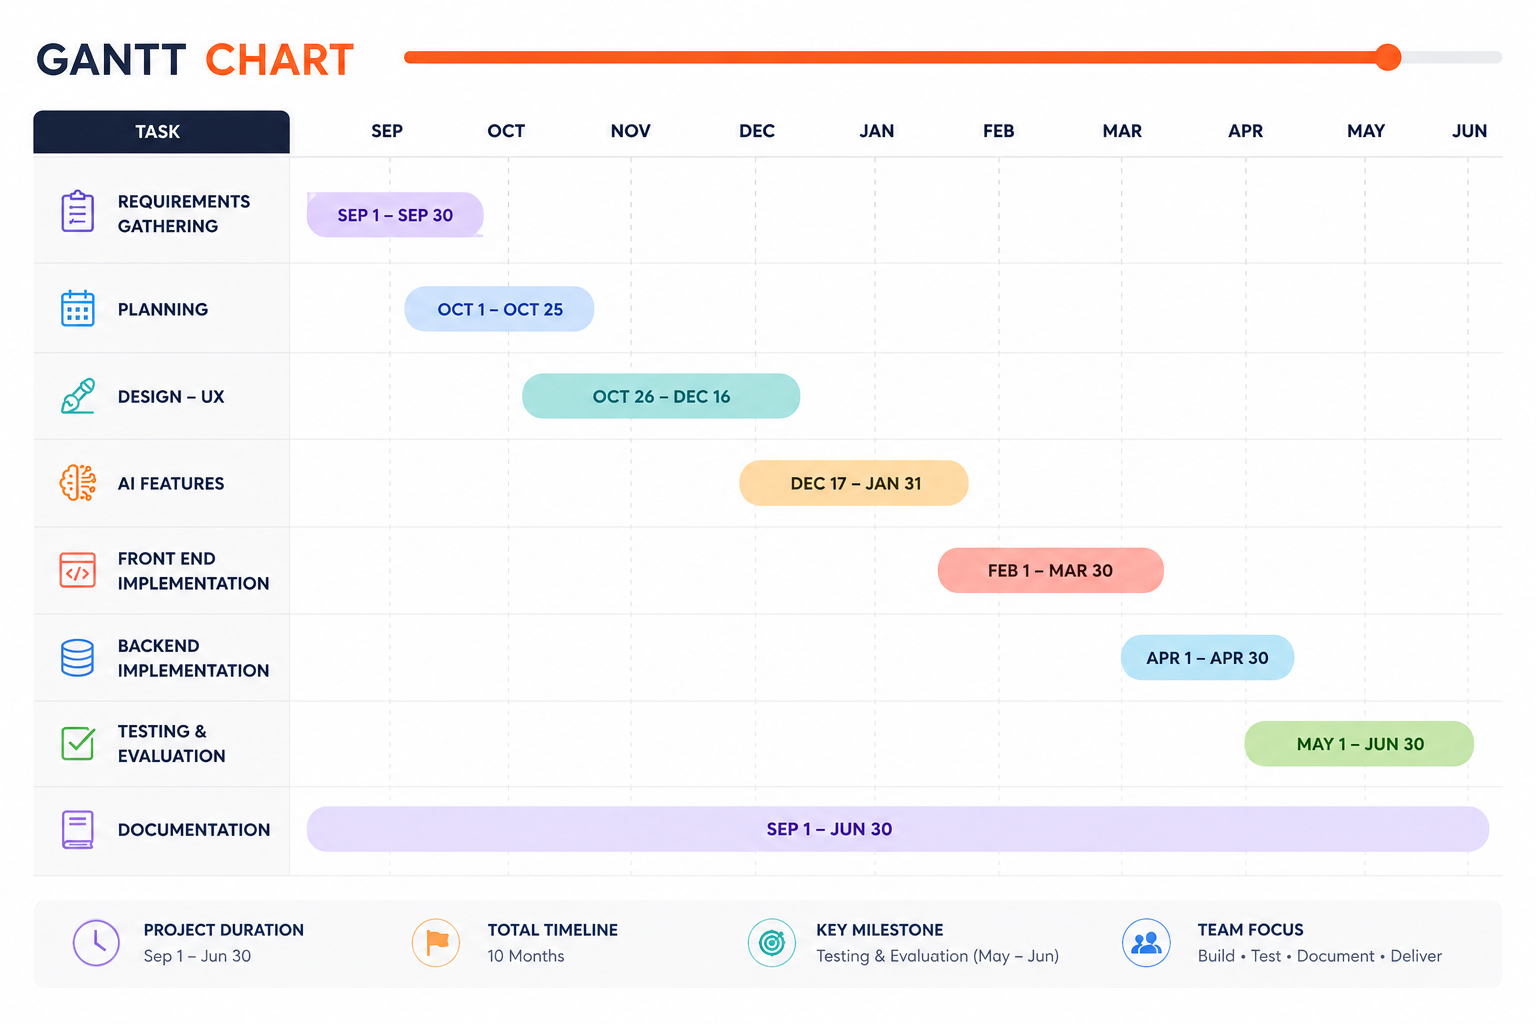
\includegraphics[width=0.95\linewidth,height=0.72\textheight,keepaspectratio]{images/img_033.png}
\caption{Gantt Chart of Project Schedule}
\end{figure}

\section{Functional Requirements}

\textbf{User Authentication \& RBAC:}

Secure login supporting distinct roles: \textbf{Admin}, \textbf{HSE Engineer}, \textbf{Site Supervisor}, and \textbf{Data Analyst}.

Admins possess full privileges for system configuration and user management.

\textbf{Camera Management:}

Admins can add/edit RTSP streams via the Dashboard.

System validates stream connectivity immediately upon entry.

Metadata includes: camera\_id, RTSP\_URL, ROI\_polygon, and location\_tag.

\textbf{Edge AI Engine (Internal Component):}

Autonomous execution of unified hazard inference pipelines for PPE detection, fall detection, unsafe proximity detection, and posture-related ergonomic risk analysis.

\textbf{Face Blurring:} Applied automatically to all detected persons prior to snapshot generation.

\textbf{Hazard Severity Classification:} For each detected hazard (PPE, fall, proximity, posture), the engine assigns an appropriate severity level (e.g., high, medium, low) based on confidence, duration, and hazard type. These severity levels are used by the alerting logic to differentiate between emergency incidents and low-severity ergonomic records.

\textbf{Real-Time Alerting:}

\textbf{Local (Emergency Incidents):} Immediate activation of on-site sirens/lights (latency <1s) \textbf{only} for acute, high-severity safety hazards, namely:

Confirmed fall events.

PPE violations (e.g., missing helmet or vest) above configured thresholds.

Unsafe proximity between workers and hazardous zones or moving equipment.

\textbf{Remote (Emergency Incidents):} Push notifications (FCM) to Supervisors and WebSocket updates to the HQ Dashboard are generated for the same set of acute, high-severity hazard types (falls, PPE violations, unsafe proximity).

\textbf{Non-Emergency Ergonomic Alerts:} Posture-related ergonomic hazards, typically classified as low or medium severity, are logged as \textbf{low-severity ergonomic events} and surfaced in dashboards and reports. They \textbf{do not} trigger sirens or high-priority mobile alerts, thereby avoiding alert fatigue while still providing actionable insights for preventive ergonomics.

\textbf{Event Management \& Lifecycle:}

Structured logging of incidents with timestamp, confidence score, computed severity, and snapshot.

\textbf{Closed-Loop Workflow:} Supervisors must "Acknowledge" alerts and record "Action Taken" to resolve an incident.

\textbf{Health Monitoring:}

Continuous tracking of camera status (Online/Offline), FPS, and connectivity.

Automated reconnection logic with exponential backoff.

\textbf{Privacy \& Retention:}

Strict policy: \textbf{No raw video storage}.

Configurable retention periods for snapshots and metadata, including both incident and ergonomic posture records.

\textbf{Posture \& Ergonomic Risk Assessment:}

The system shall continuously estimate worker body posture using skeletal keypoints extracted from video frames (e.g., shoulders, hips, knees, trunk orientation).

An internal ergonomic scoring mechanism (inspired by standard frameworks such as \textbf{RULA/REBA}) shall classify posture snapshots into low, medium, or high musculoskeletal risk levels.

Non-emergency \textbf{ergonomic alerts} shall be generated for prolonged high-risk postures (e.g., sustained trunk flexion beyond a configurable duration). These are logged as \textbf{low-severity events} and do not activate emergency sirens or high-priority mobile alerts.

Aggregated posture risk data (per worker zone or per camera) shall be stored as \textbf{ergonomic records} and made available to HSE Engineers for trend analysis and preventive intervention planning, helping identify high-risk tasks and areas over time without causing alert fatigue.

\section{Non-Functional Requirements}

\textbf{Performance:}

Target Inference Rate: \textbf{15–30 FPS} (hardware dependent).

End-to-End Latency (Detection to Mobile Alert): \textbf{2–3 seconds}.

\textbf{Scalability:} Horizontal scalability achieved by adding Edge nodes; vertical scalability via model optimization (e.g., quantization).

\textbf{Reliability:} The system must recover automatically from network interruptions and camera signal loss, for both real-time incident detection and continuous posture data collection.

\textbf{Security:}

Data in Transit: TLS/SSL encryption for API and WebSocket connections.

Data at Rest: Encrypted storage for snapshots; hashed passwords.

\section{System Actors and Roles}

\begin{table}[H]
\centering
\small
\renewcommand{\arraystretch}{1.2}
\begin{tabular}{|
>{\RaggedRight\arraybackslash}p{0.24\linewidth}|
>{\RaggedRight\arraybackslash}p{0.68\linewidth}|}
\hline
\textbf{Actor} & \textbf{Responsibilities} \\
\hline
System Administrator & System config, user management, camera setup, health monitoring. \\
\hline
HSE Engineer & Dashboard monitoring, incident investigation, compliance auditing, ergonomic trend analysis. \\
\hline
Site Supervisor & Receives mobile alerts, performs on-site intervention, logs corrective actions. \\
\hline
Data Analyst & Reviews long-term trends, generates safety KPIs and reports. \\
\hline
AI Engine & Internal System Actor. Performs unified hazard detection (PPE, falls, proximity, posture), anonymization, severity classification, and triggers events. \\
\hline
\end{tabular}
\caption{\textbf{System actors and roles}}
\end{table}

\section{Use Case Modeling}

\textbf{Use Case Diagram}

The Use Case diagram provides a high-level view of the system's functional scope and the interactions between actors and use cases. It clearly distinguishes between human actors (Admin, HSE, Supervisor) who interact with the UI, and the \textbf{AI Engine}, which is depicted as a system actor responsible for backend automation. A unified hazard detection use case covers all four hazard categories (PPE violations, falls, unsafe proximity, and posture-related ergonomic risks), while the alerting and reporting interfaces distinguish between emergency incident handling and preventive ergonomic analysis.

While the \textbf{AI Engine} executes hazard detection and posture analysis in a unified pipeline on the Edge node, only acute, high-severity hazards (falls, PPE violations, unsafe proximity) enter the emergency alerting workflow; posture-related deviations, typically of lower severity, are captured as ergonomic records and exposed through analytic views rather than immediate alarms.

\begin{figure}[H]
\centering
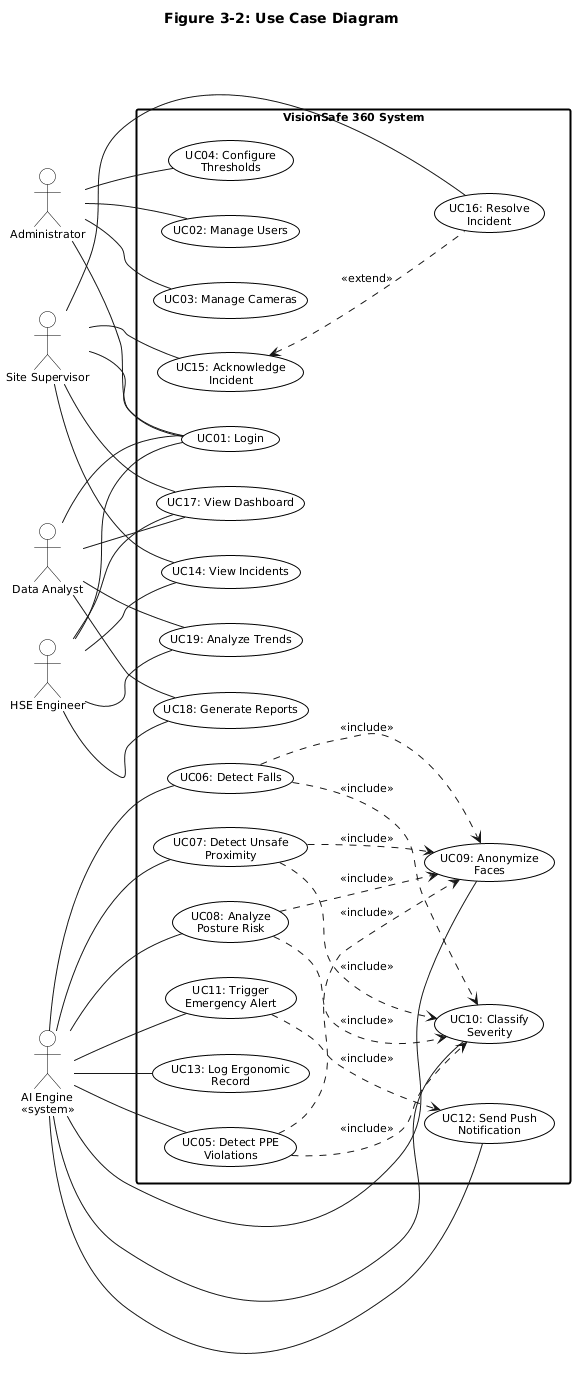
\includegraphics[width=0.95\linewidth,height=0.72\textheight,keepaspectratio]{images/img_007.png}
\caption{Key Use Case Scenarios}
\end{figure}

\textbf{Hazard Detection:} The Edge AI detects a "Fall". The system validates confidence, classifies severity, checks the cooldown timer, triggers the local siren, blurs faces in the frame, and uploads the event to the Backend as an emergency incident.

\textbf{Incident Resolution:} A Supervisor receives a notification, opens the app to view the snapshot, attends to the worker, and marks the incident as "Resolved" with notes.

\textbf{Camera Onboarding:} The Admin inputs an RTSP URL. The system attempts a connection handshake; if successful, the camera is added to the active monitoring pool.

\textbf{Posture Trend Analysis:} The AI Engine periodically evaluates worker posture using skeletal keypoints and assigns ergonomic risk scores (e.g., low/medium/high). These low-severity posture records are aggregated by camera or work zone and later reviewed by HSE Engineers through the dashboard to identify tasks or areas associated with sustained high ergonomic risk.

\section{Activity Diagram}

This diagram details the sequential logic flow of the core detection loop, specifically focusing on how the system handles continuous video frames. It illustrates the critical decision-making process: acquiring a frame, running unified hazard inference (PPE, falls, proximity, posture), validating the detections against confidence thresholds, and then classifying the \textbf{severity} of each hazard. This mechanism is vital to prevent "alert fatigue" by ensuring that only genuinely high-severity, acute hazards (e.g., a confirmed fall with high confidence) can trigger immediate emergency alerts.

In parallel, or rather as part of the unified hazard analysis, posture-related ergonomic hazards are evaluated and assigned typically low or medium severity levels. These posture hazards generate \textbf{non-emergency, low-severity posture records} for long-term musculoskeletal risk assessment. These posture-related records do not trigger real-time sirens or high-priority alerts but instead feed ergonomic dashboards and reports for HSE teams.

\begin{figure}[H]
\centering
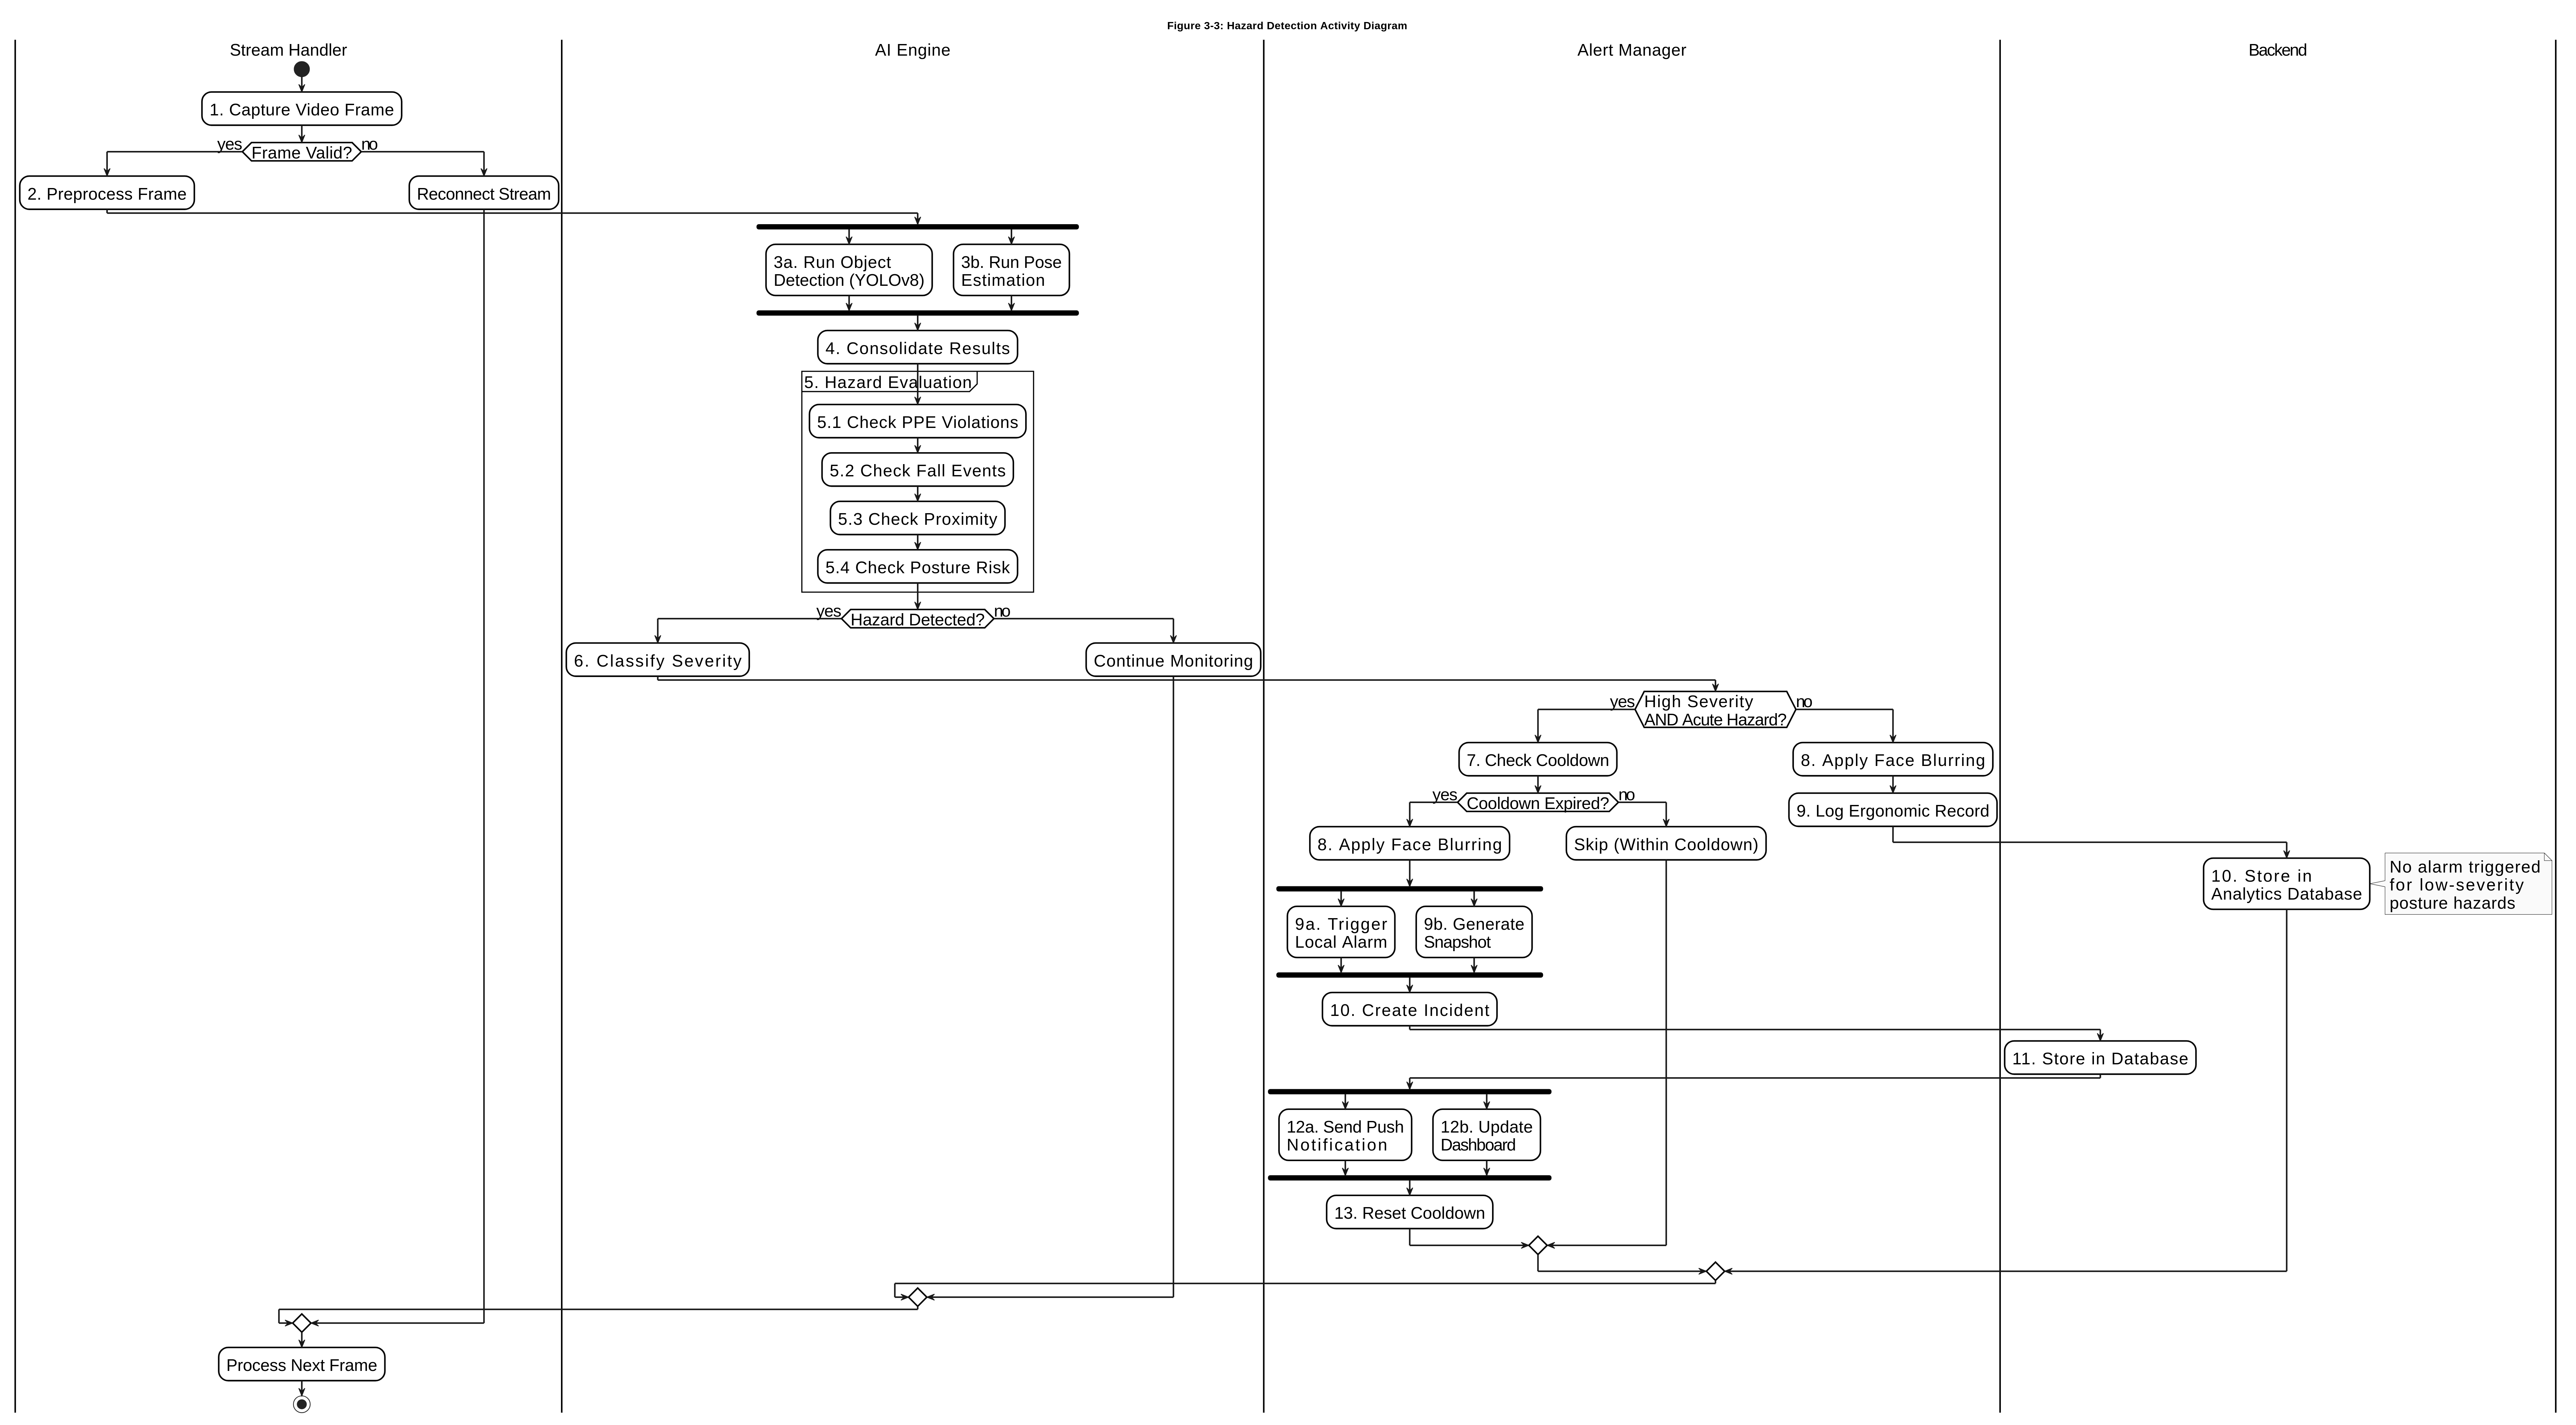
\includegraphics[width=0.95\linewidth,height=0.72\textheight,keepaspectratio]{images/img_008.png}
\caption{Activity Diagram}
\end{figure}

\textbf{Flow Summary:}

Capture Frame → Unified Inference (PPE/Fall/Proximity/Posture) → Hazard Evaluation → Severity Classification →

\textbf{If High/Critical \& Acute Hazard (PPE/Fall/Proximity):}

Cooldown Check → Trigger Alarm → Anonymize \& Save → Notify Backend (Incidents)

\textbf{Else (Low/Medium Severity, including most Posture cases):}

Log Ergonomic / Low-Severity Record → Notify Backend (Analytics/Ergonomics).

\section{Data Flow Diagram (DFD)}

\textbf{Level 0 (Context Diagram)}

The Context Diagram (Level 0) defines the system boundary of VisionSafe 360. It illustrates the external entities that interact with the system: \textbf{Cameras} (Input source), \textbf{Site Supervisors/HSE} (Notification recipients and ergonomic data consumers), and \textbf{Admins} (Configuration). The central process represents the entire VisionSafe system, abstracting internal complexities to focus on input/output data streams, including both real-time emergency incident alerts and longer-term ergonomic posture records.

\begin{figure}[H]
\centering
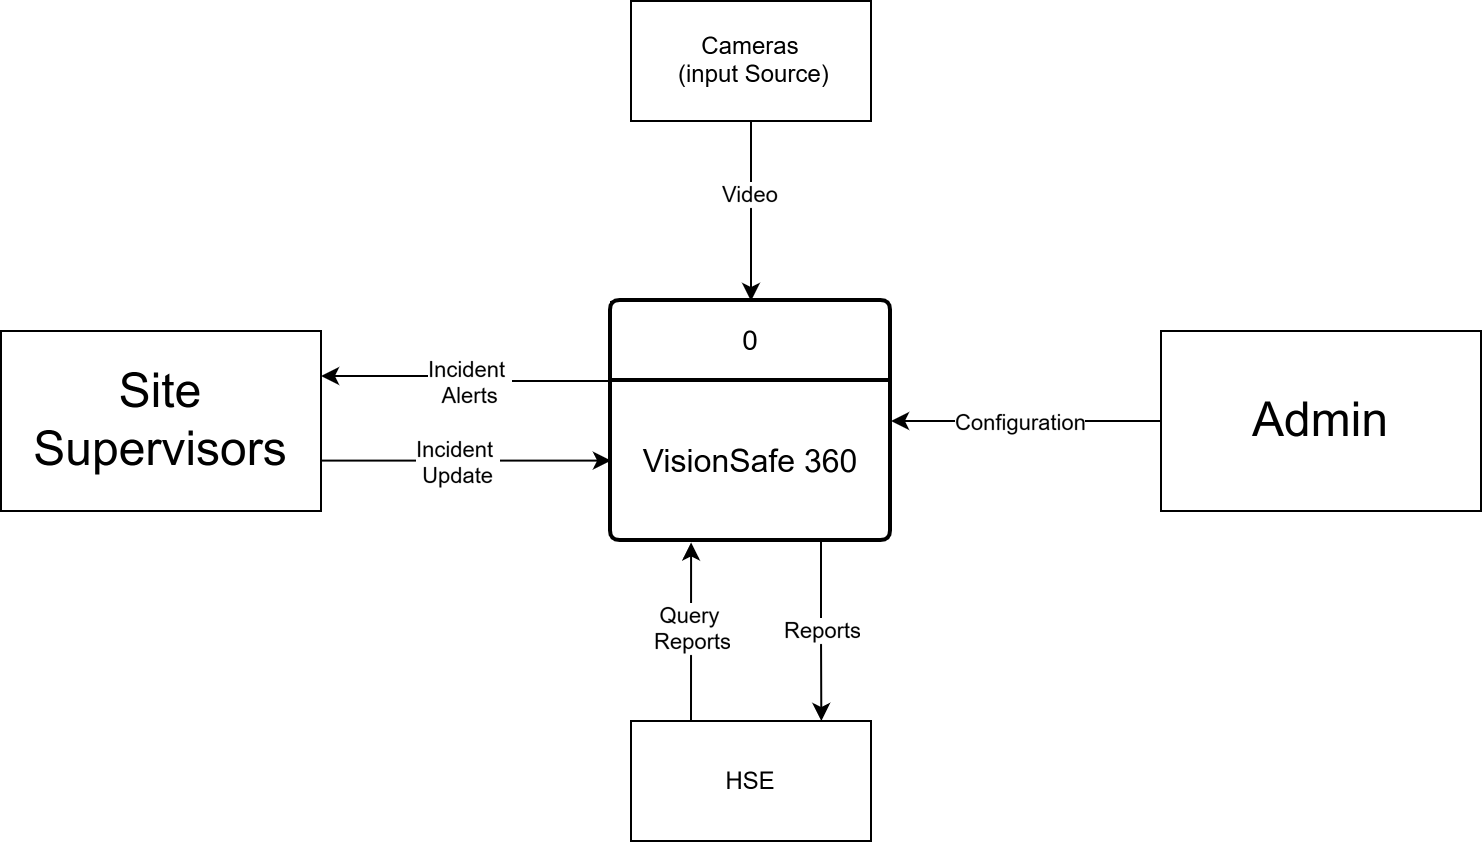
\includegraphics[width=0.95\linewidth,height=0.72\textheight,keepaspectratio]{images/img_009.png}
\caption{Context Diagram}
\end{figure}

\textbf{Level 1 Diagram}

The Level 1 DFD decomposes the system into its primary subsystems to show detailed data routing:

\textbf{Ingestion \& Processing:} RTSP streams enter the Edge module where unified hazard inference (PPE, falls, proximity, posture) and face blurring occur. Hazard evaluation and severity classification are applied to all hazard categories.

\textbf{Transmission:} Only metadata and encrypted snapshots are passed to the \textbf{API Gateway}. This includes both hazard metadata for acute, high-severity incidents (e.g., falls, PPE violations, unsafe proximity) and posture-related ergonomic scores and durations (typically logged as low-severity records for trend analysis).

\textbf{Storage:} Structured data is persisted in the SQL Database, with separate fields or records representing emergency incidents (e.g., falls, PPE violations) and non-emergency ergonomic observations (e.g., high-risk posture episodes).

\textbf{Presentation:} The Backend serves data to the Web Dashboard and pushes notifications to Mobile Clients. HSE Engineers can review both real-time emergency alerts (for acute hazards) and aggregated low-severity ergonomic posture trends to inform preventive interventions without overwhelming supervisors with immediate alarms.

\begin{figure}[H]
\centering
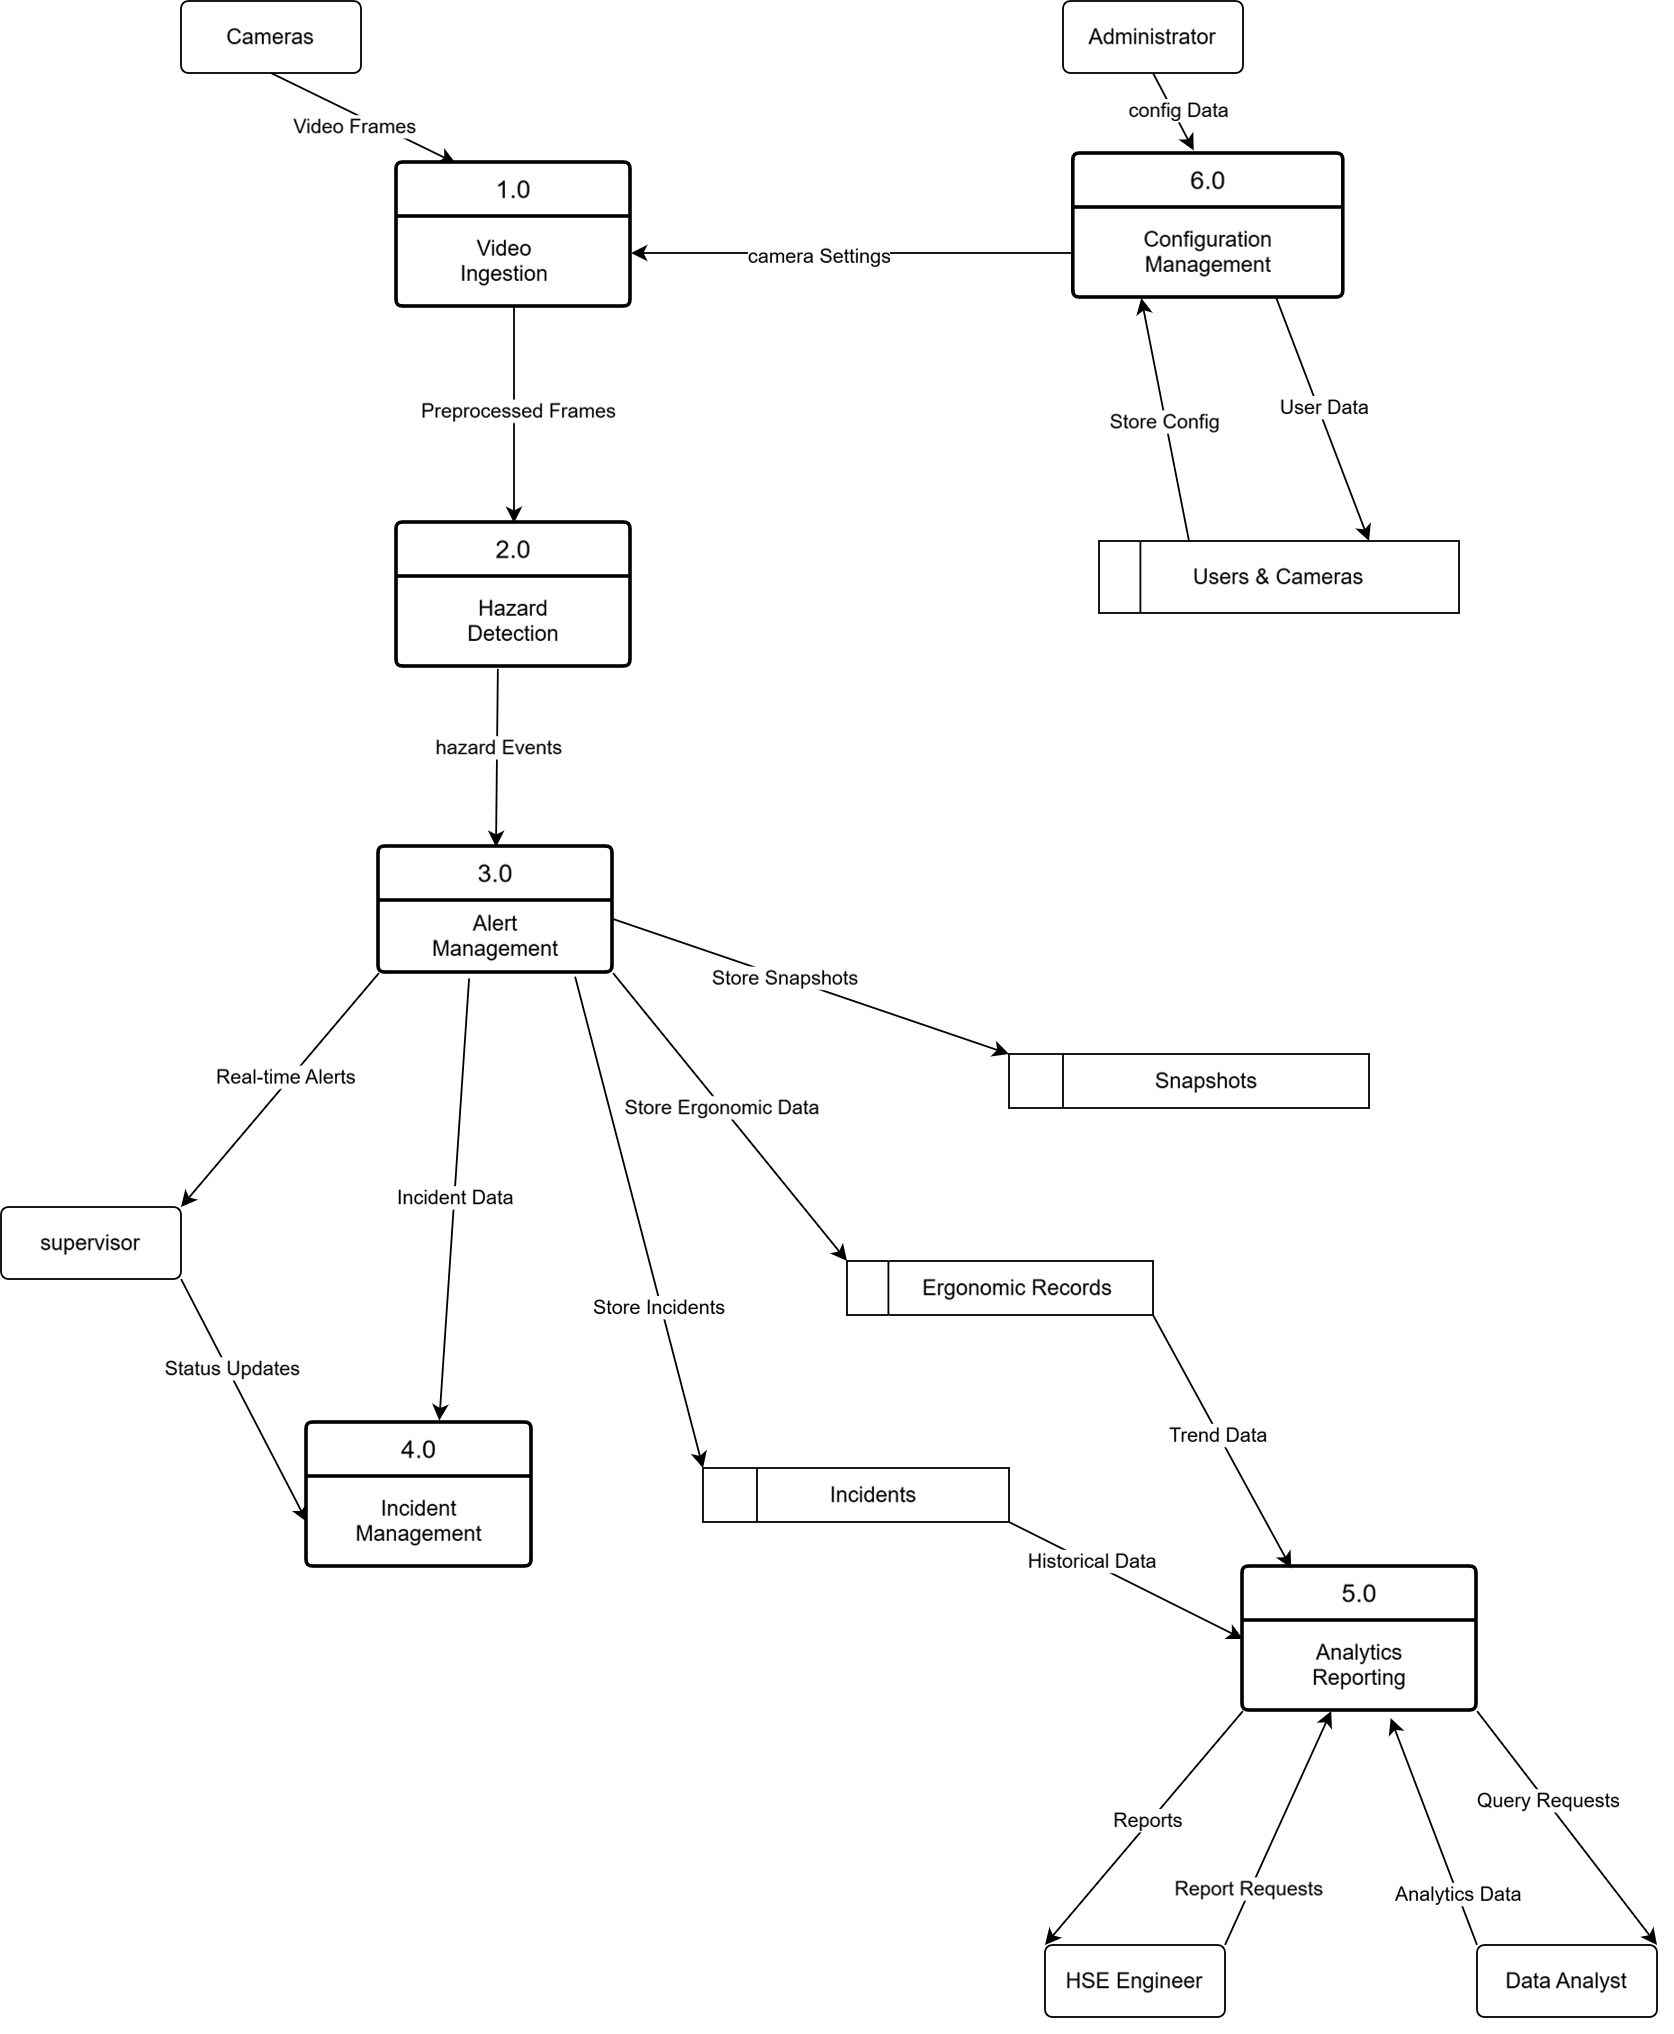
\includegraphics[width=0.95\linewidth,height=0.72\textheight,keepaspectratio]{images/img_010.png}
\caption{Data Flow Diagram (Level 1)}
\end{figure}

\section{Entity Relationship Diagram (ERD)}

The ERD visualizes the database schema designed to support the system's data persistence requirements. It employs a normalized relational structure to ensure data integrity. The central entity is the \textbf{Incident}, which links \textbf{Cameras} (where it happened), \textbf{Hazard Types} (what happened), and \textbf{Users} (who resolved it). This structure supports complex queries for analytics, such as "Total PPE violations per camera per week". Posture-related ergonomic risks are represented as hazard types of lower severity (e.g., POSTURE\_RISK) and can be queried independently or alongside other hazards to understand both acute and chronic risk patterns.

\begin{figure}[H]
\centering
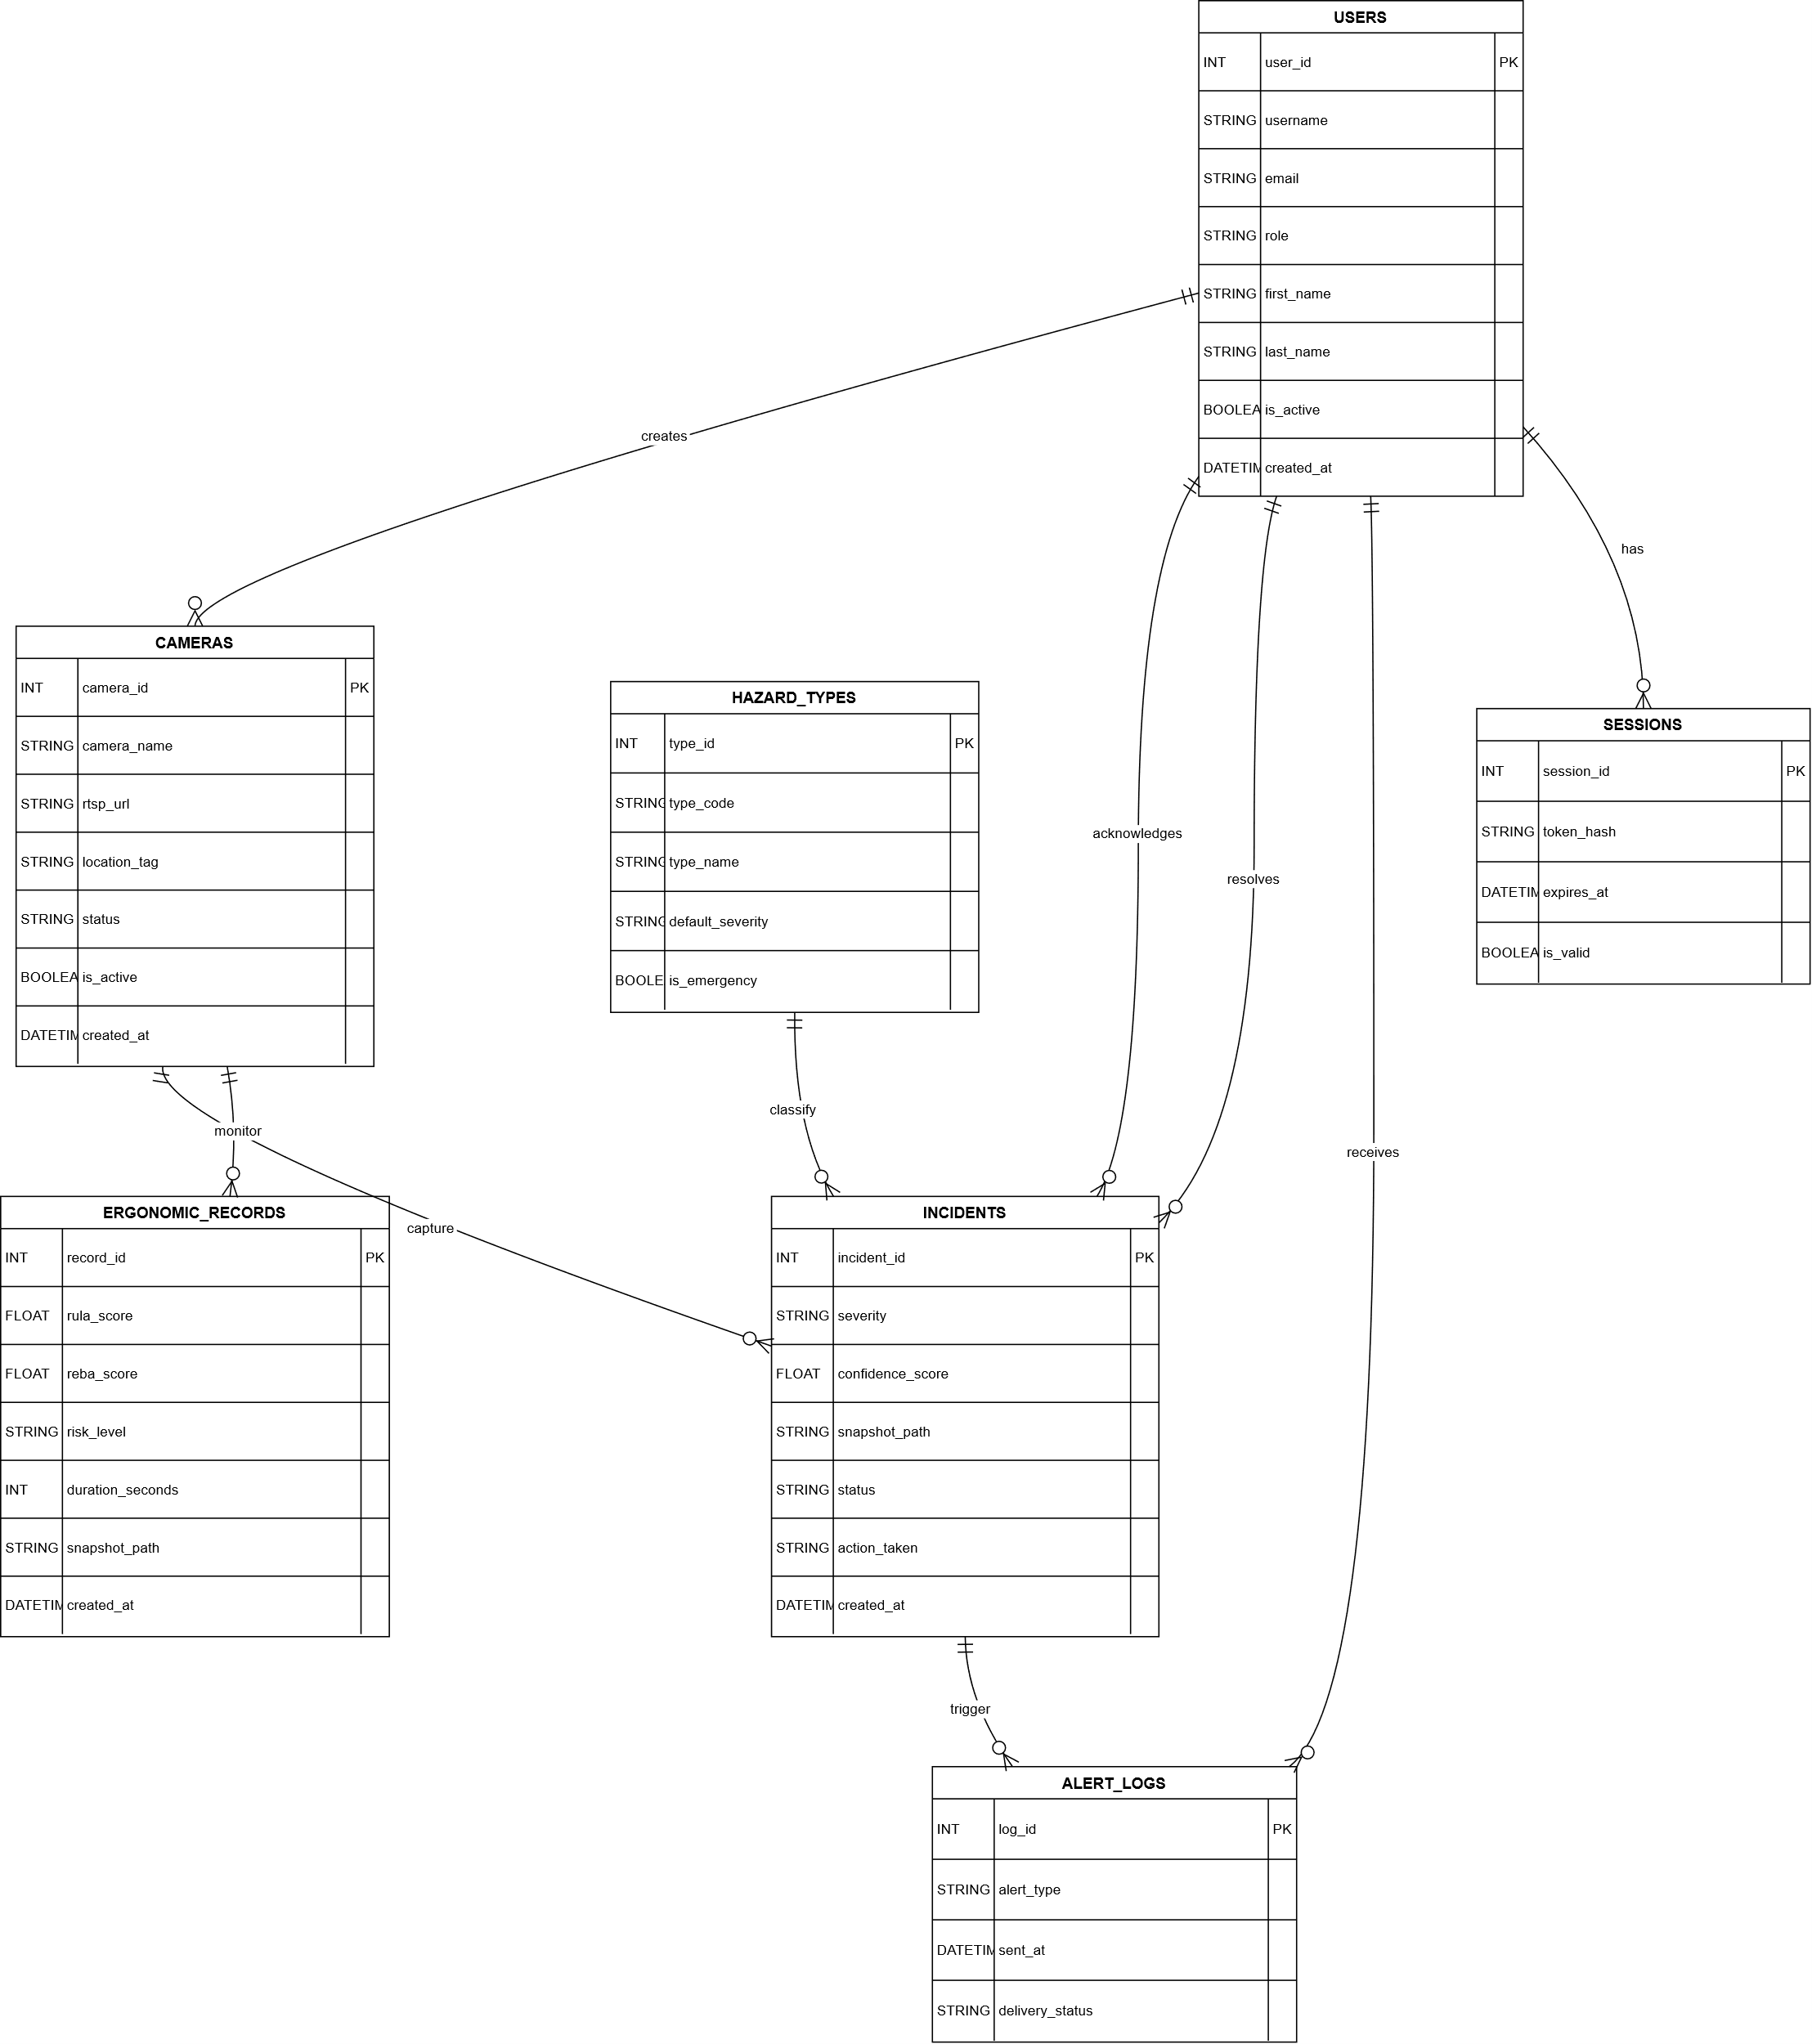
\includegraphics[width=0.95\linewidth,height=0.72\textheight,keepaspectratio]{images/img_011.png}
\caption{Entity Relationship Diagram}
\end{figure}

\textbf{Key Entities:}

\textbf{Users:} Stores authentication credentials, roles, and FCM tokens for mobile pushes.

\textbf{Cameras:} Contains configuration data including RTSP URLs and JSON-defined Region of Interest (ROI) polygons.

\textbf{Incidents:} The core transactional table storing event timestamps, confidence scores, severity, snapshot paths, and resolution status. This includes safety-critical events (e.g., falls) and may also reference posture-related events classified as low-severity when needed for ergonomic analysis.

\textbf{HazardTypes:} A lookup table defining detectable classes (e.g., "No Helmet", "Fall", "Proximity", "Posture Risk") and their associated default severitylevels.

\section{Class Diagram}

The Class Diagram represents the static structure of the software implementation, adhering to Object-Oriented Design (OOD) principles. It highlights the modular separation of concerns:

\textbf{StreamHandler:} Responsible solely for video I/O, frame buffering, and connection health.

\textbf{InferenceEngine:} Wraps the YOLO model (and any auxiliary pose estimation models), handling pre-processing and post-processing of tensors.

\textbf{HazardAnalyzer:} Contains the business logic for unified hazard evaluation (PPE, falls, proximity, posture). It generates hazard events enriched with type and severity information.

\textbf{PostureAnalyzer:} A dedicated analytic component that consumes frames and/or pose data to extract skeletal keypoints, compute ergonomic scores (e.g., RULA/REBA-inspired), and provide posture-related hazard candidates and risk levels to the HazardAnalyzer.

\textbf{Alerting/Notification Logic (e.g., AlertManager + NotificationService):} Applies an alert routing policy based on hazard severity and type:

High/Critical severity for acute hazards (falls, PPE, proximity) → emergency sirens and incident creation.

Low/Medium severity, especially posture-related ergonomic hazards → ergonomic records and analytic logging only (no sirens).

\textbf{NotificationService:} An interface for triggering external actions (Sirens, API calls) without coupling the core logic to specific output hardware.

The PostureAnalyzer and HazardAnalyzer jointly implement a unified hazard detection pipeline, while the alerting logic enforces different behaviors for emergency incidents versus low-severity ergonomic records.

\begin{figure}[H]
\centering
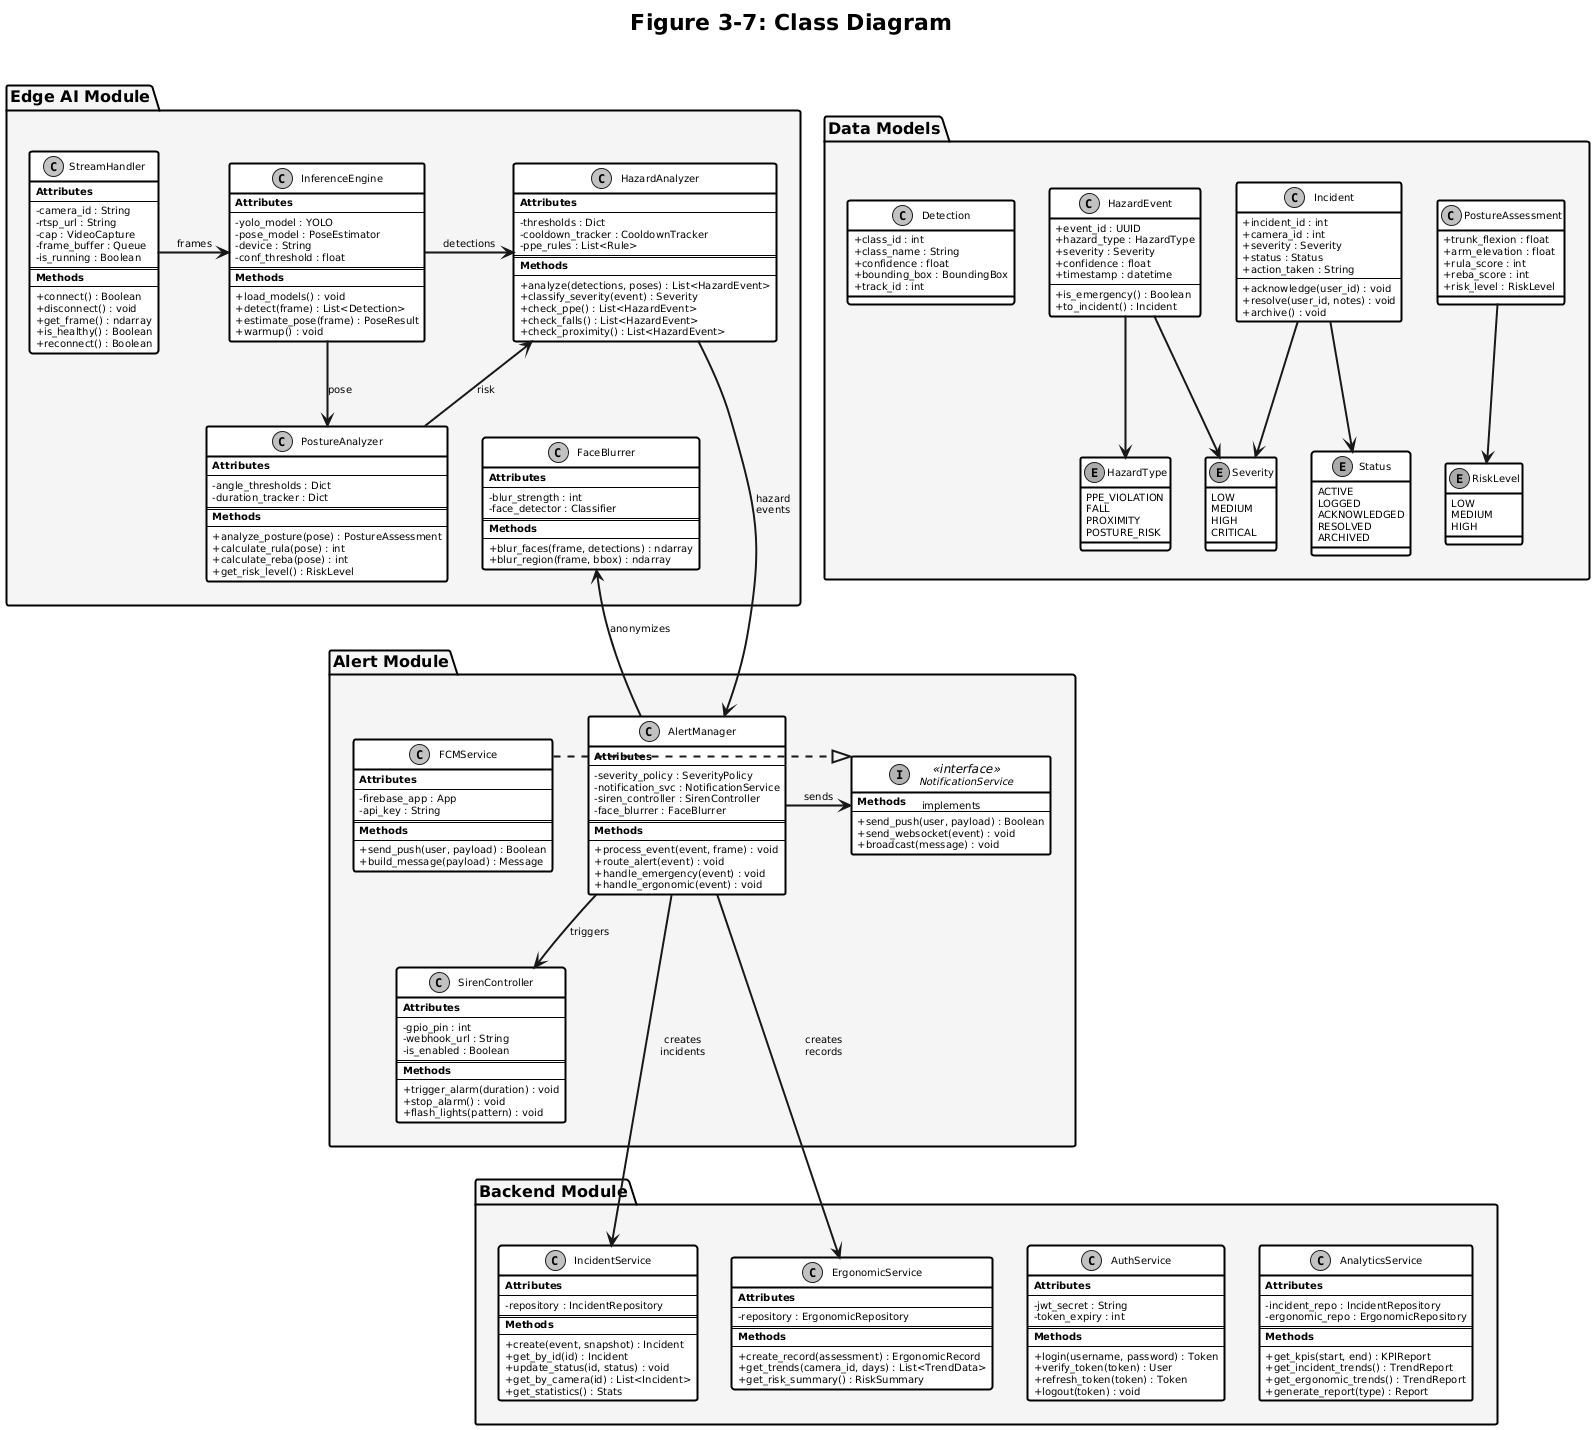
\includegraphics[width=0.95\linewidth,height=0.72\textheight,keepaspectratio]{images/img_012.png}
\caption{Class Diagram}
\end{figure}

\section{Sequence Diagram}

The Sequence Diagram provides a dynamic view of the system, capturing the chronological order of interactions during a "Hazard Detection" scenario. It traces the lifecycle of a single video frame: from capture by the \textbf{StreamHandler}, through unified hazard analysis by the \textbf{InferenceEngine}, \textbf{PostureAnalyzer}, and \textbf{HazardAnalyzer}, to the final alerts triggered (or not triggered) by the alerting logic and received by the \textbf{Mobile Client}.

In this workflow, a unified hazard event is created, containing both the hazard type (PPE, fall, proximity, posture) and its severity (e.g., high/medium/low). The alerting logic then decides whether this event becomes an emergency incident (with sirens and mobile alerts) or a low-severity ergonomic record suitable for trend analysis. This diagram is critical for understanding the latency and dependencies between the Edge and Backend components, as well as the separation between emergency incident handling (high-severity PPE/fall/proximity) and continuous, preventive ergonomic analysis (typically low-severity posture hazards) that avoids contributing to alert fatigue.

\begin{figure}[H]
\centering
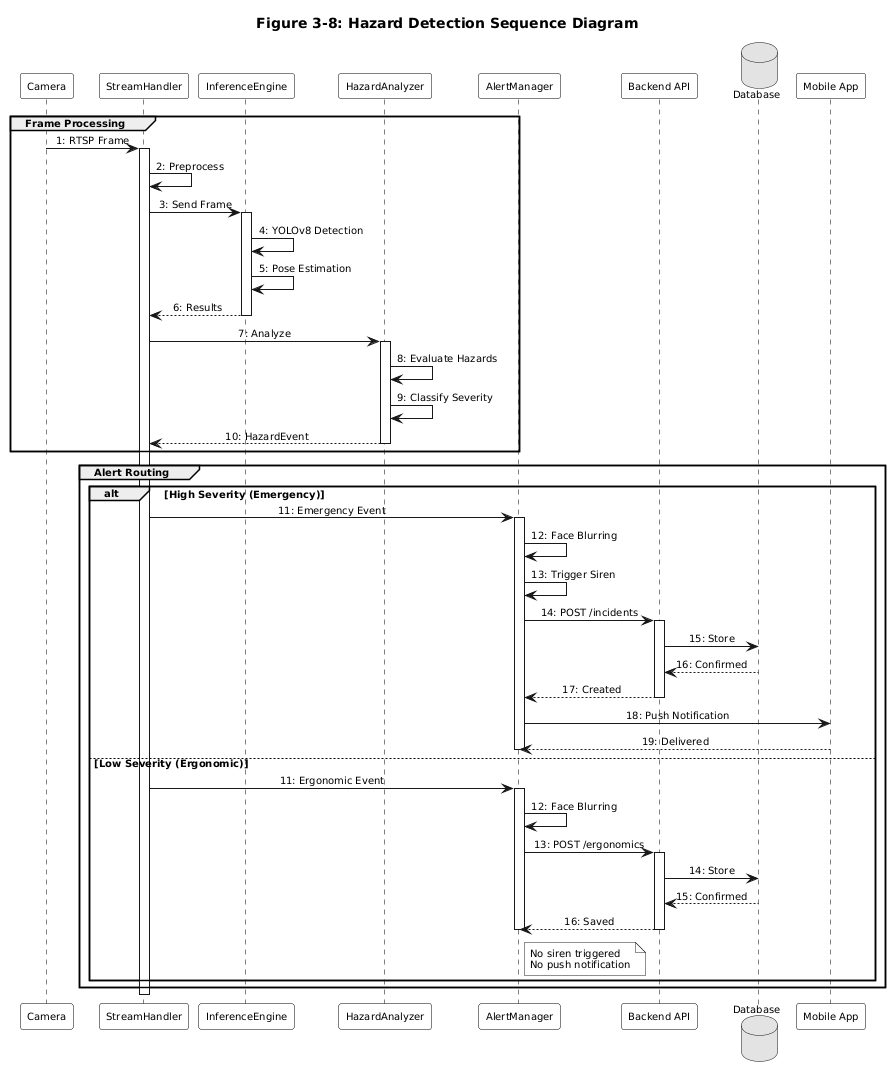
\includegraphics[width=0.95\linewidth,height=0.72\textheight,keepaspectratio]{images/img_013.png}
\caption{Sequence Diagram}
\end{figure}

\textbf{Sequence Steps:}

\textbf{StreamHandler} provides a frame to \textbf{InferenceEngine}.

\textbf{InferenceEngine} returns detection bounding boxes and pose-related keypoints to \textbf{HazardAnalyzer} and \textbf{PostureAnalyzer}.

\textbf{PostureAnalyzer} evaluates skeletal keypoints, computes ergonomic scores, and provides posture-related hazard candidates to \textbf{HazardAnalyzer}.

\textbf{HazardAnalyzer} consolidates PPE, fall, proximity, and posture-related inputs, confirms validity (rules + thresholds), and produces hazard events enriched with \textbf{hazard type and severity}.

The alerting logic (e.g., AlertManager + NotificationService) inspects each hazard event:

For high-severity acute hazards (e.g., falls, PPE, proximity), it triggers local hardware (sirens/lights) and posts an incident to the \textbf{Backend API}.

For low-severity posture-related ergonomic hazards, it bypasses sirens and posts an ergonomic record to the \textbf{Backend API} asynchronously.

\textbf{Backend} persists both emergency incidents and ergonomic records and pushes a real-time update to the \textbf{Mobile Client} (for incidents) and posture dashboards (for HSE Engineers).

\section{Incident Lifecycle \& State Transition}

This State Transition Diagram models the lifecycle of an Incident object, ensuring accountability and workflow enforcement. It defines how an incident moves from being a raw detection to a closed case. This prevents incidents from being "lost" and mandates human intervention for closure.

\begin{figure}[H]
\centering
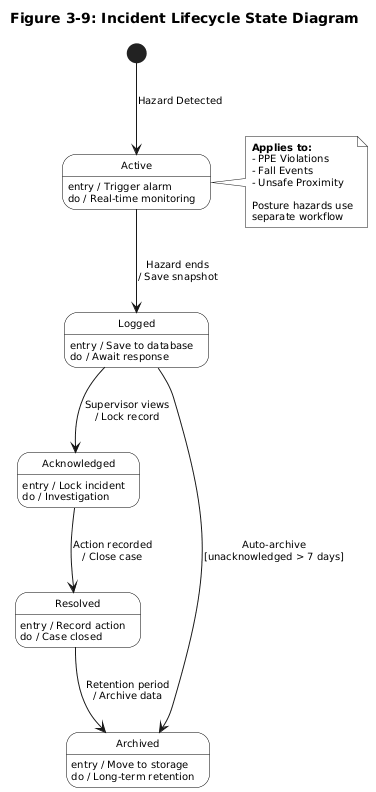
\includegraphics[width=0.95\linewidth,height=0.72\textheight,keepaspectratio]{images/img_014.png}
\caption{State Diagram}
\end{figure}

\textbf{Active:} The hazard is currently detected; alerts are firing.

\textbf{Logged:} The hazard has ceased or stabilized; the event is saved in the DB but requires attention.

\textbf{Acknowledged:} A Supervisor has viewed the notification (locking the incident).

\textbf{Resolved:} Corrective action has been logged, and the case is closed.

\textbf{Archived:} Old data is moved to cold storage for long-term retention.

The Incident lifecycle focuses on acute, high-severity, safety-critical events (such as PPE violations, falls, and unsafe proximity). Posture-related ergonomic observations, typically classified as low or medium severity, are treated as \textbf{non-critical records} and do not enter the emergency incident lifecycle. Instead, they are stored as ergonomic events associated with cameras or work zones, supporting long-term analysis and preventive ergonomics rather than immediate alarm escalation.

\section{Component Diagram}

The Component Diagram illustrates the high-level modular decomposition of VisionSafe 360 and clarifies the responsibilities and interfaces between subsystems across the Edge and Backend environments. It emphasizes the system’s design principle of keeping safety-critical inference and privacy enforcement on-premise (Edge), while delegating persistence, analytics, and multi-client distribution to the Backend.

At the Edge Node, the Stream Handler ingests RTSP camera streams and provides frames to the AI Engine for unified hazard inference. The Posture Analyzer operates alongside the core inference pipeline to estimate skeletal keypoints and compute ergonomic risk indicators, which are then consolidated within the hazard evaluation flow. Prior to any persistence or transmission, the Face Blurring component enforces privacy by anonymizing detected persons. An Alert Controller orchestrates event routing, ensuring that high-severity acute hazards trigger local alarms (via GPIO) while posture-related ergonomic risks are typically logged as low-severity records for trend analysis.

On the Backend Server, an API Gateway exposes secured endpoints and routes requests to specialized services, including Authentication, Incident Management, Ergonomic Records, and Analytics. Data persistence is handled through a dedicated Data Layer, where structured records are stored in PostgreSQL, frequently accessed data is optimized using Redis cache, and encrypted snapshots are stored in file storage. External services such as Firebase FCM are integrated to deliver push notifications to client applications, including the Mobile App and Web Dashboard.

\begin{figure}[H]
\centering
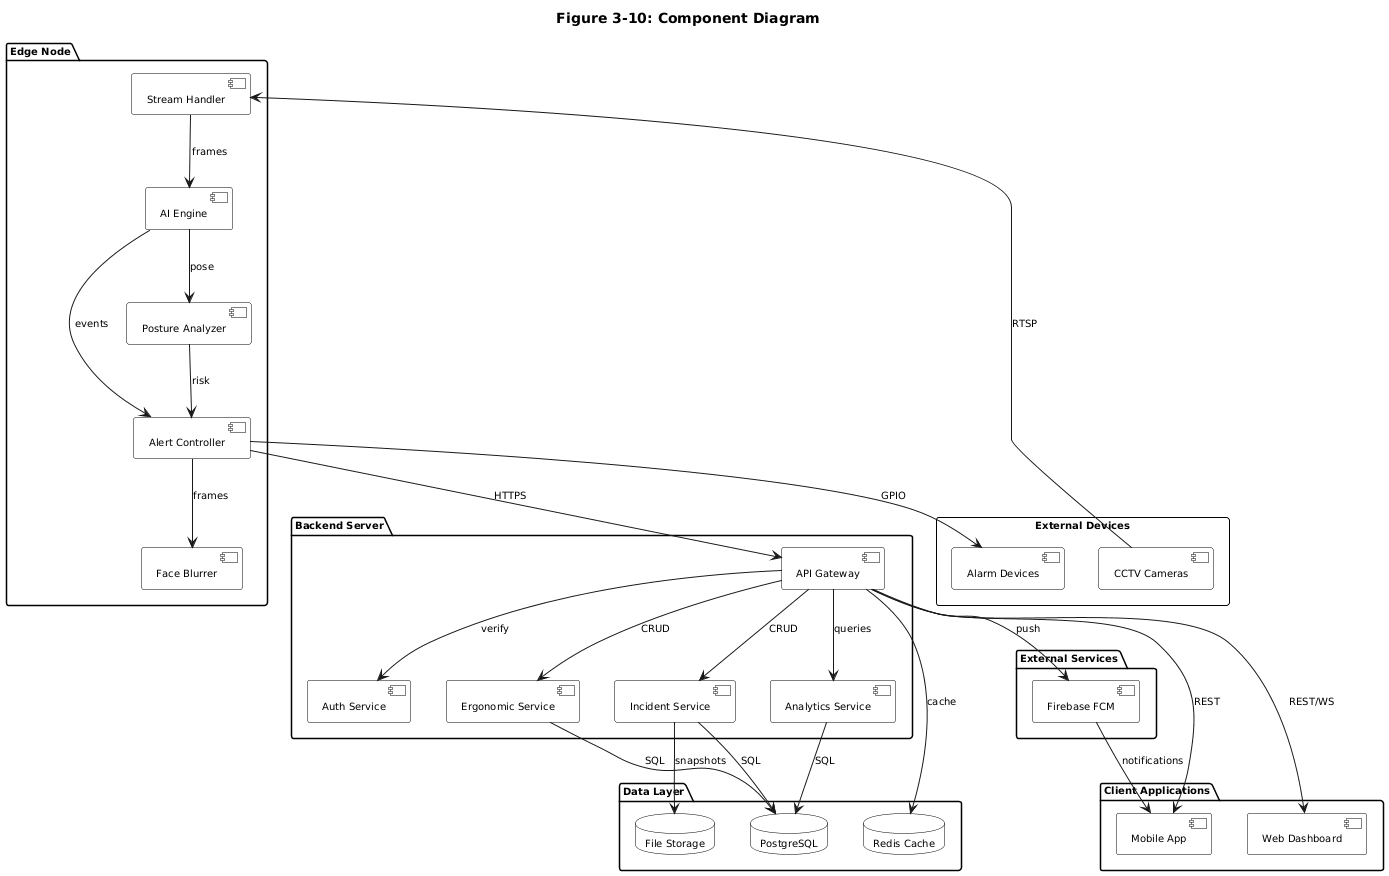
\includegraphics[width=0.95\linewidth,height=0.72\textheight,keepaspectratio]{images/img_015.png}
\caption{Component Diagram}
\end{figure}

\section{Deployment Diagram}

The Deployment Diagram presents the physical runtime topology of VisionSafe 360 across an industrial site and cloud infrastructure. It highlights how the system integrates with existing CCTV installations while ensuring low latency for emergency response and preserving privacy by keeping raw video on-site.

Within the Industrial Site, multiple IP cameras stream video over RTSP to the Edge Server (e.g., NVIDIA Jetson). The Edge node hosts the core runtime modules—stream handling, inference execution, and alert management—along with the primary AI models (YOLOv8 for detection and a lightweight pose model for posture estimation). For immediate on-site response, the Edge Server interfaces with the Alarm System (e.g., siren and strobe light) through GPIO, enabling sub-second activation for confirmed high-severity hazards.

The Cloud Infrastructure hosts the application layer responsible for orchestration and user-facing services, including the FastAPI Backend and a WebSocket server for real-time dashboard updates. Persistent storage is provided through PostgreSQL for structured incident/ergonomic records, Redis for caching and performance optimization, and dedicated file storage for encrypted snapshots. Firebase FCM is used as an external notification layer for mobile push delivery. Client devices (desktop web browser and iOS/Android mobile app) communicate with the backend using secure channels (HTTPS/WSS), receiving emergency incident notifications and accessing analytics views, including aggregated ergonomic posture risk trends.

This deployment layout supports scalability (by adding Edge nodes per site/camera cluster), ensures operational resilience under limited connectivity, and enforces privacy compliance by restricting raw video processing and anonymization to the on-premise Edge environment.

\begin{figure}[H]
\centering
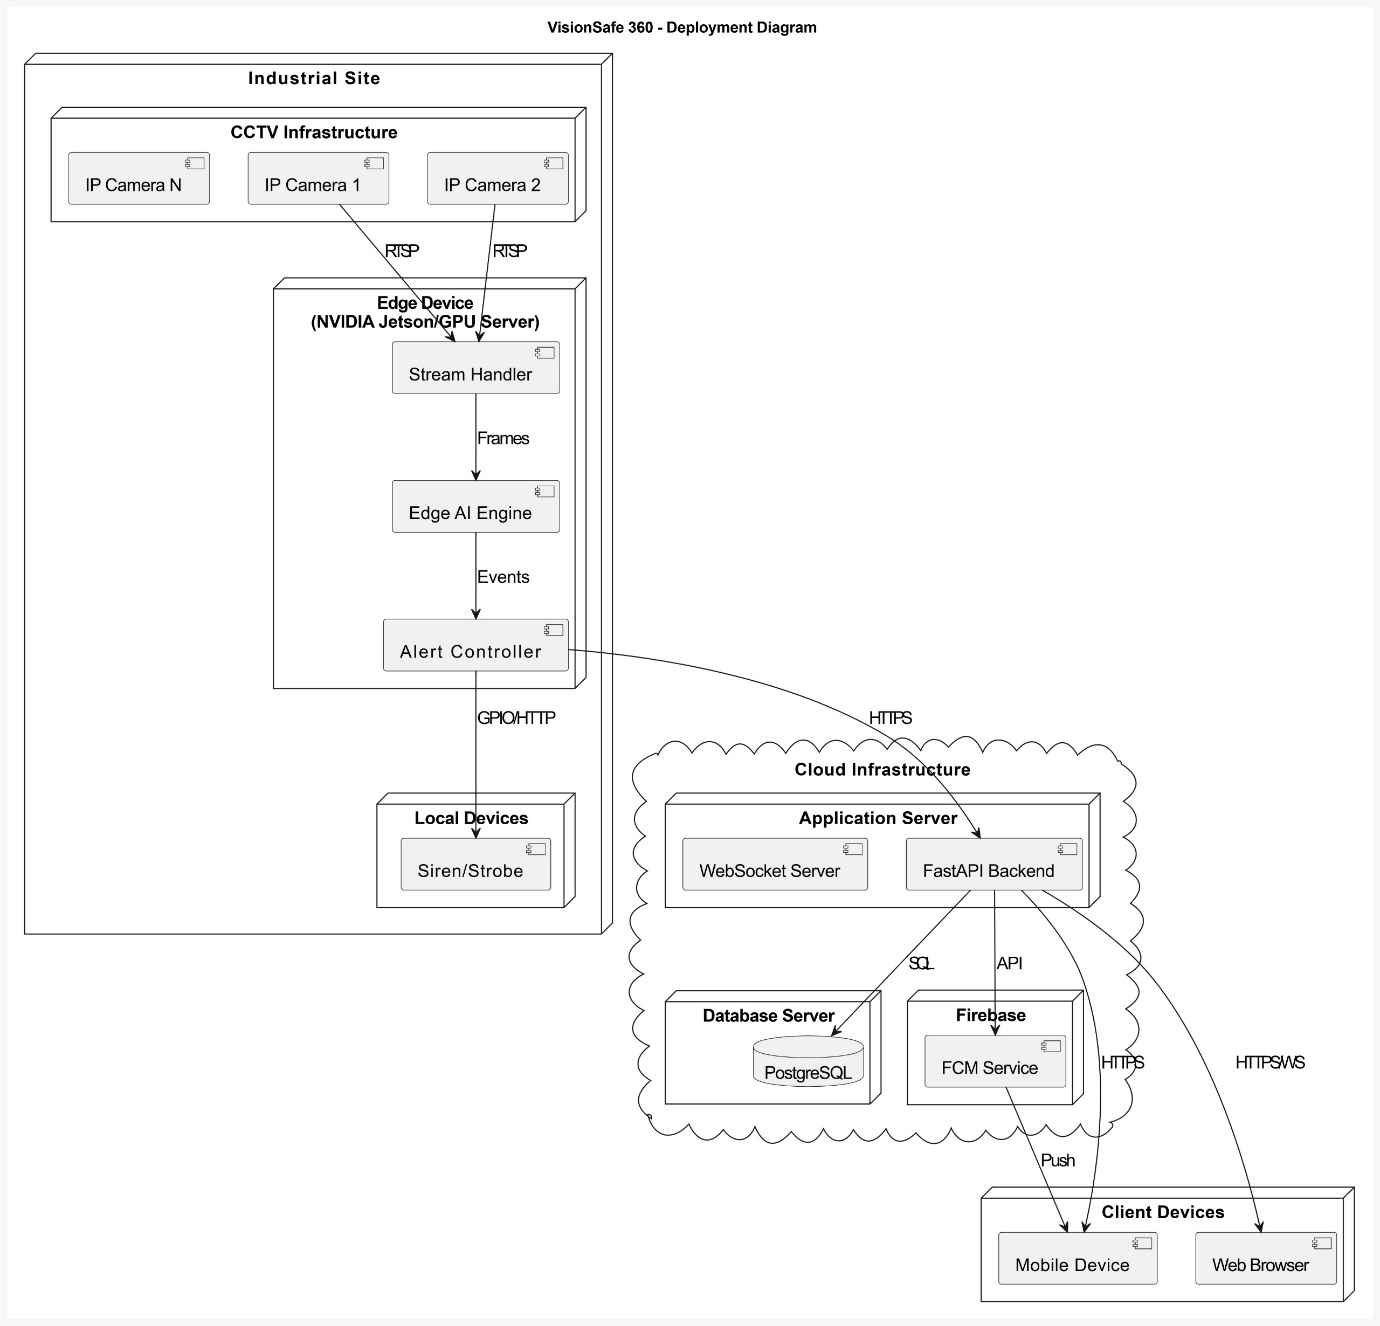
\includegraphics[width=0.95\linewidth,height=0.72\textheight,keepaspectratio]{images/img_016.jpeg}
\caption{Deployment Diagram}
\end{figure}

\section{API Specification Summary}

The communication between the Edge module, Dashboard, and Mobile App is mediated by a RESTful API. The following summary outlines the primary endpoints, all secured via JWT authentication:

POST /auth/login: Authenticates users and returns access tokens.

GET /cameras/health: Returns real-time status (Online/Offline/FPS) of all streams.

POST /incidents: Internal endpoint for the Edge Engine to upload new emergency incidents (generally high-severity PPE, fall, and proximity hazards).

PATCH /incidents/\{id\}: Used by Supervisors to update incident status and add "Action Taken" notes.

WS /events: A WebSocket endpoint providing a live feed of emergency incident events to the dashboard.

(Optionally) POST /ergonomics: Internal endpoint for uploading \textbf{non-emergency, low-severity posture records and ergonomic risk scores} for trend analysis, feeding dashboards and reports rather than immediate emergency alerting.

\section{Chapter Summary}

This chapter provided a comprehensive analysis of VisionSafe 360. It defined the problem scope, analyzed operational constraints, and detailed the functional and non-functional requirements necessary for a robust safety solution. The system architecture-prioritizing \textbf{Edge computing} for latency and privacy—was modeled through standard UML diagrams (Use Case, Activity, Class, Sequence) and Data Flow Diagrams.

The design incorporates a \textbf{unified, AI-driven hazard detection pipeline} covering four hazard categories: \textbf{PPE detection}, \textbf{fall detection}, \textbf{unsafe proximity monitoring}, and \textbf{Posture-related Ergonomic Risk Analysis}. A severity-aware alerting policy clearly distinguishes between emergency incident handling—reserved for high-severity, acute hazards—and continuous, preventive ergonomic risk monitoring for posture-related hazards. Within this architecture, acute hazards (PPE violations, falls, unsafe proximity) drive the real-time emergency alerting workflow, whereas posture-related ergonomic deviations are continuously monitored and recorded as low-severity events for long-term trend analysis and preventive ergonomics, thereby supporting HSE teams without introducing additional alert fatigue. These design specifications lay the groundwork for \textbf{Chapter 4}, which will detail the implementation of the inference pipelines, backend services, and interface integration.

\chapter{Project Design}

\section{Overview of the Design}

VisionSafe 360 is designed as a user-centered safety monitoring ecosystem for industrial and construction environments. The project focuses on converting raw safety observations into actionable intelligence to reduce incident response time and improve long-term preventive safety practices.

The primary objective is to manage four critical workplace risks: PPE compliance, fall events, unsafe proximity, and ergonomic hazards. The design distinguishes between \textbf{Emergency Response} (immediate action) and \textbf{Preventive Analytics} (long-term trends), ensuring that safety-critical events are surfaced with urgency while minimizing alert fatigue for long-term data. The design ensures a seamless integration between high-level oversight and rapid field-level intervention.

\section{System Architecture}

\textbf{Overall Architecture}

The system is structured as a modular, cross-platform architecture designed to support two distinct interaction environments:

\textbf{Control Room Environment (Web Dashboard):} Optimized for continuous situational awareness, detailed incident investigation, and administrative oversight.

\textbf{On-Site Response Environment (Mobile App):} Tailored for rapid alert reception, immediate acknowledgement, and field-level resolution logging.

\begin{figure}[H]
\centering
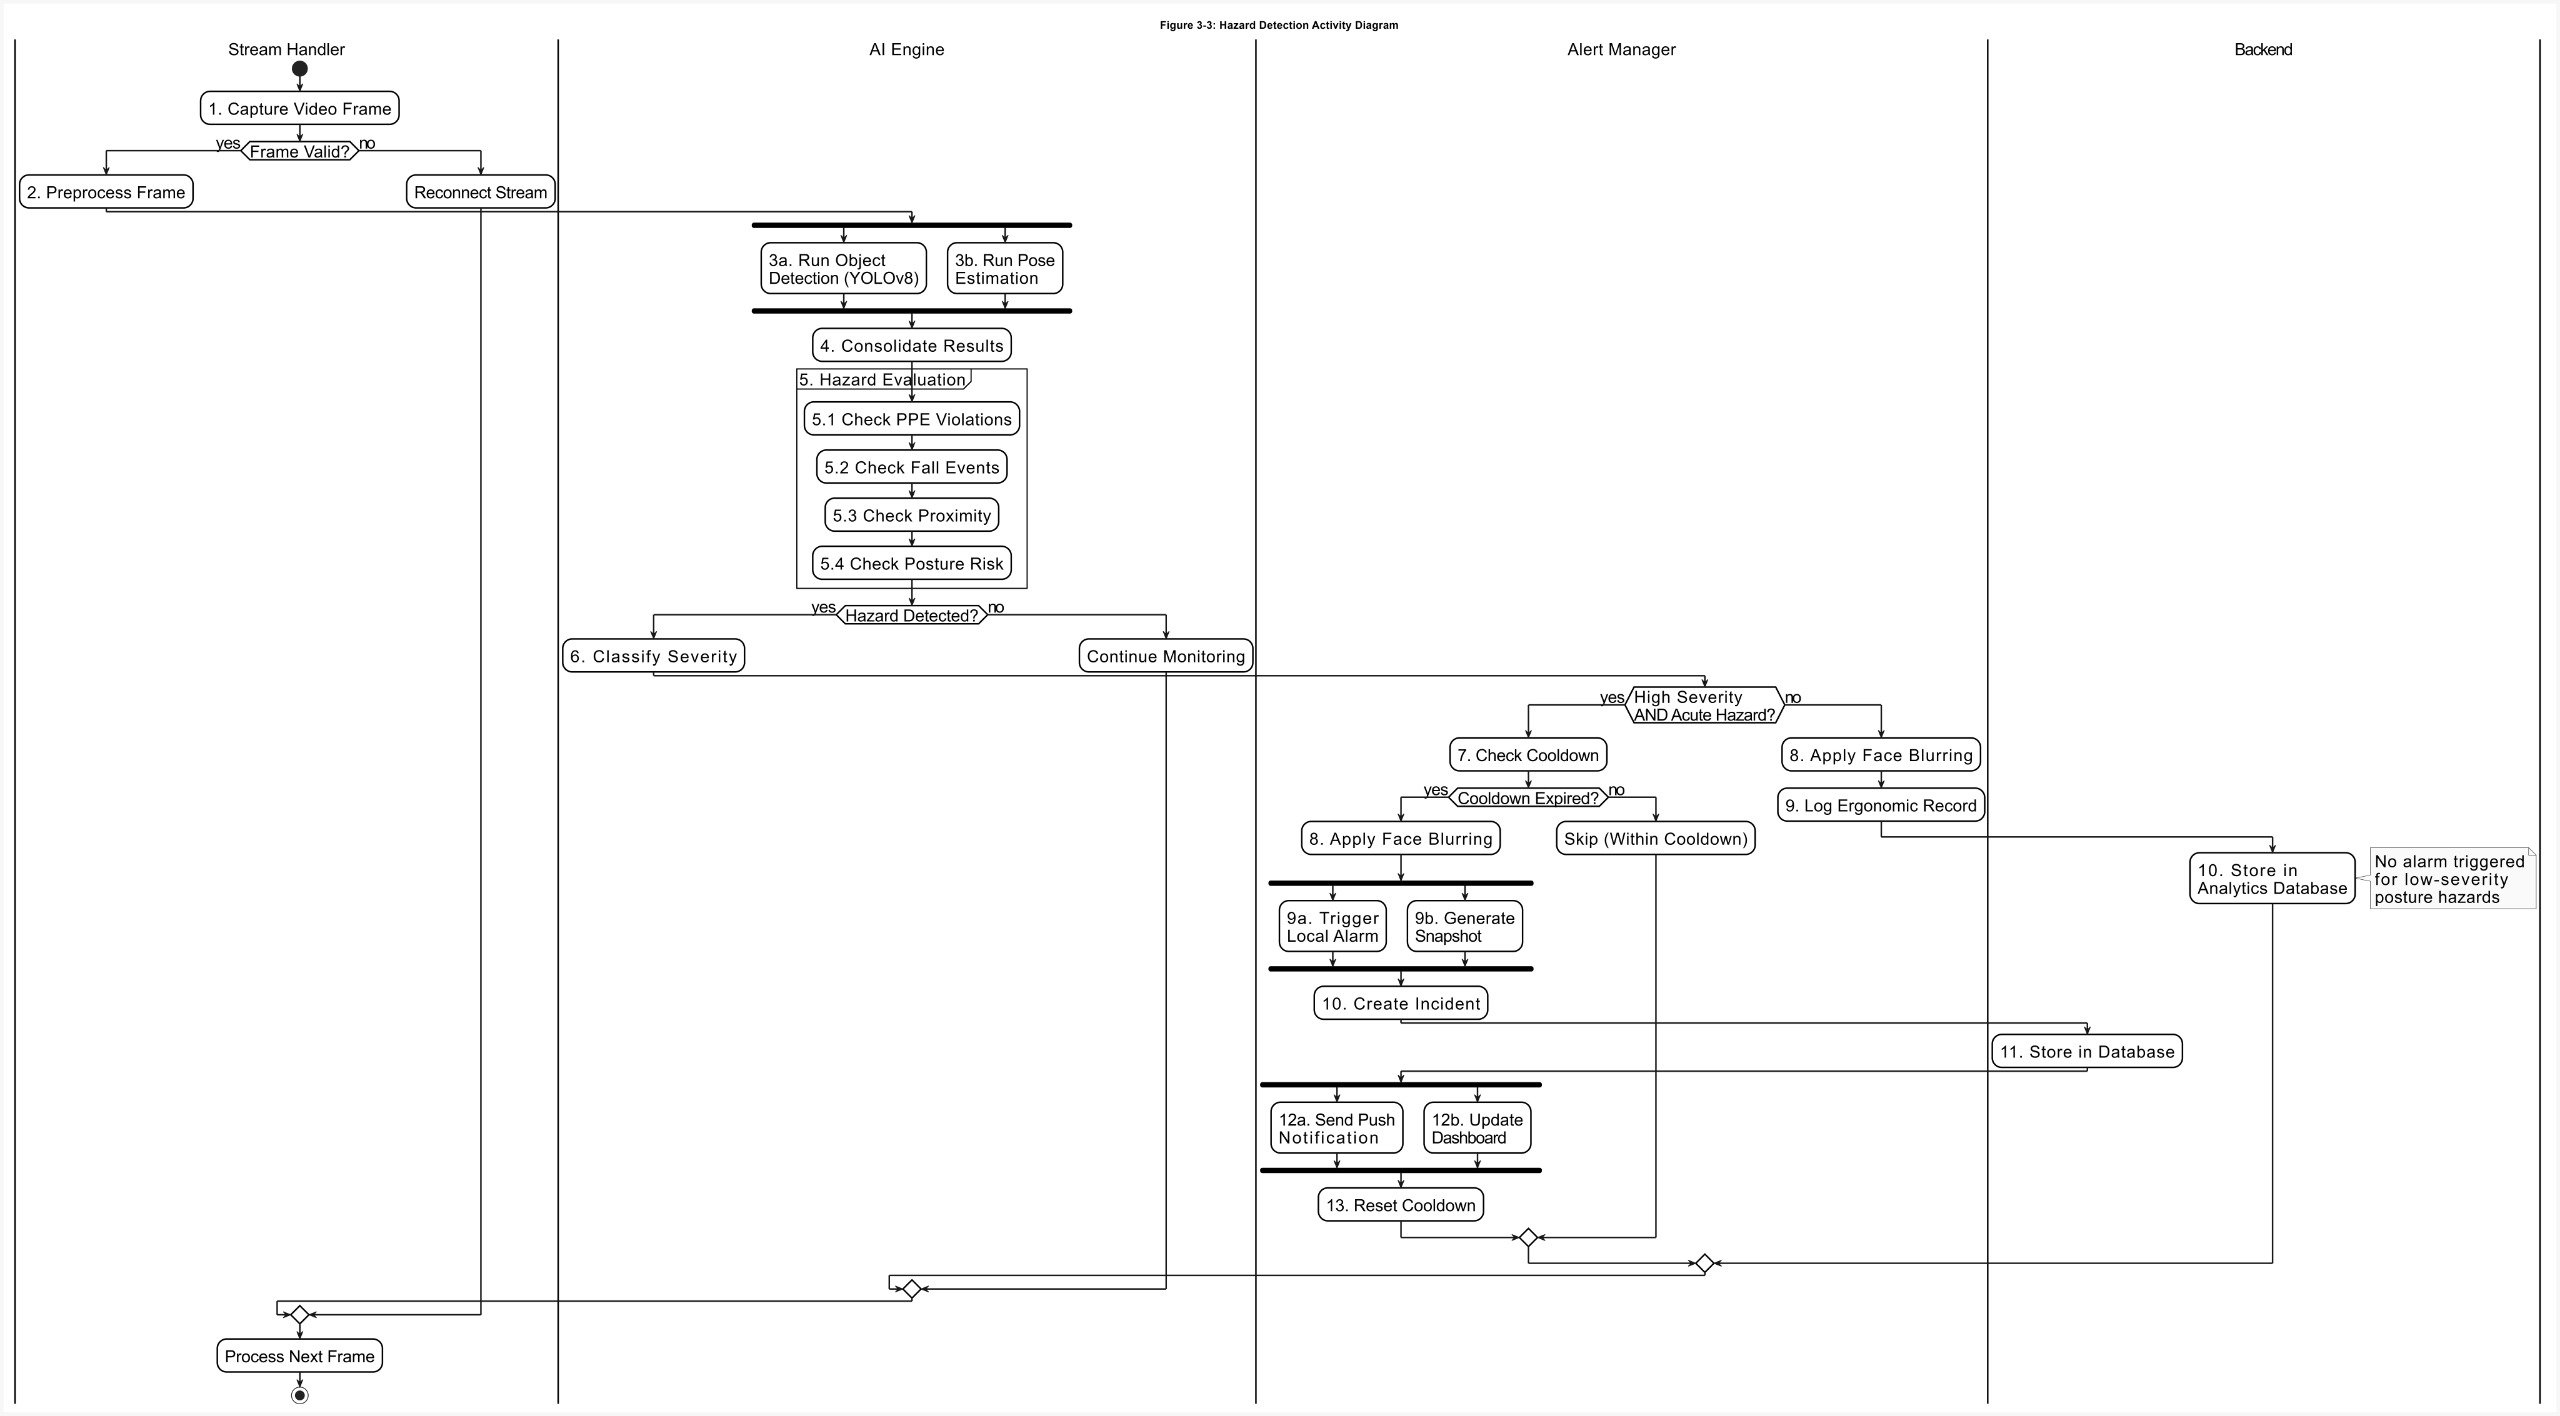
\includegraphics[width=0.95\linewidth,height=0.70\textheight,keepaspectratio]{images/img_017.jpeg}
\caption{System Architecture}
\end{figure}

\textbf{Component Roles and Interactions}

a. \textbf{Data Acquisition \& Processing:} Integrates camera feeds and AI models to detect safety breaches.

b. \textbf{Event Presentation Layer:} Translates system detections into human-readable summaries (type, severity, and location).

c. \textbf{Incident Lifecycle Manager:} Tracks events from the moment of detection through supervisor acknowledgement to final resolution.

d. \textbf{Analytics Engine:} Aggregates ergonomic and safety data into trend-based visual reports for long-term planning.

\section{Design Methodology}

The project utilizes an \textbf{Iterative, User-Centered Design (UCD) methodology}. This approach is essential for industrial safety systems where cognitive overload can lead to critical errors. The process involves repeated cycles of prototyping and refinement focusing on:

Information hierarchy and severity-based color coding.

Interface readability for control-room distances.

Mobile interaction efficiency for users in high-pressure field conditions.

Error prevention during high-impact actions like incident closure.

\section{Detailed Component Design}

The project design is modular, where each module corresponds to a distinct user task and interaction context:

\textbf{Monitoring Module (Web-centric):}

\textbf{Purpose:} Enables continuous scanning across multiple camera feeds.

\textbf{Design Details:} Features a stable grid layout, clear camera labeling, and a "Focus Mode" for high-priority streams.

\textbf{Emergency Incident Module (Dual-platform):}

\textbf{Purpose:} Surfaces urgent hazards requiring human intervention.

\textbf{Design Details:} Uses prominent visual cues (red/amber badges) and provides immediate access to incident snapshots.

\textbf{Incident Detail \& Evidence Module:}

\textbf{Purpose:} Supports quick confirmation and documentation of safety events.

\textbf{Design Details:} Displays anonymized evidence images, structured action logs, and a chronological timeline of the event lifecycle.

\textbf{Ergonomics Module (Preventive Analytics):}

\textbf{Purpose:} Supports the reduction of long-term musculoskeletal risks.

\textbf{Design Details:} Utilizes trend charts, exposure indicators, and zone-based heatmaps rather than intrusive alarms.

\section{UI/UX Design}

\textbf{A. Overview}

VisionSafe 360 delivers a unified experience where the \textbf{Web Dashboard} is optimized for investigation and the \textbf{Mobile App} is optimized for action. The design ensures consistent terminology, severity language, and navigation logic across both platforms.

\begin{figure}[H]
\centering
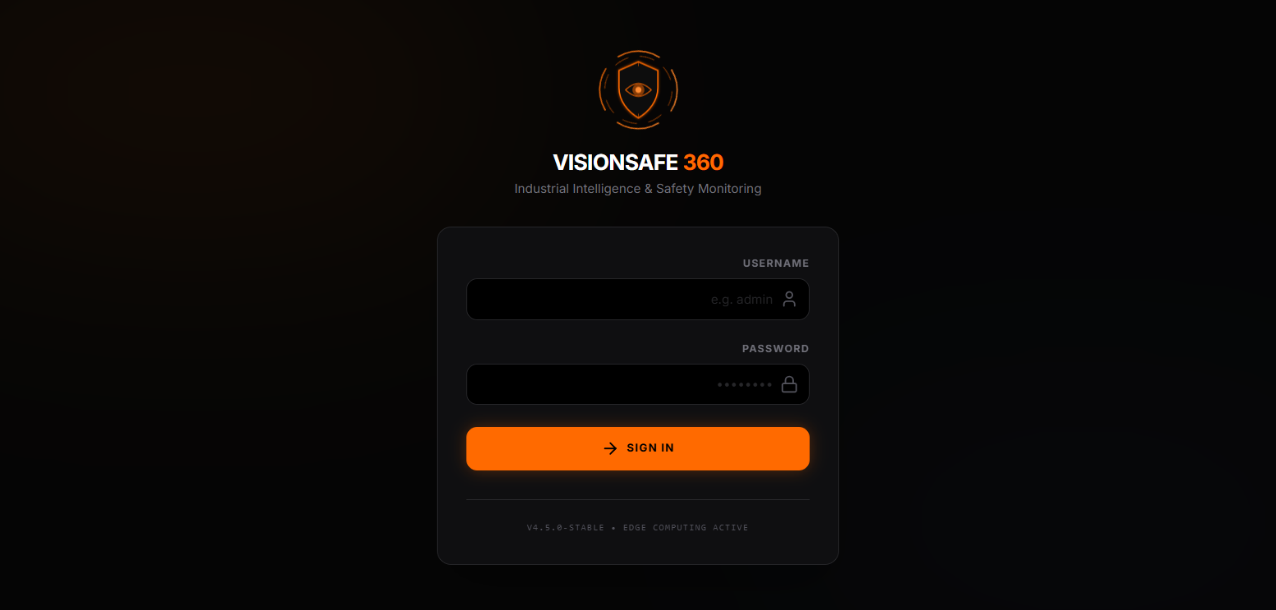
\includegraphics[width=0.95\linewidth,height=0.70\textheight,keepaspectratio]{images/img_018.png}
\caption{Web Dashboard Main Interface Layout}
\end{figure}

\begin{figure}[H]
\centering
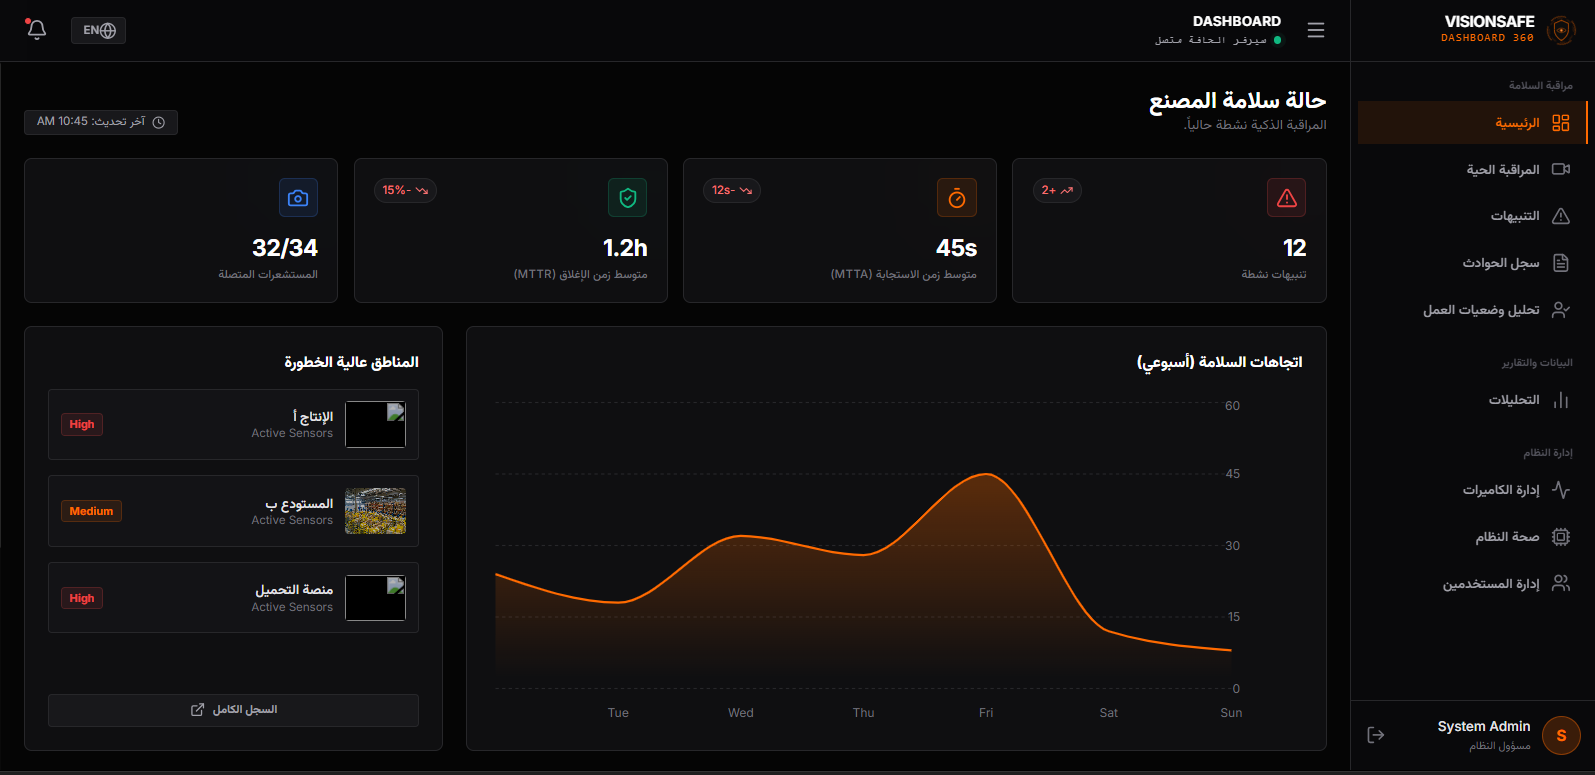
\includegraphics[width=0.95\linewidth,height=0.70\textheight,keepaspectratio]{images/img_019.png}
\caption{Web Dashboard Live Monitoring Interface}
\end{figure}

\begin{figure}[H]
\centering
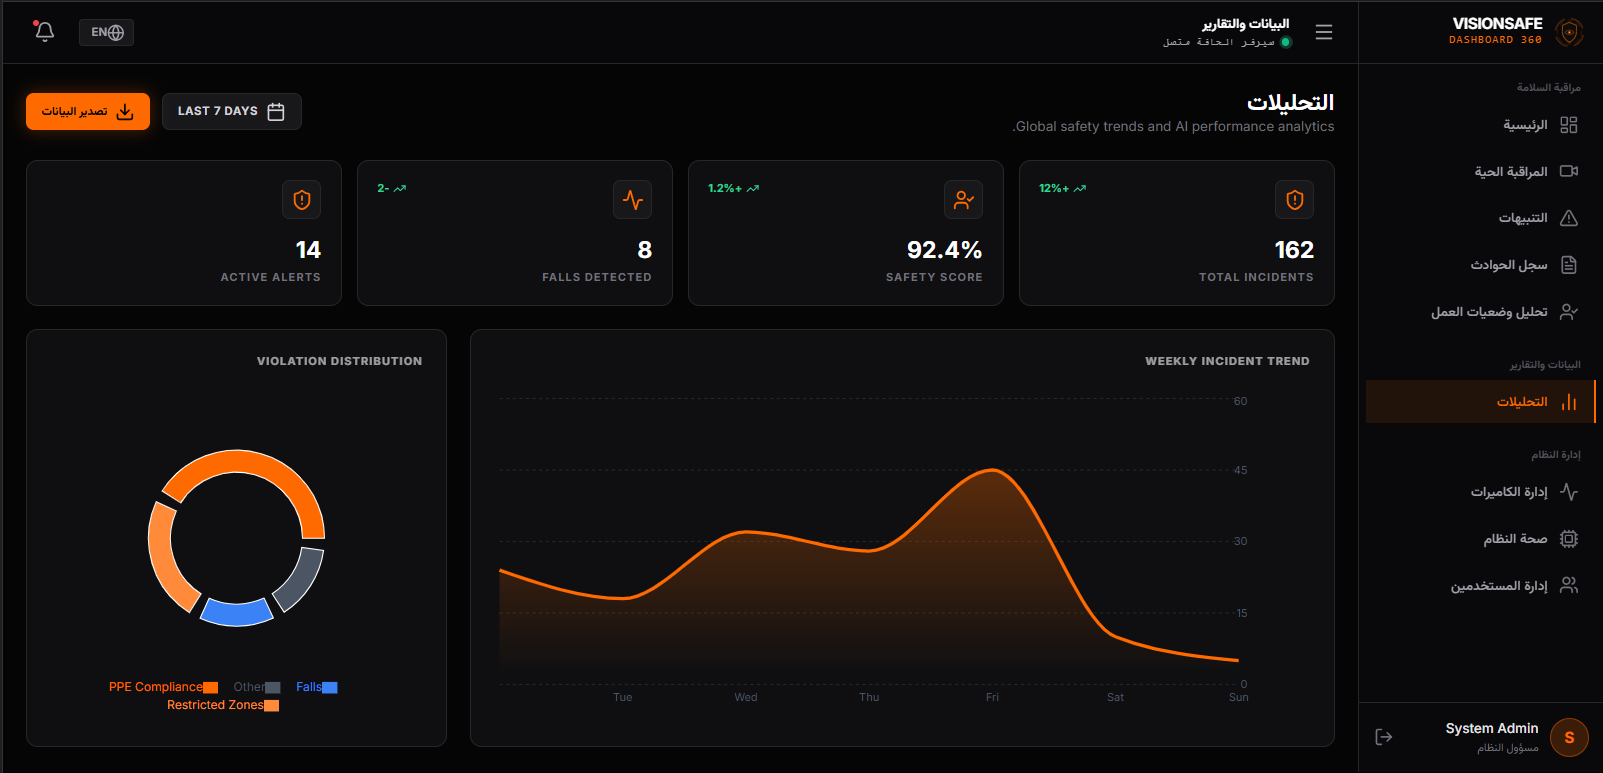
\includegraphics[width=0.95\linewidth,height=0.70\textheight,keepaspectratio]{images/img_020.png}
\caption{Web Dashboard Incident Interface}
\end{figure}

\begin{figure}[H]
\centering
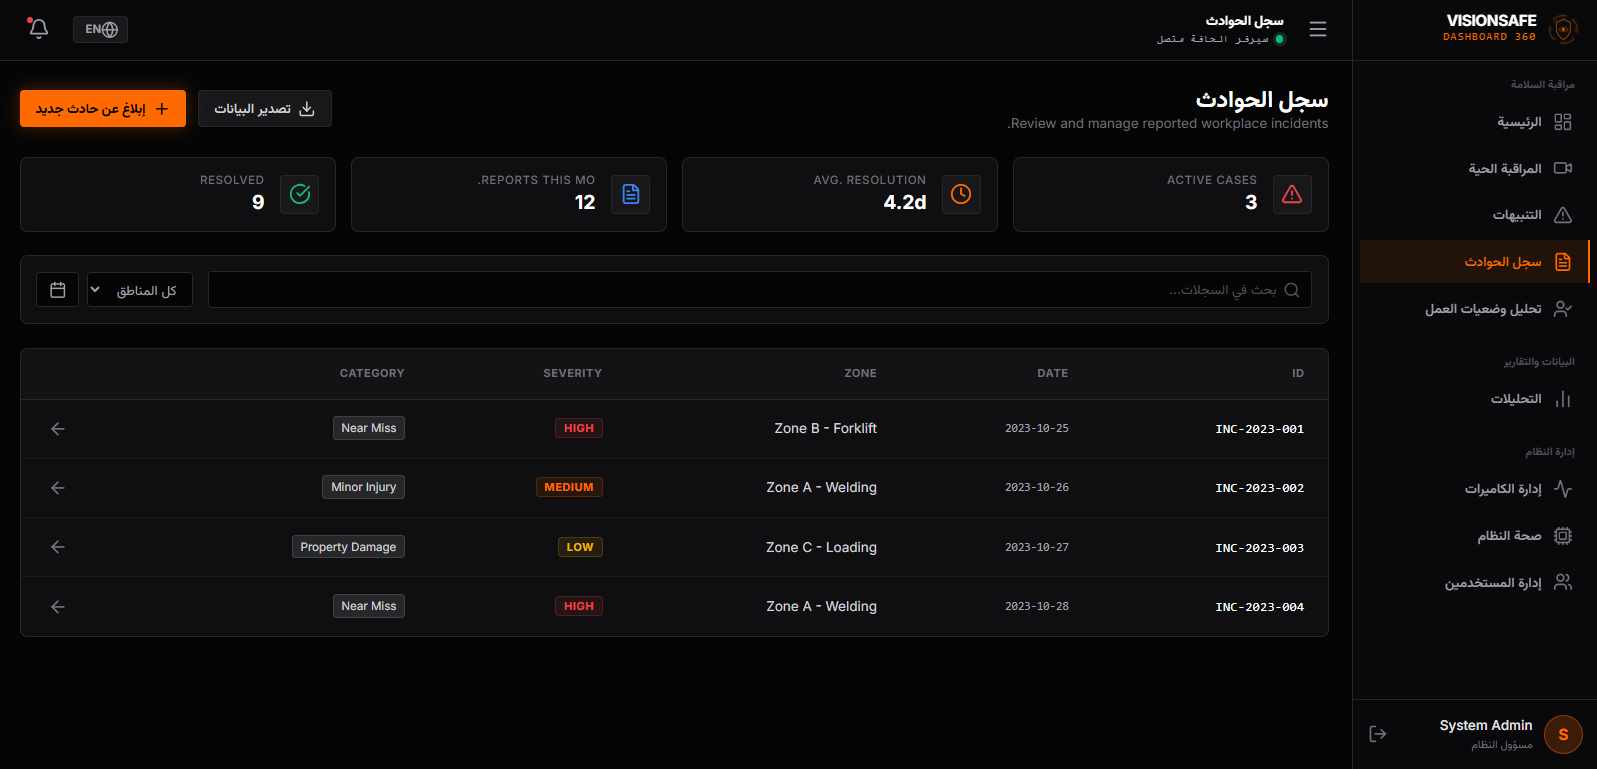
\includegraphics[width=0.95\linewidth,height=0.70\textheight,keepaspectratio]{images/img_021.png}
\caption{Web Dashboard Analytics Interface}
\end{figure}

\begin{figure}[H]
\centering
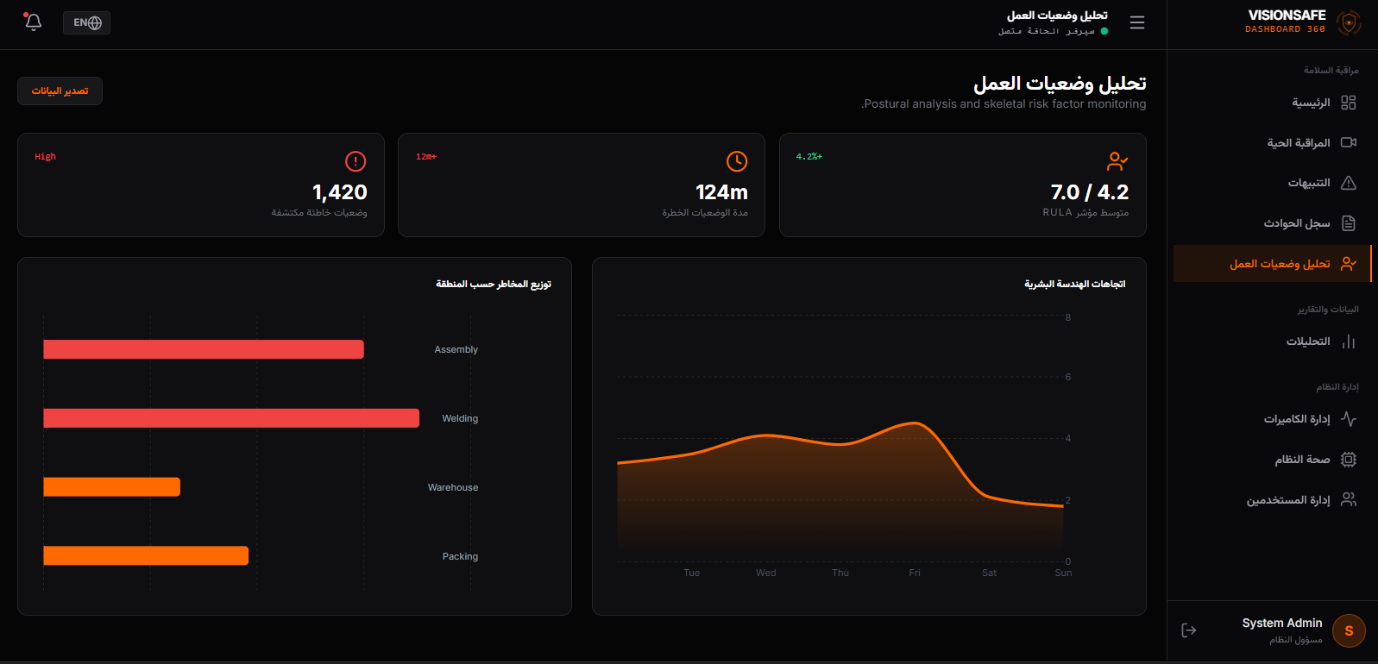
\includegraphics[width=0.95\linewidth,height=0.70\textheight,keepaspectratio]{images/img_022.png}
\caption{Web Dashboard Camera Management Interface}
\end{figure}

\begin{figure}[p]
\centering
\begin{minipage}[t]{0.45\linewidth}
	\centering
	
\includegraphics[height=0.34\textheight,keepaspectratio]{images/img_023.png}
	\captionof{figure}{Mobile Application Alert Overview}
\end{minipage}
\hfill
\begin{minipage}[t]{0.45\linewidth}
	\centering
	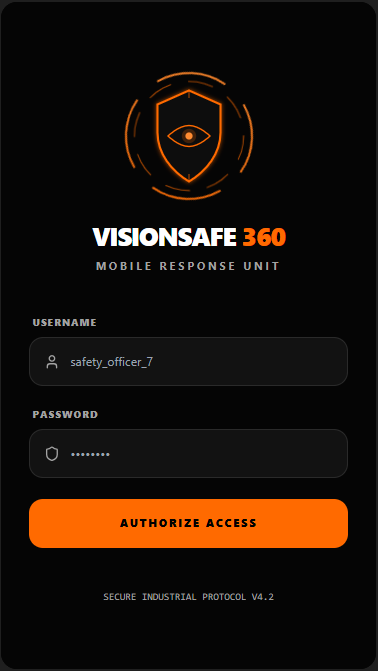
\includegraphics[height=0.34\textheight,keepaspectratio]{images/img_024.png}
	\captionof{figure}{Mobile Application Alert Details}
\end{minipage}

\vspace{0.8cm}
\begin{minipage}[t]{0.45\linewidth}
	\centering
	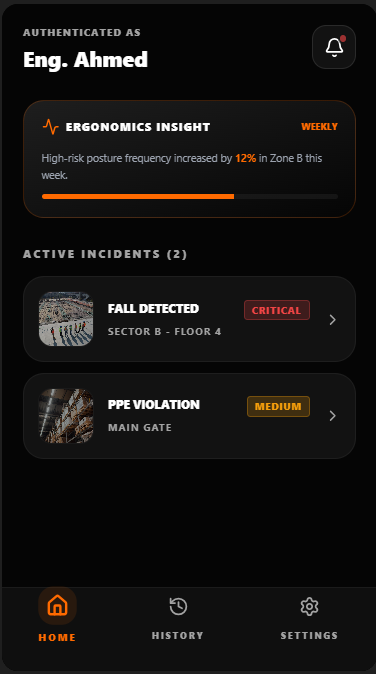
\includegraphics[height=0.34\textheight,keepaspectratio]{images/img_025.png}
	\captionof{figure}{Mobile Application Incident Acknowledgement}
\end{minipage}
\hfill
\begin{minipage}[t]{0.45\linewidth}
	\centering
	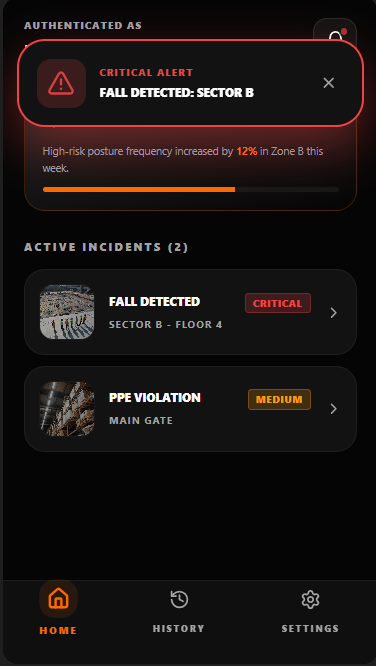
\includegraphics[height=0.34\textheight,keepaspectratio]{images/img_026.png}
	\captionof{figure}{Mobile Application Resolution Workflow}
\end{minipage}
\end{figure}

\begin{figure}[p]
\centering
\begin{minipage}[t]{0.45\linewidth}
	\centering
	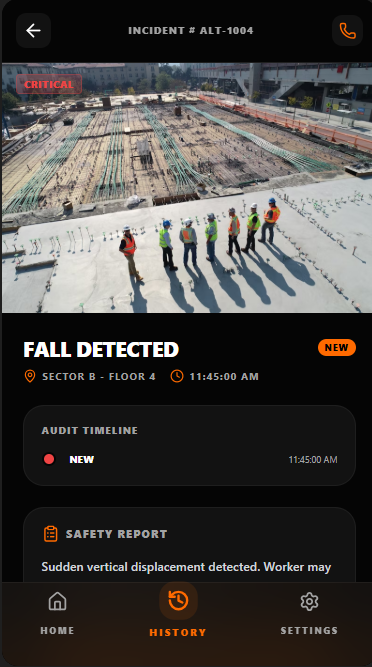
\includegraphics[height=0.34\textheight,keepaspectratio]{images/img_027.png}
	\captionof{figure}{Mobile Application Evidence View}
\end{minipage}
\hfill
\begin{minipage}[t]{0.45\linewidth}
	\centering
	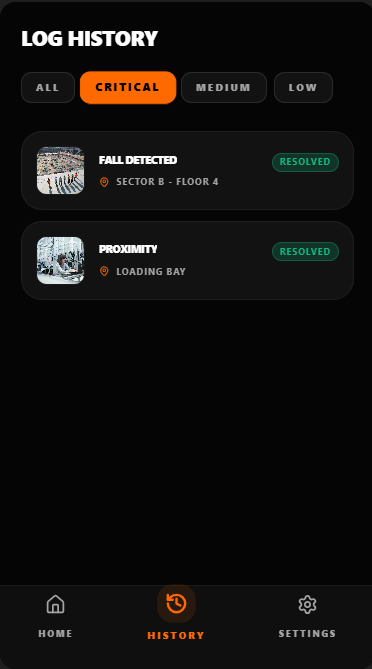
\includegraphics[height=0.34\textheight,keepaspectratio]{images/img_028.png}
	\captionof{figure}{Mobile Application Camera Status}
\end{minipage}

\vspace{0.8cm}
\begin{minipage}[t]{0.45\linewidth}
	\centering
	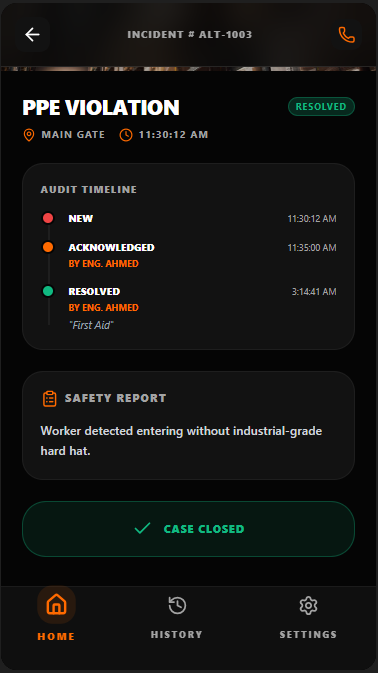
\includegraphics[height=0.34\textheight,keepaspectratio]{images/img_029.png}
	\captionof{figure}{Mobile Application Notifications}
\end{minipage}
\hfill
\begin{minipage}[t]{0.45\linewidth}
	\centering
	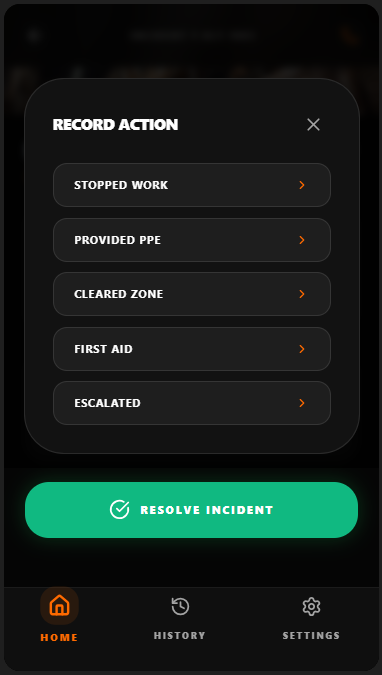
\includegraphics[height=0.34\textheight,keepaspectratio]{images/img_030.png}
	\captionof{figure}{Mobile Application Ergonomic Alert}
\end{minipage}
\end{figure}

\begin{figure}[p]
\centering
\begin{minipage}[t]{0.62\linewidth}
	\centering
	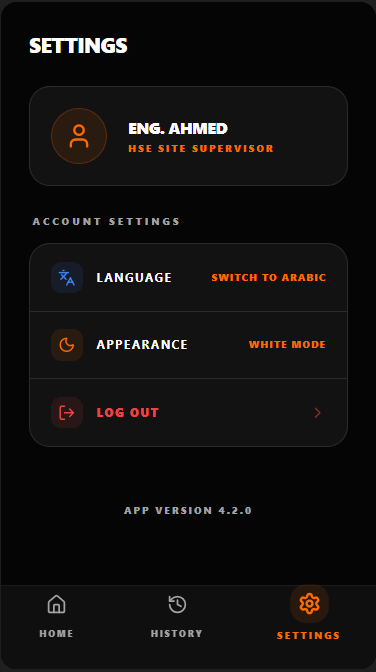
\includegraphics[height=0.60\textheight,keepaspectratio]{images/img_031.png}
	\captionof{figure}{Mobile Application Interface for Field Alerts}
\end{minipage}
\end{figure}

\textbf{B. User Interaction}

\textbf{The application ecosystem allows users to:}

Monitor multiple camera views and quickly focus on a specific feed.

Review emergency incidents with clear severity and location context.

Acknowledge incidents via mobile or web to confirm awareness and ownership.

Resolve incidents by recording corrective actions for audit purposes.

\textbf{Outputs are delivered through:}

\textbf{Incident Cards:} Summarizing type, severity, location, and timestamp.

\textbf{Visual Evidence:} Anonymized snapshots for rapid incident confirmation.

\textbf{Trend Dashboards:} Summary indicators and charts for long-term analysis.

\textbf{C. Design Principles}

\textbf{Simplicity:} Reducing cognitive load through clean layouts and minimal steps for critical actions.

\textbf{Clarity and Hierarchy:} Prioritizing urgent hazards while keeping secondary details available but not dominant.

\textbf{Accessibility:} High contrast, readable typography, and non-color-only severity cues (using icons and text).

\textbf{Error Prevention:} Confirmation dialogs for destructive actions and clear system-state indicators (e.g., offline camera).

\section{Workflow Design}

\textbf{A. Emergency Incident Workflow}

This workflow ensures that every detected hazard is accounted for by a human supervisor.

\textbf{Detection:} AI identifies a hazard and triggers an alert.

\textbf{Notification:} Alert appears on the Web Dashboard and the Mobile App simultaneously.

\textbf{Acknowledgement:} A supervisor confirms ownership via the mobile device.

\textbf{Resolution:} The supervisor records the corrective action taken to close the incident.

\textbf{B. Ergonomics Workflow}

\textbf{Passive Monitoring:} Ergonomic risks are logged as data points without immediate alarms.

\textbf{Trend Analysis:} HSE Managers review cumulative data on the Web Dashboard weekly/monthly.

\textbf{Strategic Intervention:} Decisions are made based on high-risk zones or recurring posture issues.

\section{Database Design (Conceptual)}

\textbf{A. Overview}

The database is structured to support the core UX requirements: traceability, accountability, and reporting. It ensures that data remains consistent across the Web and Mobile interfaces.

\textbf{B. Table Descriptions}

\textbf{Users \& Roles:} Manages identity and access scope (Admin, Manager, Supervisor).

\textbf{Cameras:} Stores camera metadata and location tagging for UI labeling.

\textbf{Incidents:} Core table tracking hazard types, severity, snapshots, and lifecycle status.

\textbf{Ergonomic Records:} Stores posture risk summaries and exposure indicators for analytics.

\textbf{Action Logs:} Maintains an audit trail for every acknowledgement and resolution action.

\begin{figure}[H]
\centering
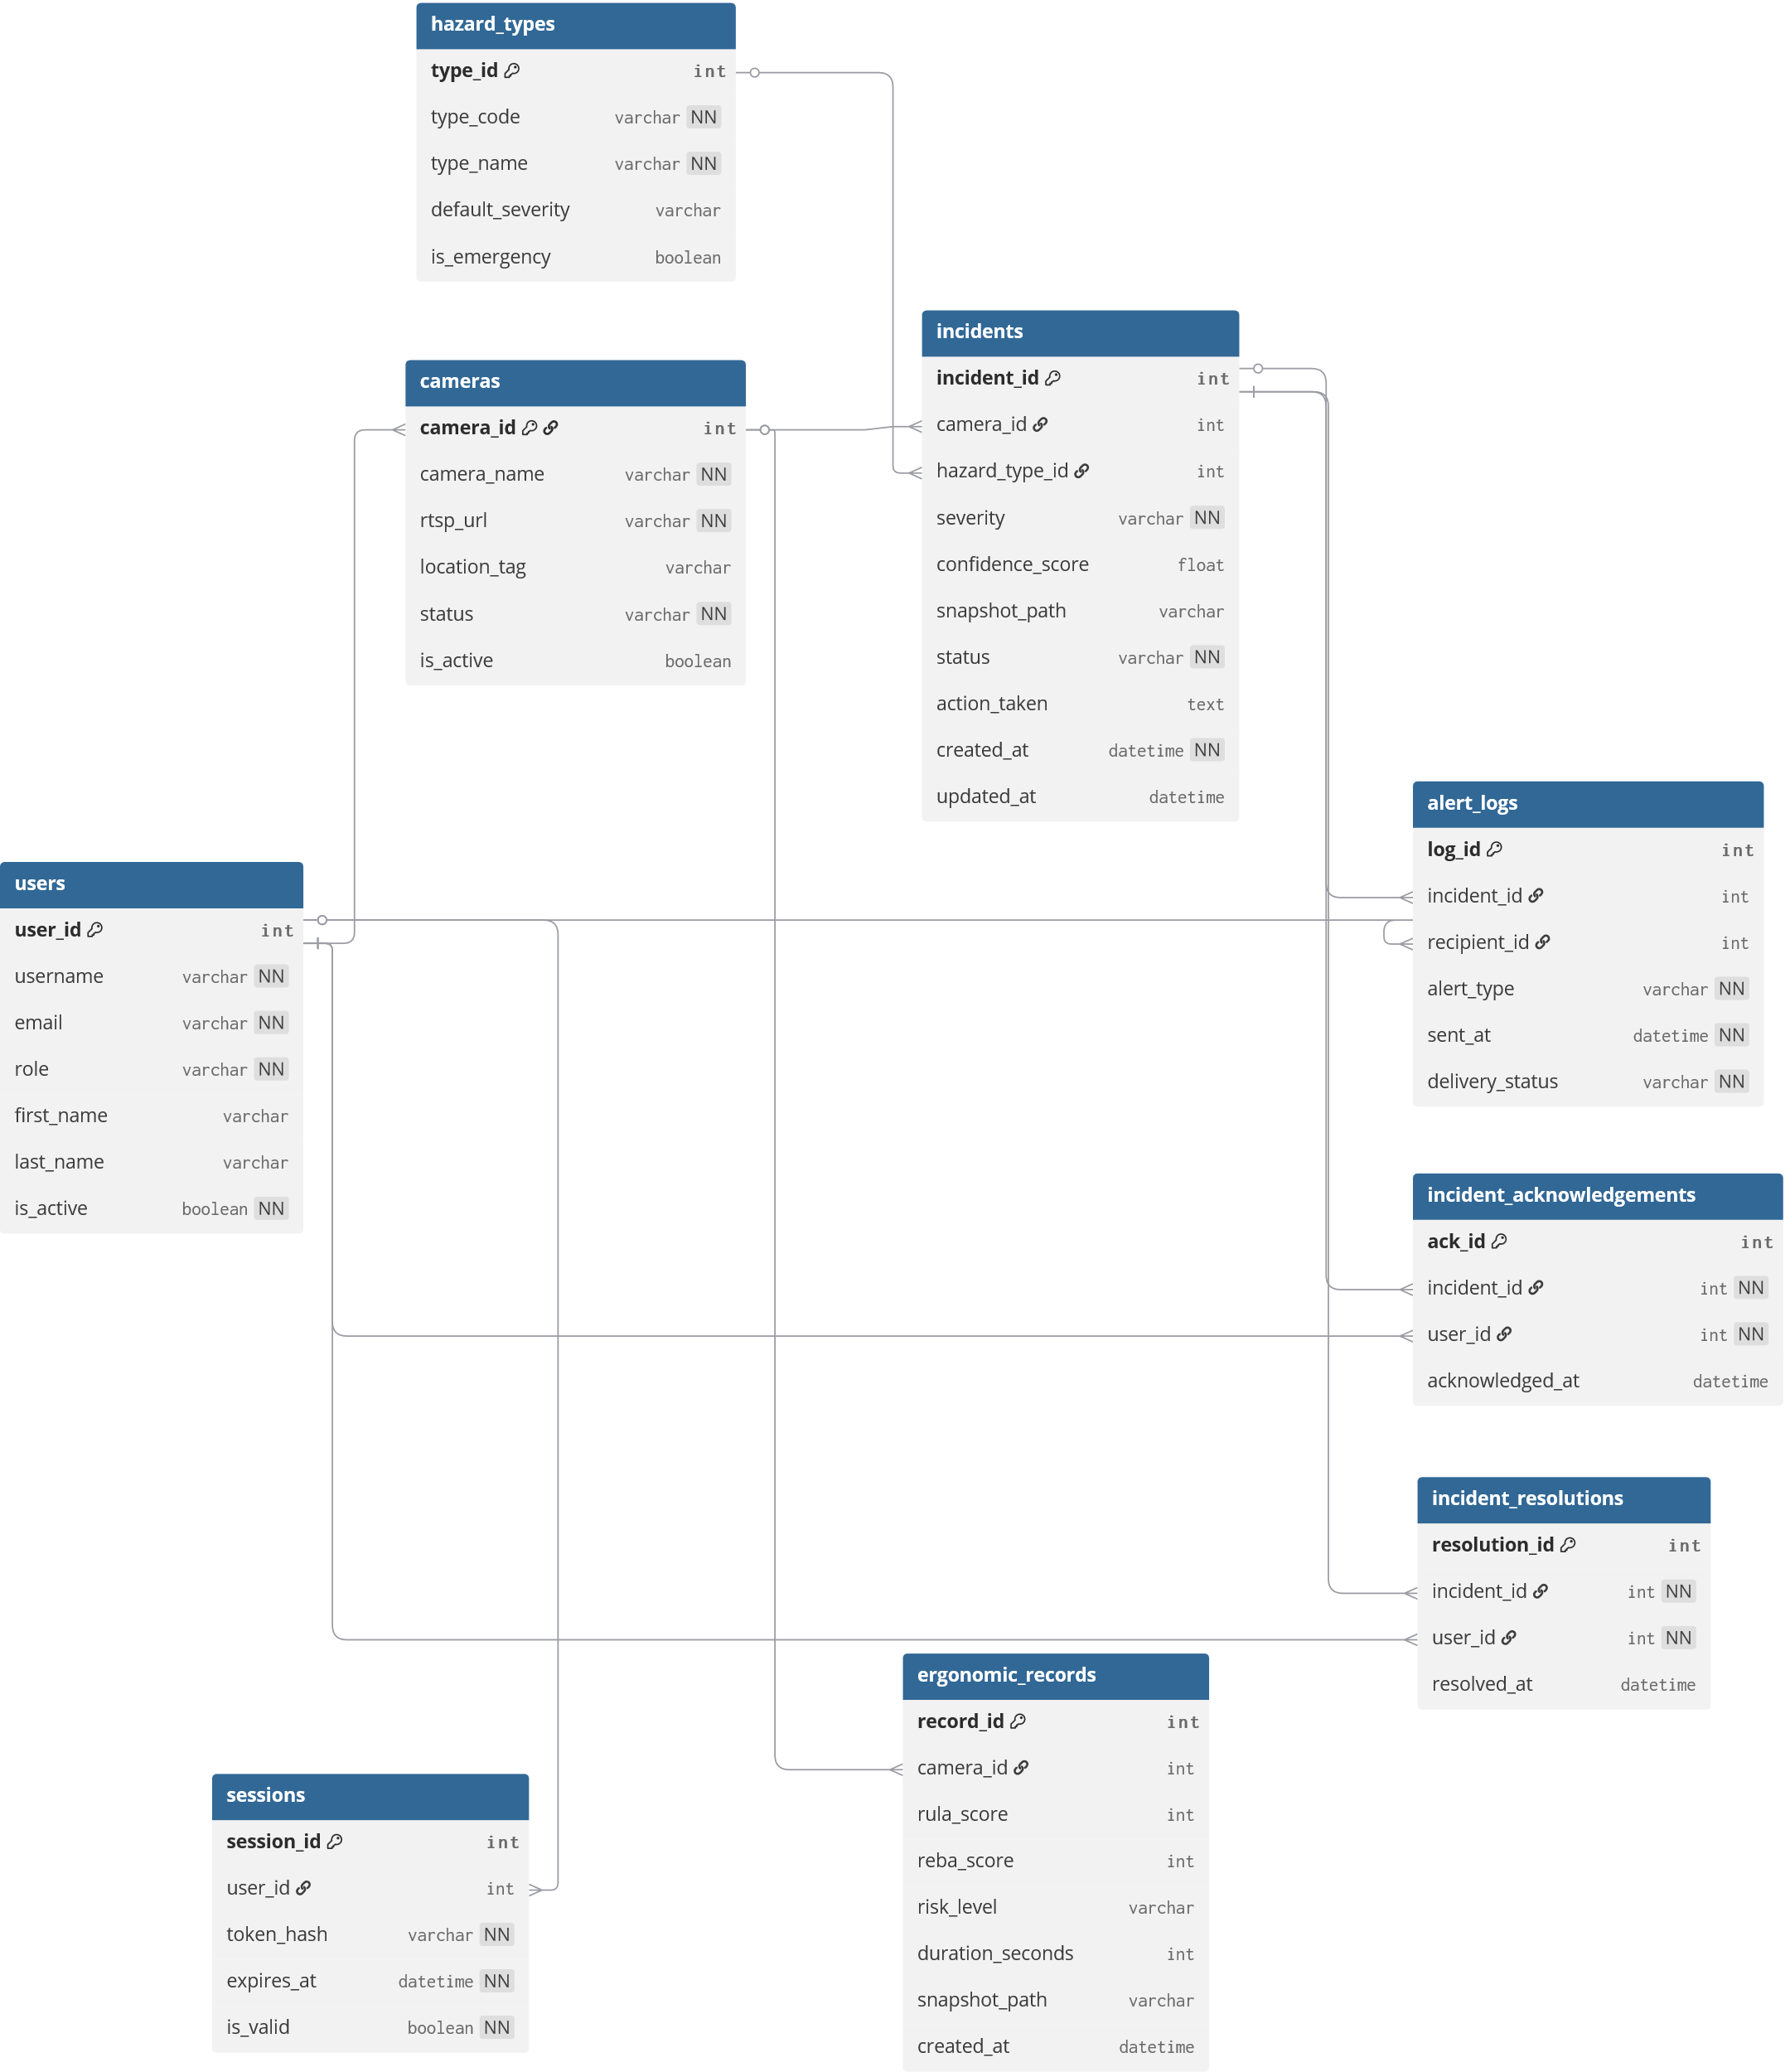
\includegraphics[width=0.95\linewidth,height=0.70\textheight,keepaspectratio]{images/img_032.png}
\caption{Entity-Relationship Diagram (ERD)}
\end{figure}

\section{Design Constraints}

a. \textbf{Operational Context:} Industrial environments introduce noise and distractions, requiring high-visibility UI.

b. \textbf{Monitoring Duration:} Visual design must minimize eye strain for control-room operators during long shifts.

c. \textbf{Device Diversity:} The design must remain usable on large desktop displays and ruggedized mobile screens.

d. \textbf{Privacy Requirements:} Evidence presentation must respect worker privacy through anonymization techniques.

\section{Rationale for Design Choices}

a. \textbf{Performance (UX):} The interface is structured to surface the most critical information first, reducing time-to-action.

b. \textbf{Platform Synergy:} Using the Web for "Heavy Data" (Analytics) and Mobile for "Fast Action" (Alerts) aligns with the natural professional behavior of safety officers.

c. \textbf{Scalability:} Consistent navigation and layout patterns remain usable as the number of monitored cameras increases.

\section{Integration of Avatars and Gesture Translation}

This section is not applicable to VisionSafe 360. The project scope is focused on industrial safety monitoring and incident workflows and does not involve avatar-based sign rendering or gesture translation.

\section{Backend and Application Development}

The application layer ensures that the user experience remains coherent across devices. The \textbf{Web Dashboard} is developed as a command hub for deep investigation, while the \textbf{Mobile Application} is designed as a field-oriented response tool. Both platforms communicate through a centralized backend that ensures real-time updates, predictable status transitions, and unified records, minimizing the need for manual synchronization or extensive operator training.

\chapter{Implementation}

\section{Implementation Overview}

This chapter explains how \textbf{VisionSafe360} was implemented as a complete AI-based workplace safety monitoring system. Unlike the design chapters, this chapter focuses on the practical implementation: the models that were loaded, the rules used to convert detections into hazards, the backend endpoints that receive incidents, and the dashboard mechanisms used to display live safety information.

The implemented system monitors video streams and detects four main hazard categories: missing personal protective equipment (PPE), unsafe worker--forklift proximity, worker falls, and harmful ergonomic posture. These modules run in an edge AI pipeline and send structured events to a FastAPI backend. The backend stores incidents, publishes real-time updates through WebSockets, and exposes data to the React dashboard.

\section{Development Milestones}

The implementation was completed in five main milestones. The first milestone defined the hazard categories and translated them into measurable computer vision tasks. PPE violations were represented as missing-equipment detections, forklift risk was represented as worker--vehicle distance, falls were represented as temporal posture transitions, and ergonomics were represented as RULA/REBA scores.

The second milestone focused on dataset preparation and model selection. YOLO-based models were selected for object detection and pose estimation because they provide real-time inference and integrated tracking support through the Ultralytics framework \cite{ultralytics_yolov8}.

The third milestone implemented the edge AI modules. Each hazard module was developed as a separate analyzer so that the pipeline could enable or disable PPE, proximity, fall, and posture logic independently.

The fourth milestone implemented the backend and dashboard. FastAPI was used for authenticated API endpoints, PostgreSQL was used for persistent records, Redis supported real-time event delivery and worker orchestration, and React/TypeScript was used for the dashboard interface.

The final milestone integrated the system using REST, WebSocket streams, and Docker Compose so that the prototype could run as a connected multi-service application.

\section{System Architecture Implementation}

VisionSafe360 was implemented as a layered architecture consisting of video input, edge AI processing, backend services, and dashboard visualization.

The \textbf{video input layer} receives frames from CCTV cameras, webcams, IP cameras, RTSP streams, or uploaded video files. The stream handler keeps only the latest frame when necessary so that processing remains close to real time instead of building a large queue of old frames.

\begin{figure}[H]
\centering
\safeincludegraphics[width=0.95\linewidth,height=0.55\textheight,keepaspectratio]{images/video_input_pipeline.png}
\caption{Video input pipeline}
\end{figure}

The \textbf{edge AI processing layer} owns the GPU inference loop. It loads the pose, PPE, and proximity models, performs YOLO inference, applies ByteTrack tracking where needed, and passes detections to the hazard analyzers.

\begin{figure}[H]
\centering
\safeincludegraphics[width=0.95\linewidth,height=0.55\textheight,keepaspectratio]{images/edge_ai_pipeline.png}
\caption{Edge AI processing pipeline}
\end{figure}

The \textbf{backend layer} receives incidents from edge workers, validates requests, stores records, applies rate limits, and broadcasts incident updates to connected dashboard clients.

The \textbf{dashboard layer} provides live monitoring, incident management, alerts, reports, camera management, ergonomics analytics, and system configuration.

\begin{figure}[H]
\centering
\safeincludegraphics[width=0.95\linewidth,height=0.60\textheight,keepaspectratio]{images/fig_5_3_complete_architecture.png}
\caption{Complete VisionSafe360 architecture}
\end{figure}

\section{Technologies and Tools Used}

Table~\ref{tab:chapter5-technologies} summarizes the main tools used in the implementation. Version numbers were taken from the project requirements and package configuration files.

\begin{table}[H]
\centering
\footnotesize
\renewcommand{\arraystretch}{1.45}
\begin{tabular}{|p{0.2\linewidth}|p{0.16\linewidth}|p{0.28\linewidth}|p{0.25\linewidth}|}
\hline
\textbf{Tool} & \textbf{Version} & \textbf{Purpose} & \textbf{Justification} \\
\hline
Python & 3.11 & Edge AI and backend services & Strong AI and API ecosystem \\
\hline
Ultralytics YOLO & 8.4.16 & Detection, pose estimation, and tracking & Real-time model execution and ByteTrack integration \\
\hline
PyTorch & 2.10.0 + CUDA 12.8 & GPU inference & Efficient tensor execution on NVIDIA GPU \\
\hline
OpenCV & 4.13.0 / 4.10.0 & Frame handling and image processing & Mature video processing library \\
\hline
FastAPI & 0.115.0 & Backend REST API and WebSocket routing & Fast asynchronous API framework \cite{fastapi_docs} \\
\hline
PostgreSQL & 16 & Persistent database & Reliable relational storage \cite{postgres_docs} \\
\hline
SQLAlchemy & 2.0.35 & ORM/database layer & Structured database models and migrations \\
\hline
Redis & 5.0.8 client, Redis 7 services & Queues, rate counters, event streams, latest-frame cache & Low-latency shared state and Pub/Sub \cite{redis_docs} \\
\hline
React & 19.2.1 & Dashboard UI & Component-based interface development \cite{react_docs} \\
\hline
TypeScript & 5.8.2 & Dashboard application logic & Type safety for frontend data models \\
\hline
Tailwind CSS & 3.4.4 & Dashboard styling & Consistent utility-first UI styling \\
\hline
Docker Compose & Compose stack & Multi-service deployment & Reproducible backend, dashboard, database, Redis, and worker services \cite{docker_compose_docs} \\
\hline
\end{tabular}
\caption{\textbf{Technologies and tools used in VisionSafe360}}
\label{tab:chapter5-technologies}
\end{table}

\section{Hardware Environment}

The project was developed and tested on a laptop with GPU acceleration. The hardware was sufficient for running YOLO inference, backend services, and the dashboard during prototype testing.

\begin{table}[H]
\centering
\renewcommand{\arraystretch}{1.55}
\begin{tabular}{|>{\centering\arraybackslash}p{0.3\linewidth}|>{\centering\arraybackslash}p{0.58\linewidth}|}
\hline
\textbf{Component} & \textbf{Specification} \\
\hline
\textbf{CPU} & Intel Core i5-13420H \\
\hline
\textbf{GPU} & NVIDIA GeForce RTX 4050 Laptop GPU \\
\hline
\textbf{RAM} & 16 GB \\
\hline
\textbf{Operating System} & Windows 11 development environment \\
\hline
\end{tabular}
\caption{\textbf{Hardware environment used for development and testing}}
\label{tab:chapter5-hardware}
\end{table}

\section{Module Implementation}

The edge AI implementation is divided into independent modules. Each module receives detections or pose keypoints and returns a list of structured hazard events. This modular design makes the system easier to test and allows specific hazards to be enabled through runtime profiles.

\subsection{PPE Detection}

The PPE detection module monitors whether workers are wearing required equipment such as helmets, safety vests, gloves, and safety shoes. The module uses a YOLO model trained on SH17, a public PPE dataset containing 8,099 images and 75,994 labeled instances across 17 classes \cite{ahmad2024sh17}. In the implementation, SH17-style labels are normalized into application labels such as \texttt{helmet\_on}, \texttt{helmet\_off}, \texttt{safety\_vest}, \texttt{vest\_off}, \texttt{gloves\_off}, and \texttt{bare\_foot}.

\begin{table}[H]
\centering
\renewcommand{\arraystretch}{1.45}
\begin{tabular}{|>{\centering\arraybackslash}p{0.32\linewidth}|>{\centering\arraybackslash}p{0.56\linewidth}|}
\hline
\textbf{Item} & \textbf{Value} \\
\hline
\textbf{Dataset} & SH17 PPE Dataset \\
\hline
\textbf{Images / Instances} & 8,099 images / 75,994 instances \\
\hline
\textbf{Detected PPE Classes} & Helmet, safety vest, gloves, shoes, mask, glasses, face guard, ear protection, suit, tool, and related missing-equipment classes \\
\hline
\textbf{Input Resolution} & 640$\times$640 \\
\hline
\textbf{Model Family} & YOLO detector \\
\hline
\textbf{Persistence Rule} & Missing PPE must persist before an incident is emitted \\
\hline
\end{tabular}
\caption{\textbf{PPE dataset and implementation configuration}}
\label{tab:chapter5-ppe-dataset}
\end{table}

Listing~\ref{lst:ppe-inference} shows the core PPE inference pattern. The model is loaded once, then each frame is passed to YOLO with confidence, IoU, and maximum-detection limits.

\begin{lstlisting}[language=Python,caption={PPE model inference on one frame},label={lst:ppe-inference}]
from ultralytics import YOLO

ppe_model = YOLO("weights/ppe/best_ppe.pt")

results = ppe_model.predict(
    frame,
    device="cuda:0",
    imgsz=640,
    conf=0.30,
    iou=0.50,
    max_det=100,
    verbose=False,
)[0]

detections = []
for box in results.boxes:
    cls_id = int(box.cls[0])
    name = ppe_model.names[cls_id].lower()
    detections.append((name, float(box.conf[0]), box.xyxy[0]))
\end{lstlisting}

The analyzer converts missing-equipment detections into hazard events. For example, \texttt{helmet\_off} is converted into a high-severity missing-helmet event, while \texttt{gloves\_off} is treated as medium severity. The event aggregator then applies persistence and cooldown logic to reduce false positives caused by short occlusions.

\begin{figure}[H]
\centering
\safeincludegraphics[width=0.95\linewidth,height=0.58\textheight,keepaspectratio]{images/Vest, Helmet, Gloves detection.png}
\caption{PPE detection output}
\end{figure}

\subsection{Forklift Proximity Detection}

The forklift proximity module detects unsafe distances between workers and forklifts. The implementation uses a YOLO detector for forklifts and persons, then calculates Euclidean distance between bounding box centroids in pixel space. The current prototype uses pixel thresholds because monocular CCTV footage does not provide direct depth information. Camera calibration can later replace these pixel thresholds with meter-based distances.

\begin{table}[H]
\centering
\renewcommand{\arraystretch}{1.45}
\begin{tabular}{|>{\centering\arraybackslash}p{0.34\linewidth}|>{\centering\arraybackslash}p{0.54\linewidth}|}
\hline
\textbf{Item} & \textbf{Value} \\
\hline
\textbf{Model} & YOLOv8m forklift/person detector \\
\hline
\textbf{Training Images} & 2,468 \\
\hline
\textbf{Validation Images} & 500 \\
\hline
\textbf{Epochs / Batch Size} & 200 epochs / batch size 16 \\
\hline
\textbf{Danger Threshold} & 80 pixels \\
\hline
\textbf{Warning Threshold} & 140 pixels \\
\hline
\textbf{Alert Persistence} & Unsafe proximity must persist for approximately one second \\
\hline
\end{tabular}
\caption{\textbf{Forklift proximity model and rule configuration}}
\label{tab:chapter5-forklift-model}
\end{table}

Listing~\ref{lst:proximity} shows the core rule. The nearest forklift is selected for each person, and severity is assigned based on the configured danger and warning radii.

\begin{lstlisting}[language=Python,caption={Worker--forklift distance check},label={lst:proximity}]
def center(bbox):
    x1, y1, x2, y2 = bbox
    return ((x1 + x2) / 2.0, (y1 + y2) / 2.0)

def distance_px(a, b):
    ax, ay = center(a)
    bx, by = center(b)
    return ((ax - bx) ** 2 + (ay - by) ** 2) ** 0.5

for person in persons:
    dist_px, forklift = min(
        (distance_px(person.bbox, f.bbox), f) for f in forklifts
    )
    if dist_px <= 80:
        emit_event("forklift_proximity_danger", "High", person)
    elif dist_px <= 140:
        emit_event("forklift_proximity_warning", "Medium", person)
\end{lstlisting}

\begin{figure}[H]
\centering
\safeincludegraphics[width=0.95\linewidth,height=0.58\textheight,keepaspectratio]{images/Forklift and worker detection.png}
\caption{Forklift detection output}
\end{figure}

\subsection{Fall Detection}

The fall detection module uses a pose-aware rule engine rather than a heavy sequence model. This decision reduced computational cost and made the system easier to explain and tune. Each tracked person has an independent state machine with three implementation states: \texttt{normal}, \texttt{candidate}, and \texttt{confirmed}. A recovered posture returns the track to \texttt{normal}.

The system evaluates bounding box aspect ratio, downward centroid velocity, hip position from COCO keypoints, and immobility. A fall is confirmed only after the candidate posture persists for 2.5 seconds, reducing false alarms from bending, crouching, or short occlusions.

\begin{lstlisting}[language=Python,caption={Fall state transition logic},label={lst:fall-state}]
if state == "normal" and triggered:
    state = "candidate"
    candidate_since = timestamp

elif state == "candidate":
    recovered = hip_ratio > 0.6 if hip_ratio else aspect_ratio < 0.8
    if recovered:
        state = "normal"
    elif timestamp - candidate_since >= 2.5:
        state = "confirmed"
        emit_event(
            "fall_confirmed",
            severity="Critical",
            metadata={"aspect_ratio": aspect_ratio,
                      "hip_ratio": hip_ratio},
        )

elif state == "confirmed" and recovered:
    state = "normal"
\end{lstlisting}

\begin{figure}[H]
\centering
\safeincludegraphics[width=0.95\linewidth,height=0.58\textheight,keepaspectratio]{images/fig_5_7_fall_state_machine.png}
\caption{Fall detection state machine}
\end{figure}

\begin{figure}[H]
\centering
\safeincludegraphics[width=0.95\linewidth,height=0.58\textheight,keepaspectratio]{images/Fallen worker .png}
\caption{Fall detection alert}
\end{figure}

\subsection{Ergonomic Posture Analysis}

The ergonomic posture module computes body angles from COCO-17 pose keypoints and feeds them into RULA and REBA scoring functions \cite{mcatamney1993rula,hignett2000reba}. Joint angles are derived from keypoint groups. For example, trunk flexion is computed from the midpoint between both hips and the midpoint between both shoulders, while upper-arm and lower-arm angles use shoulder, elbow, wrist, and hip keypoints.

\begin{table}[H]
\centering
\renewcommand{\arraystretch}{1.55}
\begin{tabular}{|>{\centering\arraybackslash}p{0.34\linewidth}|>{\centering\arraybackslash}p{0.54\linewidth}|}
\hline
\textbf{Metric} & \textbf{Threshold} \\
\hline
\textbf{RULA Alert} & $\geq$ 5 \\
\hline
\textbf{REBA Alert} & $\geq$ 7 \\
\hline
\textbf{Critical Risk} & RULA = 7 or REBA $\geq$ 11 \\
\hline
\textbf{Sustained Poor Posture} & 4 seconds before event emission \\
\hline
\textbf{Smoothing} & Exponential moving average with alpha = 0.6 \\
\hline
\end{tabular}
\caption{\textbf{Ergonomic posture alert thresholds}}
\label{tab:chapter5-ergonomic-thresholds}
\end{table}

Listing~\ref{lst:angle} shows the angle calculation used by the ergonomics implementation. The function computes the angle at a joint by comparing the vectors connected to that joint.

\begin{lstlisting}[language=Python,caption={Joint angle calculation for RULA/REBA},label={lst:angle}]
def angle_between(a, b, c):
    ba = a - b
    bc = c - b
    norm_ba = np.linalg.norm(ba)
    norm_bc = np.linalg.norm(bc)
    if norm_ba < 1e-6 or norm_bc < 1e-6:
        return None
    cos_angle = np.dot(ba, bc) / (norm_ba * norm_bc)
    cos_angle = np.clip(cos_angle, -1.0, 1.0)
    return float(np.degrees(np.arccos(cos_angle)))

angles = compute_angles(smoothed_keypoints, confidences)
rula_score = compute_rula(angles)["final_score"]
reba_score = compute_reba(angles)["final_score"]
\end{lstlisting}

\begin{figure}[H]
\centering
\safeincludegraphics[width=0.95\linewidth,height=0.58\textheight,keepaspectratio]{images/posture skeleton.png}
\caption{Posture skeleton detection}
\end{figure}

\subsection{Tracking and Event Persistence}

Tracking is used to maintain worker identity across frames and prevent duplicate incidents. The implementation uses Ultralytics \texttt{model.track(...)} with ByteTrack. The tracker provides persistent \texttt{track\_id} values that are passed to the PPE, proximity, fall, and ergonomics modules.

\begin{lstlisting}[language=Python,caption={ByteTrack initialization and ID assignment},label={lst:tracking}]
results = pose_model.track(
    frame,
    device="cuda:0",
    imgsz=640,
    conf=0.38,
    iou=0.50,
    tracker="bytetrack.yaml",
    persist=True,
    verbose=False,
)[0]

for box in results.boxes:
    track_id = int(box.id[0]) if box.id is not None else None
    detections.append(Detection(
        class_name="person",
        confidence=float(box.conf[0]),
        bbox=tuple(map(int, box.xyxy[0])),
        track_id=track_id,
    ))
\end{lstlisting}

Event persistence is handled by temporal rules. PPE events must remain visible before being reported, proximity events are emitted only when the threshold condition persists, fall events require a candidate confirmation window, and posture events require sustained high ergonomic risk. This design prevents single-frame errors from becoming incidents.

\section{Backend Implementation}

The backend was developed using FastAPI \cite{fastapi_docs}. It acts as the central communication layer for incidents, alerts, analytics, camera configuration, authentication, jobs, and real-time streams.

\begin{table}[H]
\centering
\footnotesize
\renewcommand{\arraystretch}{1.35}
\begin{tabular}{|p{0.24\linewidth}|p{0.24\linewidth}|p{0.41\linewidth}|}
\hline
\textbf{Endpoint Group} & \textbf{Method} & \textbf{Purpose} \\
\hline
\texttt{/api/incidents} & GET/POST/PATCH/DELETE & List, create, update, and delete incident records \\
\hline
\texttt{/api/alerts} & GET/POST/PATCH & Manage alert records and acknowledgement workflow \\
\hline
\texttt{/api/analytics/*} & GET & Provide time-series, severity, zone, and dashboard analytics \\
\hline
\texttt{/api/cameras} & GET/POST/PATCH/DELETE & Manage camera sources and metadata \\
\hline
\texttt{/api/ergonomics} & GET/POST & Store and query ergonomic score samples \\
\hline
\texttt{/api/jobs} & GET/POST & Start and monitor AI processing jobs \\
\hline
\texttt{/ws/incidents} & WebSocket & Push incident updates to dashboard clients \\
\hline
\texttt{/ws/stream/\{camera\_id\}} & WebSocket & Stream annotated AI frames to the dashboard \\
\hline
\end{tabular}
\caption{\textbf{Backend endpoint overview}}
\label{tab:chapter5-api}
\end{table}

The database layer uses SQLAlchemy models for incidents, alerts, cameras, users, notifications, ergonomic records, and system configuration. Alembic migrations are included to create and evolve the PostgreSQL schema. Redis is used for rate limiting, event Pub/Sub, worker queues, orchestration state, and latest-frame streaming.

Listing~\ref{lst:incident-endpoint} shows the core incident ingestion endpoint. After creating a database record, the backend broadcasts an \texttt{incident\_created} event to connected dashboard clients.

\begin{lstlisting}[language=Python,caption={FastAPI incident ingestion endpoint},label={lst:incident-endpoint}]
@router.post("", response_model=IncidentOut, status_code=201)
async def create_incident(payload: IncidentCreate,
                          request: Request,
                          db: Session = Depends(get_db),
                          x_source_id: str | None = Header(default=None)):
    source_id = (x_source_id or payload.zone or "unknown").strip()
    allowed, retry_after = rate_limit_service.check_and_consume(source_id)
    if not allowed:
        raise HTTPException(status_code=429,
                            detail="Incident ingestion rate limit exceeded")

    incident = IncidentService.create(db, payload)
    await incident_ws_manager.broadcast({
        "type": "incident_created",
        "timestamp": datetime.now(timezone.utc).isoformat(),
        "incident": serialize_incident(incident),
    })
    return incident
\end{lstlisting}

\begin{figure}[H]
\centering
\safeincludegraphics[width=0.95\linewidth,height=0.58\textheight,keepaspectratio]{images/Fast Api swagger.png}
\caption{Backend API documentation}
\end{figure}

\section{Dashboard Implementation}

The dashboard was implemented using React and TypeScript \cite{react_docs}. It gives supervisors and safety teams access to live video, active incidents, historical reports, camera management, and ergonomic analytics.

The main dashboard pages are Dashboard Home, Live Monitoring, Alerts, Incident Management, Reports, Ergonomics Analytics, Camera Management, System Configuration, User Management, and System Health. The Live Monitoring page is the most integration-heavy view because it connects to \texttt{/ws/incidents} for real-time incident updates and to stream WebSocket endpoints for annotated AI frames.

\begin{lstlisting}[language=JavaScript,caption={Dashboard WebSocket incident feed},label={lst:dashboard-ws}]
const ws = new WebSocket(`${WS_BASE_URL}/ws/incidents?token=${token}`);

ws.onmessage = (event) => {
  const payload = JSON.parse(event.data);
  if (payload?.type === "incident_created" && payload?.incident) {
    upsertIncident(normalizeIncident(payload.incident));
  }
};

ws.onclose = () => {
  setTimeout(connectIncidentFeed, 3000);
};
\end{lstlisting}

\begin{figure}[H]
\centering
\safeincludegraphics[width=0.95\linewidth,height=0.58\textheight,keepaspectratio]{images/img_019.png}
\caption{Main dashboard}
\end{figure}

\begin{figure}[H]
\centering
\safeincludegraphics[width=0.95\linewidth,height=0.58\textheight,keepaspectratio]{images/Live Monitoring .png}
\caption{Live monitoring page}
\end{figure}

\begin{figure}[H]
\centering
\safeincludegraphics[width=0.95\linewidth,height=0.58\textheight,keepaspectratio]{images/img_021.png}
\caption{Incident management page}
\end{figure}

\begin{figure}[H]
\centering
\safeincludegraphics[width=0.95\linewidth,height=0.58\textheight,keepaspectratio]{images/img_022.png}
\caption{Ergonomics dashboard}
\end{figure}

\section{System Integration}

The complete VisionSafe360 prototype integrates the edge AI worker, backend, database, Redis services, dashboard, and media relay.

The edge AI worker converts each hazard into a \texttt{HazardEvent}. The backend client serializes this event into the backend incident schema and sends it through a REST \texttt{POST} request to \texttt{/api/incidents}. If the backend is unavailable, the payload is stored in a local SQLite offline queue and retried later.

After the backend stores the incident in PostgreSQL, it publishes a WebSocket event to all connected dashboard clients. The dashboard receives the event immediately and inserts or updates the incident in the live feed.

Docker Compose ties the services together. The stack includes PostgreSQL 16, multiple Redis 7 services, the FastAPI backend, an RQ worker for AI orchestration, the React dashboard served through Nginx, MediaMTX for RTSP/HLS/WebRTC relay, and pgAdmin for database inspection.

\begin{lstlisting}[language=Python,caption={Edge AI event delivery to backend},label={lst:backend-client}]
payload = event_to_payload(hazard_event)
headers = {"Content-Type": "application/json"}
if auth_token:
    headers["Authorization"] = f"Bearer {auth_token}"

response = session.post(
    "http://backend:8000/api/incidents",
    json=payload,
    timeout=5.0,
    headers=headers,
)

if response.status_code >= 300:
    enqueue_offline(payload)
\end{lstlisting}

\begin{lstlisting}[language={},caption={Docker Compose service integration excerpt},label={lst:compose}]
backend:
  ports: ["8000:8000"]
  depends_on: [db, redis-queue, redis-state, redis-events]

worker:
  command: python worker.py
  environment:
    VISIONSAFE_BACKEND_URL: http://backend:8000

dashboard:
  ports: ["80:80"]
  depends_on: [backend]
\end{lstlisting}

The resulting data flow is:

\begin{enumerate}
\item Camera or video file provides frames to the edge AI worker.
\item YOLO models detect people, PPE, forklifts, and pose keypoints.
\item Hazard analyzers create structured events with severity and metadata.
\item The edge client posts incidents to the backend REST API.
\item The backend stores records in PostgreSQL and publishes WebSocket updates.
\item The dashboard displays live incidents, annotated streams, reports, and ergonomic trends.
\end{enumerate}

\section{Challenges Encountered}

Table~\ref{tab:chapter5-challenges} summarizes the main implementation challenges and the solutions applied.

\begin{table}[H]
\centering
\footnotesize
\renewcommand{\arraystretch}{1.45}
\begin{tabular}{|p{0.25\linewidth}|p{0.3\linewidth}|p{0.34\linewidth}|}
\hline
\textbf{Challenge} & \textbf{Root Cause} & \textbf{Solution Implemented} \\
\hline
False-positive PPE alerts & Temporary occlusion, camera angle, or partial worker visibility & Persistence and cooldown logic before emitting incidents \\
\hline
Lighting variation & Low illumination reduced detector confidence & Confidence threshold tuning and model-specific preprocessing \\
\hline
Pose jitter & Keypoints moved slightly between frames even for stable posture & Exponential moving average smoothing before RULA/REBA scoring \\
\hline
Depth ambiguity in proximity detection & Single RGB cameras do not directly provide real-world distance & Pixel-distance thresholds with support for future camera calibration \\
\hline
Duplicate incident creation & Same track may remain hazardous for several frames & Track IDs, aggregation windows, cooldowns, and backend duplicate checks \\
\hline
Backend outages during live inference & Network or service failures can occur while processing video & Offline SQLite queue in the edge backend client \\
\hline
\end{tabular}
\caption{\textbf{Implementation challenges and solutions}}
\label{tab:chapter5-challenges}
\end{table}

\section{Summary}

This chapter presented the implementation of VisionSafe360 as a working AI safety monitoring prototype. The PPE module uses YOLO-based detection and persistence rules for missing equipment. The proximity module measures worker--forklift centroid distance with 80-pixel danger and 140-pixel warning thresholds. The fall module confirms incidents after a 2.5-second candidate window using aspect ratio, hip position, downward motion, and immobility checks. The ergonomics module computes RULA and REBA scores from COCO-17 keypoints and emits posture alerts after sustained risk.

The backend and dashboard complete the system by storing incidents, broadcasting WebSocket updates, displaying live monitoring views, and supporting Docker-based deployment. Together, these components show how VisionSafe360 moves from a design concept into an integrated workplace safety monitoring system.

\chapter{Testing, Evaluation, and Results}

\section{Testing Objectives}

This chapter presents the testing, evaluation, and results of \textbf{VisionSafe360}. The purpose of testing was to verify that the implemented system can detect workplace safety hazards correctly, generate alerts within an acceptable time, and support safety monitoring through the dashboard and backend services.

The testing process focused on the four main hazard detection modules implemented in the system:

\begin{itemize}
\item PPE violation detection
\item Forklift proximity detection
\item Fall detection
\item Ergonomic posture risk analysis
\end{itemize}

The main objectives of testing were to ensure that the system could process video streams in near real time, detect safety hazards with acceptable reliability, reduce false alerts through persistence logic, and store incidents correctly for dashboard review. Testing also aimed to confirm that the edge AI pipeline, backend APIs, and dashboard interface work together as a complete workplace safety monitoring platform.

\section{Testing Environment}

The system was tested using the same development hardware used during implementation. The testing environment included GPU acceleration for AI inference and local execution of the backend and dashboard services. Table~\ref{tab:chapter6-testing-environment} summarizes the testing environment.

\begin{table}[H]
\centering
\renewcommand{\arraystretch}{1.65}
\begin{tabular}{|>{\centering\arraybackslash}p{0.34\linewidth}|>{\centering\arraybackslash}p{0.54\linewidth}|}
\hline
\textbf{Component} & \textbf{Specification} \\
\hline
\textbf{CPU} & Intel Core i5-13420H \\
\hline
\textbf{GPU} & NVIDIA GeForce RTX 4050 Laptop GPU \\
\hline
\textbf{RAM} & 16 GB \\
\hline
\textbf{Operating Mode} & Local prototype testing with edge AI inference \\
\hline
\textbf{Input Sources} & Video files, webcam streams, and camera-like test feeds \\
\hline
\end{tabular}
\caption{\textbf{Testing environment}}
\label{tab:chapter6-testing-environment}
\end{table}

The system was evaluated using recorded and live-like video scenarios representing common industrial safety situations. These scenarios included workers wearing or missing PPE, workers moving near forklifts, simulated fall events, and workers performing postures that may lead to ergonomic risk.

\section{Test Cases}

Test cases were prepared to validate the main functional behavior of the system. Each test case focused on a specific module or integration path. Table~\ref{tab:chapter6-test-cases} presents the main test cases used during evaluation.

\begin{table}[H]
\centering
\renewcommand{\arraystretch}{1.55}
\begin{tabular}{|>{\centering\arraybackslash}p{0.2\linewidth}|>{\centering\arraybackslash}p{0.32\linewidth}|>{\centering\arraybackslash}p{0.36\linewidth}|}
\hline
\textbf{Test Case} & \textbf{Scenario} & \textbf{Expected Result} \\
\hline
\textbf{TC-01} & Worker without required PPE & System detects missing PPE and generates a violation after persistence threshold \\
\hline
\textbf{TC-02} & Worker wearing required PPE & System detects compliance and avoids unnecessary violation alerts \\
\hline
\textbf{TC-03} & Worker enters forklift danger zone & System detects unsafe proximity and generates an alert after one second \\
\hline
\textbf{TC-04} & Worker falls and remains on ground & System confirms fall after the configured persistence duration \\
\hline
\textbf{TC-05} & Worker bends temporarily & System avoids false fall alert when posture returns to normal quickly \\
\hline
\textbf{TC-06} & High-risk ergonomic posture & System calculates posture risk and logs ergonomic alert data \\
\hline
\textbf{TC-07} & Backend incident creation & Detected hazard is stored and becomes visible in the dashboard \\
\hline
\textbf{TC-08} & Dashboard live update & New alert appears in the monitoring interface without manual refresh \\
\hline
\end{tabular}
\caption{\textbf{Main system test cases}}
\label{tab:chapter6-test-cases}
\end{table}

The test cases covered both module-level behavior and end-to-end system behavior. This helped verify not only the accuracy of individual AI models, but also the reliability of the full incident workflow from detection to dashboard visualization.

\section{Evaluation Metrics}

Different metrics were used to evaluate the AI modules and system performance. Object detection modules were evaluated using precision, recall, F1 score, and mean Average Precision (mAP). Runtime behavior was evaluated using FPS, latency, and alert delay.

Table~\ref{tab:chapter6-evaluation-metrics} describes the main evaluation metrics used in the project.

\begin{table}[H]
\centering
\renewcommand{\arraystretch}{1.55}
\begin{tabular}{|>{\centering\arraybackslash}p{0.3\linewidth}|>{\centering\arraybackslash}p{0.58\linewidth}|}
\hline
\textbf{Metric} & \textbf{Description} \\
\hline
\textbf{Precision} & Measures how many detected positive cases were correct \\
\hline
\textbf{Recall} & Measures how many actual positive cases were detected \\
\hline
\textbf{F1 Score} & Harmonic mean of precision and recall \\
\hline
\textbf{mAP50} & Mean Average Precision at IoU threshold 0.50 \\
\hline
\textbf{mAP50-95} & Mean Average Precision averaged across IoU thresholds from 0.50 to 0.95 \\
\hline
\textbf{FPS} & Number of video frames processed per second \\
\hline
\textbf{Latency} & Time required to process a frame or generate a response \\
\hline
\textbf{Alert Delay} & Time between hazard detection and confirmed alert generation \\
\hline
\end{tabular}
\caption{\textbf{Evaluation metrics}}
\label{tab:chapter6-evaluation-metrics}
\end{table}

These metrics provide a balanced view of model quality and practical deployment performance. Accuracy alone is not sufficient for a safety monitoring system, because real-time response and alert stability are also important.

\section{Results Presentation}

\subsection{PPE Detection Results}

The PPE detection module was evaluated using the trained YOLOv9-e model on the SH17 PPE dataset. The results show that the model achieved acceptable detection performance for prototype use, especially for visible PPE items such as helmets and vests. Table~\ref{tab:chapter6-ppe-results} summarizes the PPE detection results.

\begin{table}[H]
\centering
\renewcommand{\arraystretch}{1.65}
\begin{tabular}{|>{\centering\arraybackslash}p{0.34\linewidth}|>{\centering\arraybackslash}p{0.54\linewidth}|}
\hline
\textbf{Metric} & \textbf{Value} \\
\hline
\textbf{Precision} & 81.0\% \\
\hline
\textbf{Recall} & 65.0\% \\
\hline
\textbf{mAP50} & 70.9\% \\
\hline
\textbf{mAP50-95} & 48.7\% \\
\hline
\end{tabular}
\caption{\textbf{PPE detection results}}
\label{tab:chapter6-ppe-results}
\end{table}

The precision result indicates that most generated PPE detections were correct. The lower recall shows that some PPE items may be missed, especially under occlusion, small object size, or poor lighting. For this reason, alert persistence was used before generating a PPE violation.

\subsection{Forklift Proximity Detection Results}

The forklift proximity module used YOLOv8m for detecting workers and forklifts. The model results are shown in Table~\ref{tab:chapter6-proximity-results}.

\begin{table}[H]
\centering
\renewcommand{\arraystretch}{1.65}
\begin{tabular}{|>{\centering\arraybackslash}p{0.34\linewidth}|>{\centering\arraybackslash}p{0.54\linewidth}|}
\hline
\textbf{Metric} & \textbf{Value} \\
\hline
\textbf{Precision} & 86.14\% \\
\hline
\textbf{Recall} & 78.83\% \\
\hline
\textbf{F1 Score} & 82.32\% \\
\hline
\textbf{mAP50} & 87.22\% \\
\hline
\textbf{mAP50-95} & 58.87\% \\
\hline
\end{tabular}
\caption{\textbf{Forklift proximity detection results}}
\label{tab:chapter6-proximity-results}
\end{table}

The proximity detection model achieved stronger results than the PPE model. This is mainly because forklifts and workers are larger visual objects compared with small PPE items. However, distance estimation remains affected by camera perspective and calibration quality.

\subsection{Fall Detection Results}

The fall detection module was evaluated using simulated fall scenarios and normal posture scenarios such as standing, walking, bending, and crouching. The system used a pose-aware rule-based approach and confirmed a fall only when abnormal posture persisted for approximately 2.5 seconds.

The tests showed that the fall state machine helped reduce false alerts from temporary movements. Short bending or crouching movements were usually rejected because they did not remain in the fall candidate state long enough. Confirmed falls were escalated only after the persistence threshold, making the module more stable for real-time monitoring.

\subsection{Ergonomic Posture Results}

The ergonomic posture module used pose keypoints to estimate joint angles and calculate RULA and REBA risk levels. The module was tested using postures involving trunk bending, awkward upper limb positions, and sustained poor posture.

The results showed that the posture module can identify high-risk body positions and log ergonomic alerts for dashboard review. Unlike fall, PPE, and forklift proximity events, ergonomic risks were treated as preventive safety records rather than emergency alarms. This design avoids alert fatigue while still helping HSE engineers identify repeated harmful movements and high-risk work zones.

\subsection{Runtime Performance Results}

Runtime testing measured the ability of the system to process video streams and generate alerts within practical time limits. Table~\ref{tab:chapter6-runtime-results} presents the runtime performance and alert timing results.

\begin{table}[H]
\centering
\renewcommand{\arraystretch}{1.55}
\begin{tabular}{|>{\centering\arraybackslash}p{0.24\linewidth}|>{\centering\arraybackslash}p{0.42\linewidth}|>{\centering\arraybackslash}p{0.22\linewidth}|}
\hline
\textbf{Category} & \textbf{Metric} & \textbf{Value} \\
\hline
\textbf{Video Input} & Input Video FPS & 31 FPS \\
\hline
\textbf{Inference} & Runtime FPS & Approximately 15 FPS \\
\hline
\textbf{Inference} & Median Latency & 11.3 ms \\
\hline
\textbf{Inference} & P95 Latency & 19.3 ms \\
\hline
\textbf{Alert Timing} & Fall Alert Delay & 2.5 s \\
\hline
\textbf{Alert Timing} & Proximity Alert Delay & 1.0 s \\
\hline
\textbf{Alert Timing} & PPE Violation Persistence & 3.0 s \\
\hline
\end{tabular}
\caption{\textbf{Runtime performance and alert timing}}
\label{tab:chapter6-runtime-results}
\end{table}

The runtime results indicate that the system is capable of near real-time monitoring on the tested hardware. The alert delays are intentional and are used to reduce false positives by requiring the hazard to persist before an incident is created.

\section{Discussion of Results}

The testing results demonstrate that VisionSafe360 is practical as a prototype for AI-based workplace safety monitoring. The strongest measured performance was achieved by the forklift proximity detection model, which reached 87.22\% mAP50 and 82.32\% F1 score. This indicates that the system can reliably detect larger industrial objects such as workers and forklifts.

The PPE detection model achieved 81.0\% precision and 70.9\% mAP50. These results are acceptable for a prototype, but the recall value of 65.0\% shows that additional dataset improvement and camera-specific tuning would be useful. PPE objects are often small, partially hidden, or affected by lighting, which makes detection more difficult than detecting full-body workers or forklifts.

The fall detection module showed stable behavior because of the state-machine design. Instead of generating alerts from a single unusual frame, the system waits for abnormal posture to persist. This reduces false positives caused by short actions such as bending, kneeling, or crouching.

The ergonomic posture module supports the preventive side of the system. It does not replace expert ergonomic assessment, but it provides continuous indicators that can help HSE teams identify repeated risky movements. This is useful because many musculoskeletal risks develop over time and are not usually captured by traditional incident reporting.

Overall, the testing phase confirmed that VisionSafe360 meets the main project objectives: multi-hazard detection, real-time processing, alert generation, incident persistence, and dashboard visualization. The results also highlight areas for future improvement, including larger datasets, better low-light robustness, camera calibration support, and more extensive field testing in real industrial environments.

\section{Chapter Summary}

This chapter presented the testing and evaluation of VisionSafe360. The system was tested across PPE detection, forklift proximity detection, fall detection, ergonomic posture analysis, backend integration, and dashboard updates.

The measured results showed that the system achieved near real-time performance, with approximately 15 FPS runtime processing and controlled alert delays for improved stability. The object detection results confirmed that the prototype can detect key hazards with acceptable accuracy, while the fall and ergonomic modules showed practical behavior through persistence logic and posture analysis.

These results demonstrate that VisionSafe360 is a feasible AI-based safety monitoring prototype. The next development stage should focus on larger-scale field testing, additional data collection, improved camera calibration, and further optimization for deployment in real industrial environments.

\chapter{Project Management, Ethics, and Sustainability}

\section{Work Breakdown Structure}

This chapter presents the management, ethical, legal, and sustainability aspects of \textbf{VisionSafe360}. Since the project combines artificial intelligence, computer vision, backend services, and user interfaces, the work was divided into clear tasks to support organized development and reduce integration problems.

The project work was structured into several main work packages. Each package focused on a specific part of the system, from requirements analysis to final testing. Table~\ref{tab:chapter7-wbs} summarizes the work breakdown structure.

\begin{table}[H]
\centering
\renewcommand{\arraystretch}{1.55}
\begin{tabular}{|>{\centering\arraybackslash}p{0.24\linewidth}|>{\centering\arraybackslash}p{0.3\linewidth}|>{\centering\arraybackslash}p{0.34\linewidth}|}
\hline
\textbf{Work Package} & \textbf{Main Activities} & \textbf{Output} \\
\hline
\textbf{Requirements Analysis} & Define problem, project scope, user needs, and system requirements & Functional and non-functional requirements \\
\hline
\textbf{Dataset Preparation} & Collect datasets, review labels, prepare input data, and organize training files & Prepared datasets for model training \\
\hline
\textbf{AI Model Development} & Train and configure PPE, forklift, fall, and posture detection modules & Hazard detection models and rules \\
\hline
\textbf{Backend Development} & Build APIs, incident handling, alert logic, and data persistence & FastAPI backend services \\
\hline
\textbf{Dashboard Development} & Create monitoring pages, alerts view, reports, and ergonomics analytics & Web dashboard interface \\
\hline
\textbf{Integration} & Connect AI engine, backend, and dashboard workflow & Unified VisionSafe360 prototype \\
\hline
\textbf{Testing and Evaluation} & Test modules, measure results, verify alerts, and evaluate runtime performance & Testing results and evaluation chapter \\
\hline
\textbf{Documentation} & Prepare report chapters, figures, tables, and final project material & Final graduation project report \\
\hline
\end{tabular}
\caption{\textbf{Work breakdown structure}}
\label{tab:chapter7-wbs}
\end{table}

This division made the project easier to manage because each part could be developed and tested independently before being integrated into the final system.

The development process followed a phased timeline. The early phases focused on analysis and design, while later phases focused on implementation, integration, testing, and documentation. Figure~\ref{fig:chapter7-project-timeline} presents the project timeline.

\begin{figure}[H]
\centering
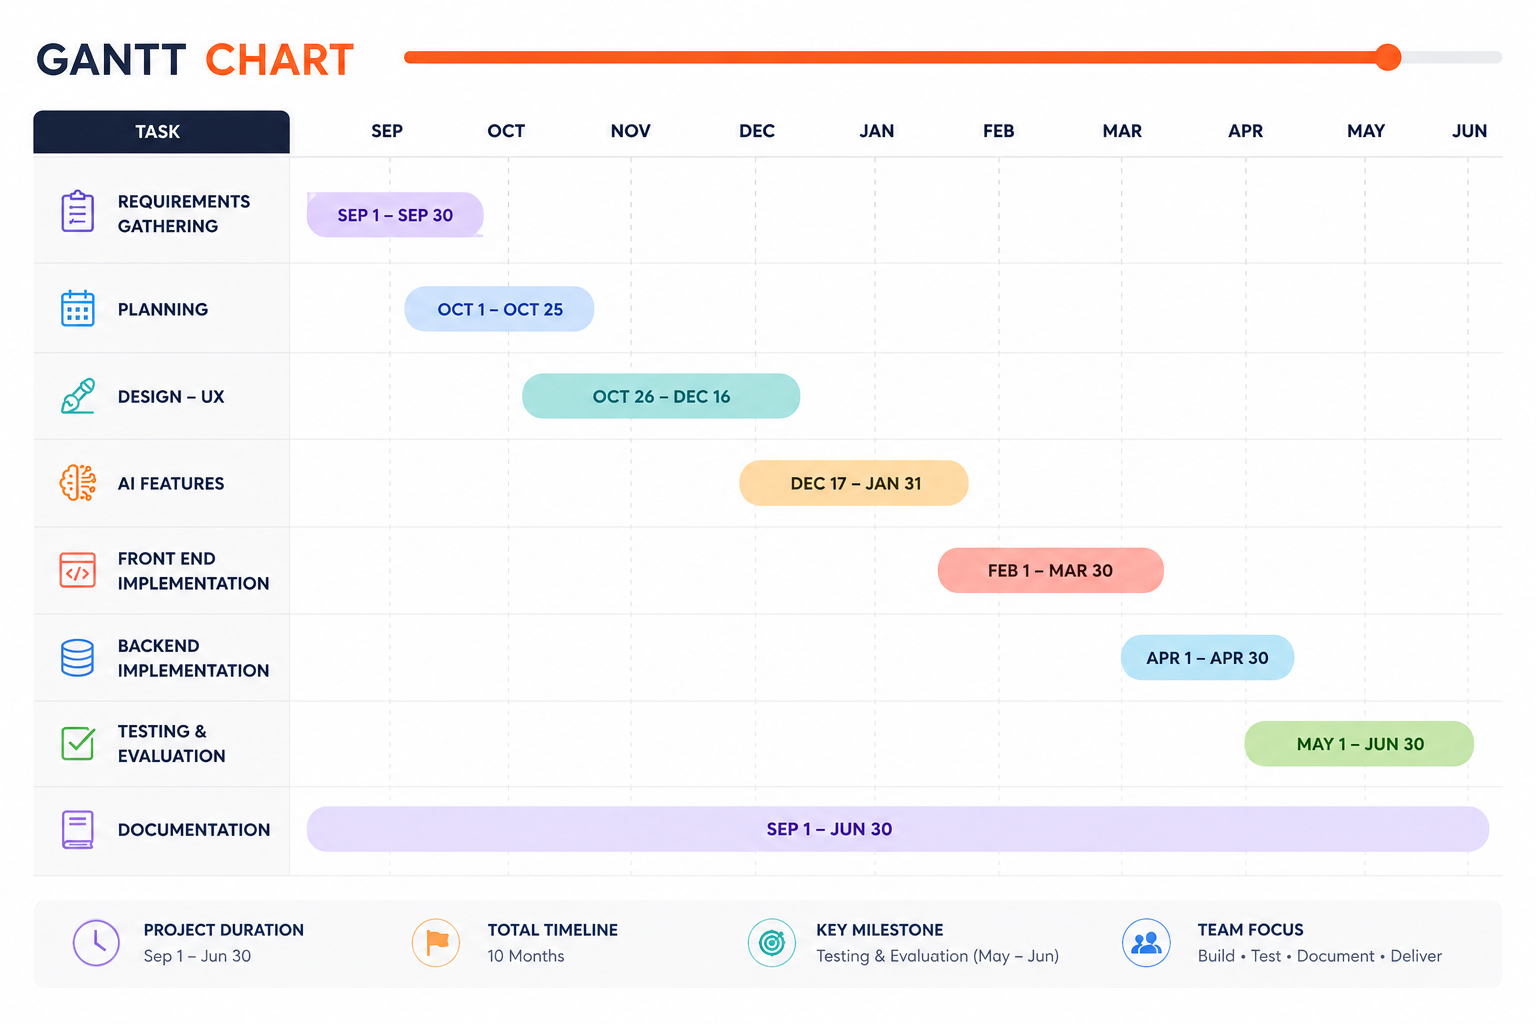
\includegraphics[width=0.95\linewidth,height=0.72\textheight,keepaspectratio]{images/img_033.png}
\caption{Project Timeline Gantt Chart}
\label{fig:chapter7-project-timeline}
\end{figure}

The timeline supported iterative development. When a module produced unexpected results, adjustments were made before moving to the next integration stage.

\section{Team Roles and Contributions}

VisionSafe360 required different development responsibilities, including AI development, backend development, frontend development, testing, and documentation. The work was organized by functional role so that each part of the project had clear ownership.

Table~\ref{tab:chapter7-team-roles} summarizes the main project roles and contribution areas.

\begin{table}[H]
\centering
\renewcommand{\arraystretch}{1.55}
\begin{tabular}{|>{\centering\arraybackslash}p{0.3\linewidth}|>{\centering\arraybackslash}p{0.58\linewidth}|}
\hline
\textbf{Role} & \textbf{Contribution Area} \\
\hline
\textbf{AI Model Development} & Dataset preparation, YOLO model training, pose analysis, fall rules, and hazard detection logic \\
\hline
\textbf{Backend Development} & API design, incident logging, alert management, WebSocket updates, and data handling \\
\hline
\textbf{Frontend Development} & Dashboard pages, live monitoring interface, alert views, reports, and ergonomic analytics interface \\
\hline
\textbf{Testing and Evaluation} & Test case design, model evaluation, runtime measurement, and result analysis \\
\hline
\textbf{Documentation} & Report writing, diagrams, tables, formatting, and final project organization \\
\hline
\end{tabular}
\caption{\textbf{Project roles and contribution areas}}
\label{tab:chapter7-team-roles}
\end{table}

This role-based organization helped the team work in parallel while keeping the system consistent. Integration meetings were used to combine the modules and resolve conflicts between the AI pipeline, backend services, and dashboard requirements.

\section{Risk Management}

Several risks were considered during project development. These risks included technical, operational, and documentation-related issues. Table~\ref{tab:chapter7-risk-management} presents the main risks and mitigation actions.

\begin{table}[H]
\centering
\renewcommand{\arraystretch}{1.55}
\begin{tabular}{|>{\centering\arraybackslash}p{0.28\linewidth}|>{\centering\arraybackslash}p{0.28\linewidth}|>{\centering\arraybackslash}p{0.32\linewidth}|}
\hline
\textbf{Risk} & \textbf{Impact} & \textbf{Mitigation} \\
\hline
\textbf{Low detection accuracy} & Incorrect or missed safety alerts & Improve dataset quality, tune thresholds, and apply persistence logic \\
\hline
\textbf{High false positives} & Alert fatigue for supervisors & Use confidence thresholds, cooldown periods, and temporal validation \\
\hline
\textbf{Low runtime performance} & Delayed real-time monitoring & Use GPU acceleration, optimized models, and controlled input resolution \\
\hline
\textbf{Camera perspective issues} & Inaccurate proximity estimation & Tune danger-zone thresholds and apply site-specific calibration \\
\hline
\textbf{Integration errors} & Broken communication between modules & Test APIs, backend events, and dashboard updates incrementally \\
\hline
\textbf{Privacy concerns} & Ethical and legal risk & Avoid raw video storage and apply anonymization principles \\
\hline
\end{tabular}
\caption{\textbf{Project risks and mitigation actions}}
\label{tab:chapter7-risk-management}
\end{table}

Risk management was important because VisionSafe360 is a safety-related system. The system must avoid both missed hazards and excessive false alarms, since both can reduce trust in the platform.

\section{Ethical and Legal Considerations}

VisionSafe360 processes workplace video streams, which makes ethics and privacy important parts of the project. The system is designed to support worker safety, not to monitor workers for punishment or unnecessary surveillance.

The main ethical principle is that the system should be used as a safety assistant for hazard prevention and faster response. Alerts should help HSE engineers and supervisors reduce risk, improve compliance, and prevent injuries. The system should not be used to unfairly evaluate workers without clear policies and proper communication.

Privacy was considered throughout the design. The project follows the principle of minimizing stored personal data. Raw video storage is avoided, and only safety-related metadata, alerts, and selected evidence snapshots should be stored when required. In a real deployment, face blurring or anonymization should be applied before saving or transmitting any visual evidence.

Legal considerations include compliance with workplace safety regulations, data protection requirements, and organizational camera-use policies. Workers should be informed that AI-assisted monitoring is used for safety purposes. Access to incident records should be restricted based on user roles, and sensitive evidence should be protected using secure authentication and encrypted communication.

Table~\ref{tab:chapter7-ethics} summarizes the main ethical and legal controls considered in the project.

\begin{table}[H]
\centering
\renewcommand{\arraystretch}{1.55}
\begin{tabular}{|>{\centering\arraybackslash}p{0.32\linewidth}|>{\centering\arraybackslash}p{0.56\linewidth}|}
\hline
\textbf{Area} & \textbf{Control} \\
\hline
\textbf{Privacy} & Avoid continuous raw video storage and keep only necessary safety records \\
\hline
\textbf{Anonymization} & Apply face blurring or identity protection before storing visual evidence \\
\hline
\textbf{Transparency} & Inform workers that the system is used for safety monitoring and incident prevention \\
\hline
\textbf{Access Control} & Limit dashboard and incident access based on user roles \\
\hline
\textbf{Data Security} & Use secure communication and protected storage for sensitive records \\
\hline
\textbf{Fair Use} & Use alerts for corrective safety actions rather than unfair worker punishment \\
\hline
\end{tabular}
\caption{\textbf{Ethical and legal controls}}
\label{tab:chapter7-ethics}
\end{table}

These controls help ensure that the system improves workplace safety while respecting privacy, fairness, and responsible AI use.

\section{Sustainability and Societal Impact}

VisionSafe360 contributes to sustainability by improving occupational safety and reducing preventable workplace injuries. Safer workplaces reduce downtime, medical costs, equipment damage, and operational disruption. The system also supports preventive safety practices by identifying risks before they become serious incidents.

The ergonomic analysis module has a long-term societal benefit because musculoskeletal injuries often develop slowly and may not be reported immediately. By monitoring posture trends, HSE teams can identify risky tasks, redesign workflows, and reduce long-term worker health problems.

From an environmental and economic perspective, the system is designed to work with existing CCTV infrastructure. This reduces the need for specialized hardware and allows organizations to reuse cameras already installed in industrial sites. Edge processing also reduces the amount of video data sent over networks, lowering bandwidth usage and improving privacy.

Table~\ref{tab:chapter7-sustainability} summarizes the sustainability and societal impact of the project.

\begin{table}[H]
\centering
\renewcommand{\arraystretch}{1.55}
\begin{tabular}{|>{\centering\arraybackslash}p{0.32\linewidth}|>{\centering\arraybackslash}p{0.56\linewidth}|}
\hline
\textbf{Impact Area} & \textbf{Contribution} \\
\hline
\textbf{Worker Safety} & Faster detection of PPE violations, falls, and unsafe proximity events \\
\hline
\textbf{Health Protection} & Early identification of ergonomic posture risks and harmful repeated movements \\
\hline
\textbf{Economic Benefit} & Reduced accident costs, downtime, and manual reporting effort \\
\hline
\textbf{Environmental Benefit} & Reuse of existing camera infrastructure and reduced need for additional sensors \\
\hline
\textbf{Operational Sustainability} & Scalable modular design that can be expanded to more cameras and sites \\
\hline
\textbf{Social Responsibility} & Supports a safer working culture and proactive hazard prevention \\
\hline
\end{tabular}
\caption{\textbf{Sustainability and societal impact}}
\label{tab:chapter7-sustainability}
\end{table}

Overall, VisionSafe360 supports safer industrial operations and encourages a shift from reactive incident handling to proactive risk prevention.

\section{Chapter Summary}

This chapter discussed project management, team organization, risks, ethical considerations, and sustainability aspects of VisionSafe360. The work breakdown structure and timeline showed how the project was organized from requirements analysis to final testing and documentation.

The chapter also highlighted the importance of privacy, transparency, access control, and fair use because the system works with workplace video data. Finally, the sustainability discussion showed how VisionSafe360 can support worker safety, reduce long-term health risks, and improve safety culture through AI-assisted monitoring.


% ---------------------------------------------------------
% BIBLIOGRAPHY (optional - included only if references.bib exists)
% ---------------------------------------------------------
\IfFileExists{references.bib}{%
	\bibliographystyle{ieeetr}
	\bibliography{references}
}{}

\end{document}
